\documentclass[a4paper, 12pt]{scrartcl}
\usepackage{scrpage2}
\usepackage[left=2.5cm,right=2.5cm, top=3cm, bottom=4cm]{geometry}
\usepackage[utf8]{inputenc}
\usepackage[ngerman]{babel}
\usepackage[T1]{fontenc}
\usepackage{amsmath}
\usepackage{amssymb}
\usepackage{amsfonts}

\usepackage{graphicx}
\usepackage{subfigure}

\usepackage{float}
\usepackage{adjustbox}
\usepackage{hyperref}
\usepackage{textcomp}
\usepackage{multirow}
\usepackage{array}

%\usepackage{enumerate}
\usepackage[shortlabels]{enumitem}

%Zeichnungen
\usepackage{tikz}
\usepackage[european]{circuitikz}

% Einrücken verhindern
\setlength{\parindent}{0em} 


\begin{document}

\begin{titlepage}
	\centering
	{\Huge\bfseries Versuchsprotokoll\par}
	\vspace{2cm}
	{\scshape\LARGE Elektrizitätslehre \par}
	\vspace{1cm}
	{\Large Gedämpfter LCR-Schwingkreis und \\ Gekoppelte LC-Schwingkreise\par}
	\vfill
	{\large\itshape Simon Schwarz und Marius Ising\par}

	\vfill
\end{titlepage}

\tableofcontents
\newpage


\section{Gedämpfter LCR-Schwingkreis}


\subsection{Versuchsbeschreibung}

In einer Serienschaltung aus Spule $L$, Kondensator $C$ und Ohmschem Widerstand $R$ (vgl. Abb. \ref{abb:schaltLCR}) wird der Kondensator zunächst aufgeladen und anschließend die Spannungsquelle mit einem Taster überbrückt, sodass der Kondensator sich über den Widerstand entladen kann. Dabei entlädt sich der Kondensator nicht sofort, sondern er schwingt sich bei der Spannung $U=0$ ein. Dieser Einschwingvorgang hängt wesentlich von der Dämpfung der Schwingung durch die Ohmschen Widerstände der Schaltung ab.

\begin{figure}[H]
\centering
\begin{tikzpicture}
\draw (2,0) node[ocirc]{} -- (2,1) to [C, a=$C$] (2,3) to [R, a=$R$] (4,3)  to [cute inductor, a=$L$] (6,3) to[rmeterwa, t=$I$] (6,1) -- (6,0) node[ocirc]{};
\draw (2,1) to [push button] (6,1);
\draw (2,1.2) -- (1,1.2) to [rmeterwa, t=$U_C$] (1,2.8) -- (2,2.8);
\end{tikzpicture}
\caption{Schaltbild des LCR-Schwingkreises}
\label{abb:schaltLCR}
\end{figure}

Nach der Kirchhoffschen Maschenregel gilt für die Schaltung bei gedrücktem Taster
$$0 = U_C + U_R + U_L = \frac QC + RI + L \frac{dI}{dt}$$
Mit $I = \frac{dQ}{dt}$ erhält man folgende Differentialgleichung
$$\frac{d^2Q}{dt^2} + \frac{R}{L} \frac{dQ}{dt} + \frac{1}{LC}Q = 0$$
Dies ist die DGL einer gedämpften harmonischen Schwingung. Dabei bezeichnet $\delta = \frac{R}{2L}$ die Dämpfungskonstante und $\omega_0 = \frac{1}{\sqrt{LC}}$ die Schwingungsfrequenz der ungedämpften Schwingung. 
Für die Lösung der DGL unterscheiden wir drei Fälle. In allen Fällen gelten die gleichen Anfangsbedingungen
$$Q(0) = CU_0 \hspace{0.5cm} \text{ und } \hspace{0.5cm} I(0) = 0.$$

\textbf{Schwingfall ($\delta < \omega_0$)} \\
Hier ist eine echte Schwingung zu beobachten. Es gilt
$$Q(t) = e^{-\delta t}( A\cos(\omega t) + B\sin(\omega t)).$$
Aus den Anfangsbedingungen erhält man $A = CU_0$ und $B = A \frac{\delta}{\omega}$. Für den Strom gilt wegen $I = \frac{dQ}{dt}$
\begin{equation}\label{eq:i_lsg}
I(t) = -CU_0 e^{-\delta t} \left( \omega + \frac{\delta^2}{\omega}\right)\sin(\omega t)\text{.}
\end{equation}

\textbf{Kriechfall ($\delta > \omega_0$)} \\ 
In diesem Fall ist die Dämpfung so stark, dass der Kondensator seine Spannung nur sehr langsam verliert. Zudem findet keine Schwingung statt.
$$Q(t) = Ae^{\left( -\delta + \sqrt{\delta^2-\omega_0^2} \right)t} + Be^{\left(-\delta - \sqrt{\delta^2-\omega_0^2} \right)t}$$
Aus den Anfangsbedingungen ergibt sich
$$A = CU_0 \frac{\delta +\sqrt{\delta^2-\omega_0^2}}{2\sqrt{\delta^2-\omega_0^2}} \hspace{0.5cm} \text{ und } \hspace{0.5cm}
B = CU_0 \frac{-\delta+\sqrt{\delta^2-\omega_0^2}}{2\sqrt{\delta^2-\omega_0^2}}$$

\textbf{Aperiodischer Grenzfall ($\delta = \omega_0$)} \\
Der Kondensator wird innerhalb der kürzesten Zeit entladen. Die Lösung hat die Form
$$Q(t) = e^{-\delta t}(A + Bt)$$
mit $A = CU_0$ und $B=\delta A$.


\subsection{Versuchsaufbau}

\begin{figure}[H]
\centering
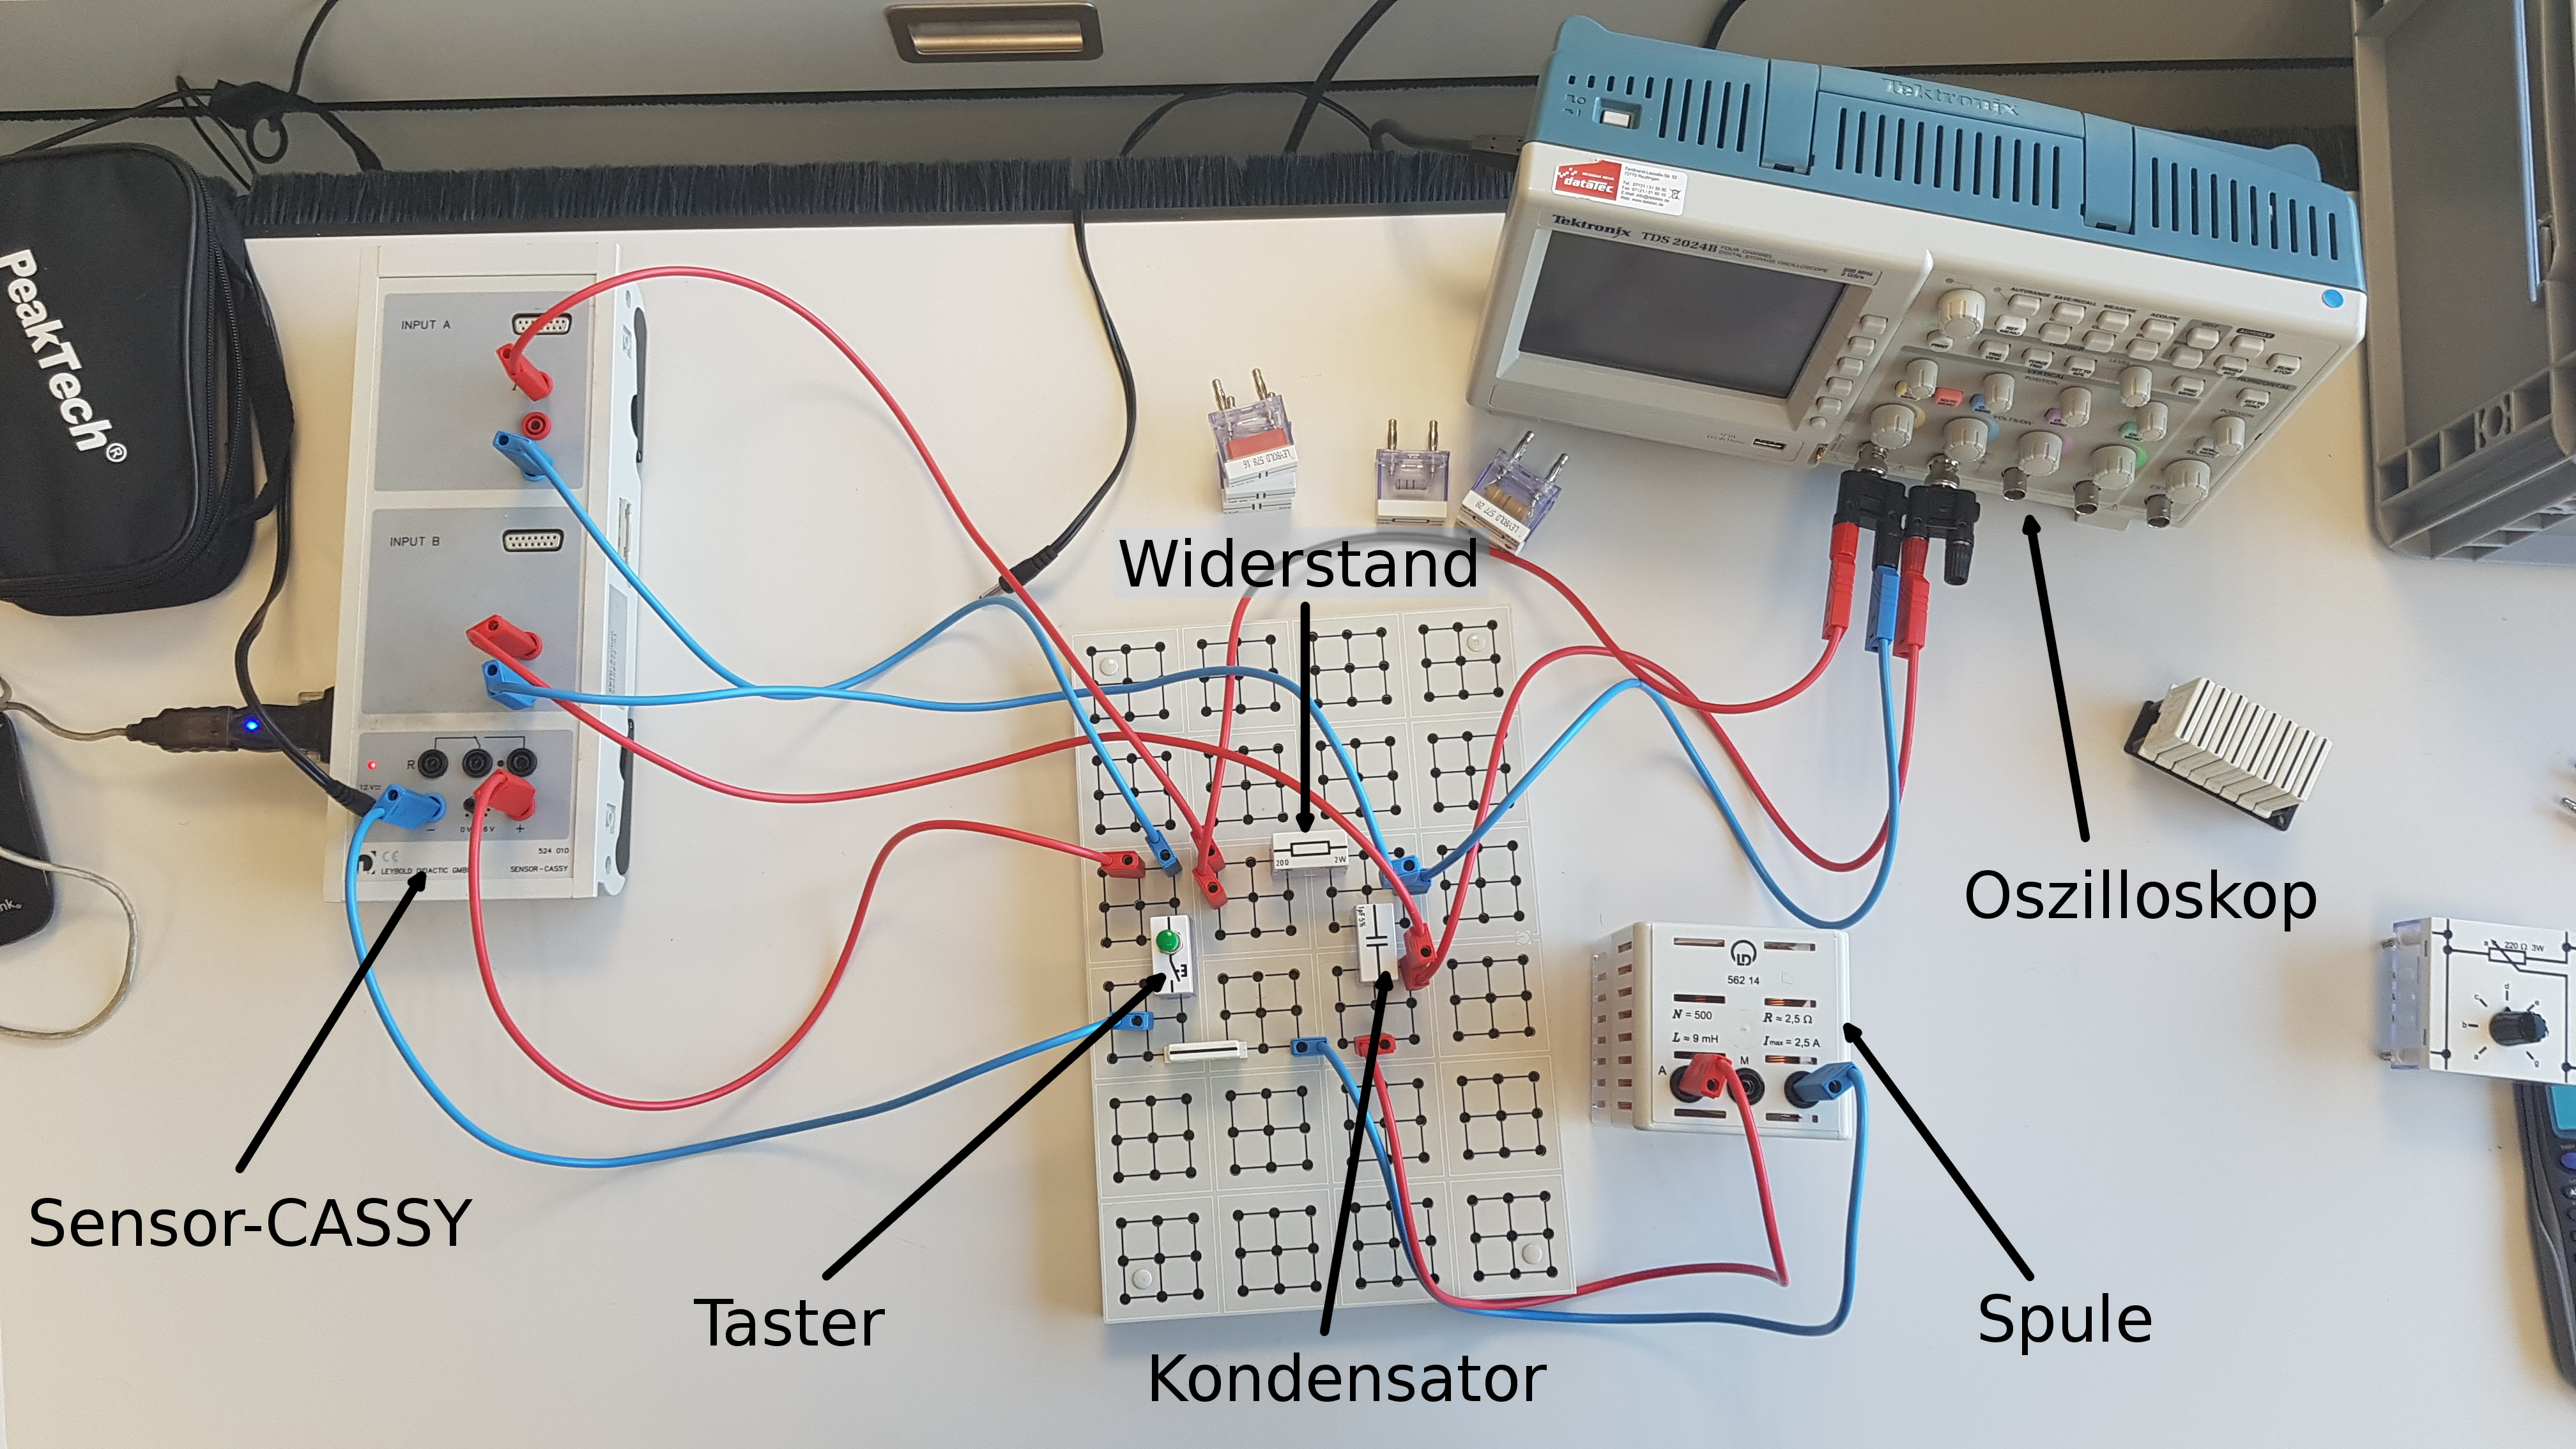
\includegraphics[width=\textwidth]{bilder/LCR_aufbau_beschriftet.jpg}
\caption{Versuchsaufbau LCR-Schwingkreis}
\label{abb:aufbau_lcr}
\end{figure}
Das Schaltbild aus Abbildung \ref{abb:schaltLCR} wird auf der Rastersteckplatte aufgebaut. Dies ist in Abbildung \ref{abb:aufbau_lcr} zu sehen. Als Spannungsquelle dient die Spannungsquelle des Sensor-CASSY. Die Spannung am Kondensator wird am Eingang B und die Stromstärke am Eingang A gemessen. Zusätzlich wird die Spannung am Kondensator am Channel 1 und die Spannung am Widerstand am Channel 2 des Oszilloskops gemessen. Die Erde liegt dabei zwischen Kondensator und Widerstand.

\subsection{Versuchsdurchführung}

Die Schwingungen werden im Modus \glqq automatische Aufnahme\grqq{} mit folgenden Messparametern aufgenommen:
\begin{enumerate}[-]
\setlength{\itemsep}{-5pt}
\item Messbereich Strom $I$: $\pm 0.3$ A
\item Messbereich Spannung am Kondensator $U_C$: $\pm 10$ V
\item Messintervall: $10 \, \mu\text{s}$
\item Anzahl an Messpunkten: $2000$
\item Messzeit: $20$ ms
\end{enumerate}
Die Spannungsquelle des Sensor-CASSYs ist stets eingeschaltet, so dass der Kondensator geladen ist. Eine Messung wird ausgelöst, indem der Taster gedrückt und somit der Stromkreis geschlossen wird. Um möglich direkt nach Betätigung des Tasters die Aufnahme zu beginnen, wird ein Trigger verwendet. Dieser aktiviert die Messung bei einer steigenden Flanke von $U_C$, die den Schwellenwert von $-9.2 \, \mathrm V$ überschreitet. Das ist sinnvoll, weil die Spannungsquelle auf $U_0 = 9.4 \, \mathrm V$ eingestellt ist und die Polung des Messgerätes zu einer gemessenen Kondensatorspannung von $-9.4 \, \mathrm V$ bei offenem Taster führt. 
Vorab werden die im Versuch verwendeten Widerstände mit Hilfe eines Multimeters auf ihren tatsächlichen Widerstandswert geprüft. In Tabelle \ref{tab:widerstaende} sind die verwendeten Widerstände mit Herstellerangabe und gemessenen Werten angegeben.

\begin{table}[H]
\centering
\begin{tabular}{c|c}
Herstellerangabe / $\Omega$ & Gemessener Wert / $\Omega$ \\
\hline
$1$ & $1.008 \pm 0.001$ \\
$5.1$ & $5.101 \pm 0.001$ \\
$10$ & $9.990 \pm 0.002$ \\
$20$ & $19.82 \pm 0.01$ \\
$47$ & $46.67 \pm 0.01$ \\
$100$ & $99.24 \pm 0.04$ \\
$1000$ & $991.20\pm 0.08$
\end{tabular}
\caption{Herstellerangaben für die verwendeten Widerstände und deren mittels Multimeter gemessene Widerstandswerte samt Fehler.}
\label{tab:widerstaende}
\end{table}
Ebenso wurde die verwendete $9 \,$mH Spule und der $1 \, \mu$F Kondensator überprüft. Es ergab sich eine Induktivität von $(9.00 \pm 0.01)\,$mH und eine Kapazität von $(984.2 \pm 0.2)\,$nF.
Die nun folgenden Rechnungen verwenden die gemessenen Widerstandswerte. Zusätzlich werden drei in Reihe geschaltete $1\,\text{k}\Omega$ Widerstädnde verwendet, um einen Widerstand von $3\,\text{k}\Omega$ zu erreichen. Da diese Messung jedoch nur zur Visualisierung des Kriechsfalls dient, wird kein genauer Wert benötigt. Um den aperiodischen Grenzfall einzustellen, wird außerdem ein Potentiometer verwendet. Durch sukzessives Erhöhen des Widerstandes nimmt $\delta$ zu, sodass ab einem gewissen Wert keine Schwingung mehr am Oszilloskop beobachtbar ist. Dieses Vorgehen wird in Abbildung \ref{pic:oszi} dargestellt.

\begin{figure}[h]
\centering
\subfigure[$60\,\Omega$]{
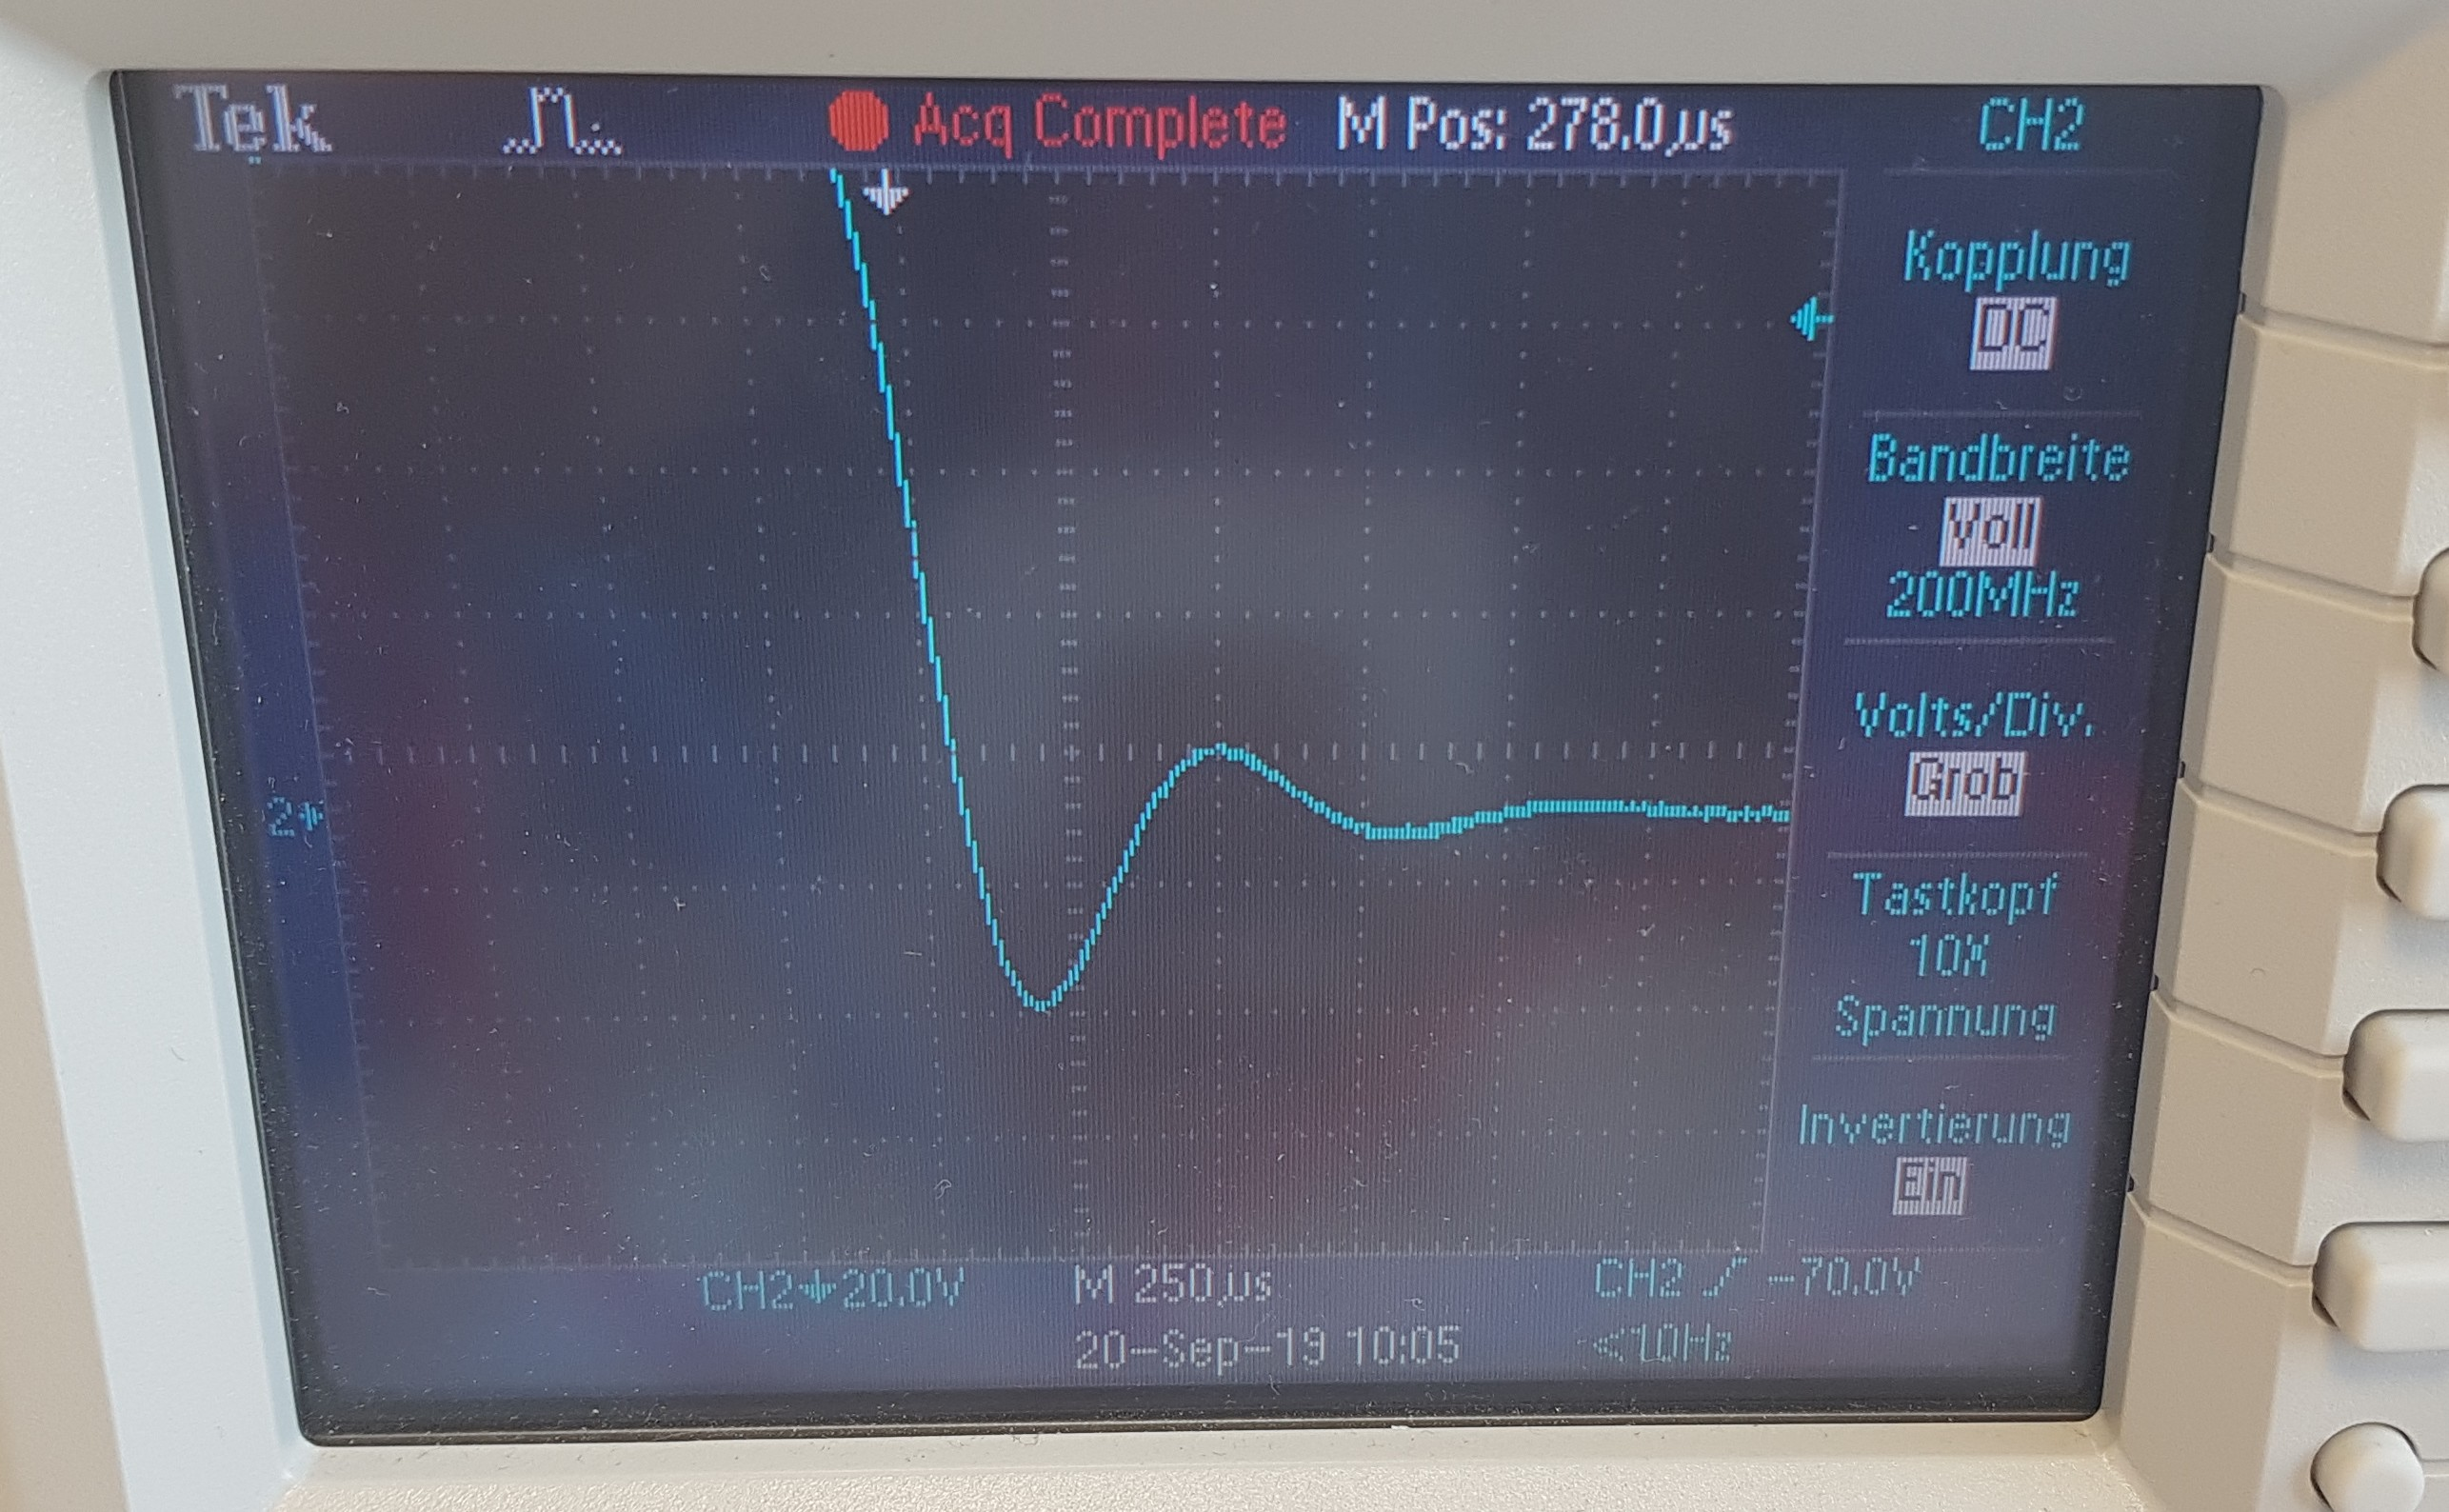
\includegraphics[width=.37\textwidth]{bilder/oszi1.jpg}
}
\subfigure[$160\,\Omega$]{
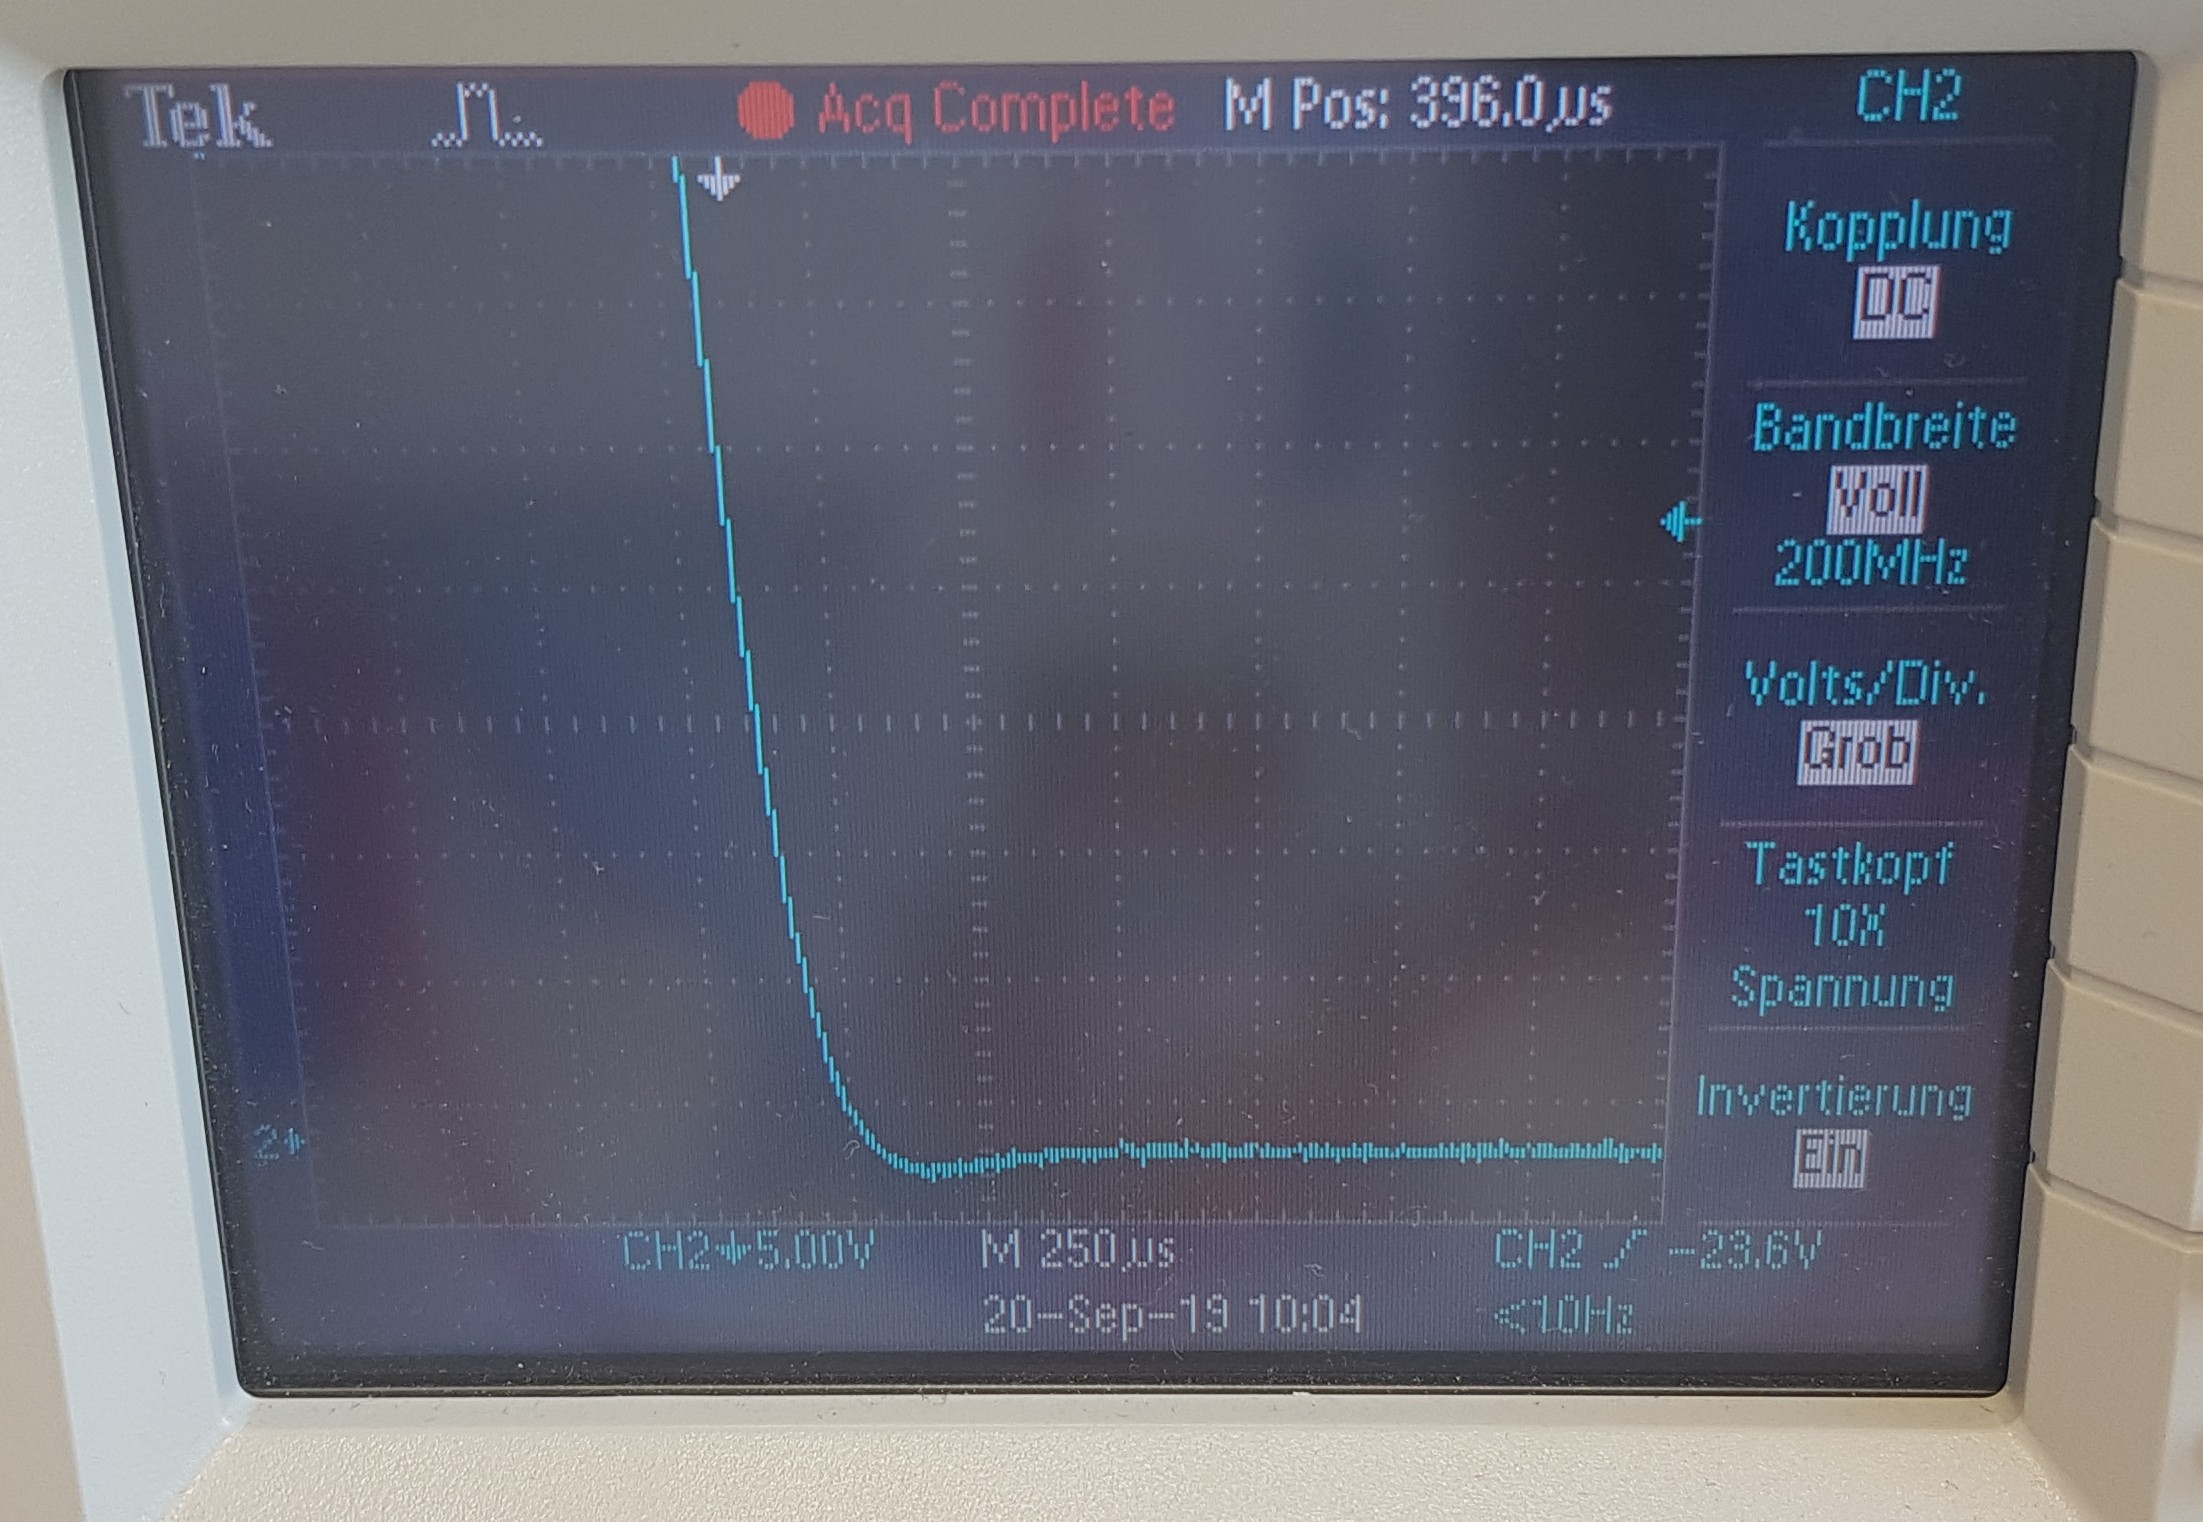
\includegraphics[width=.37\textwidth]{bilder/oszi2.jpg}
}

\subfigure[$186\,\Omega$]{
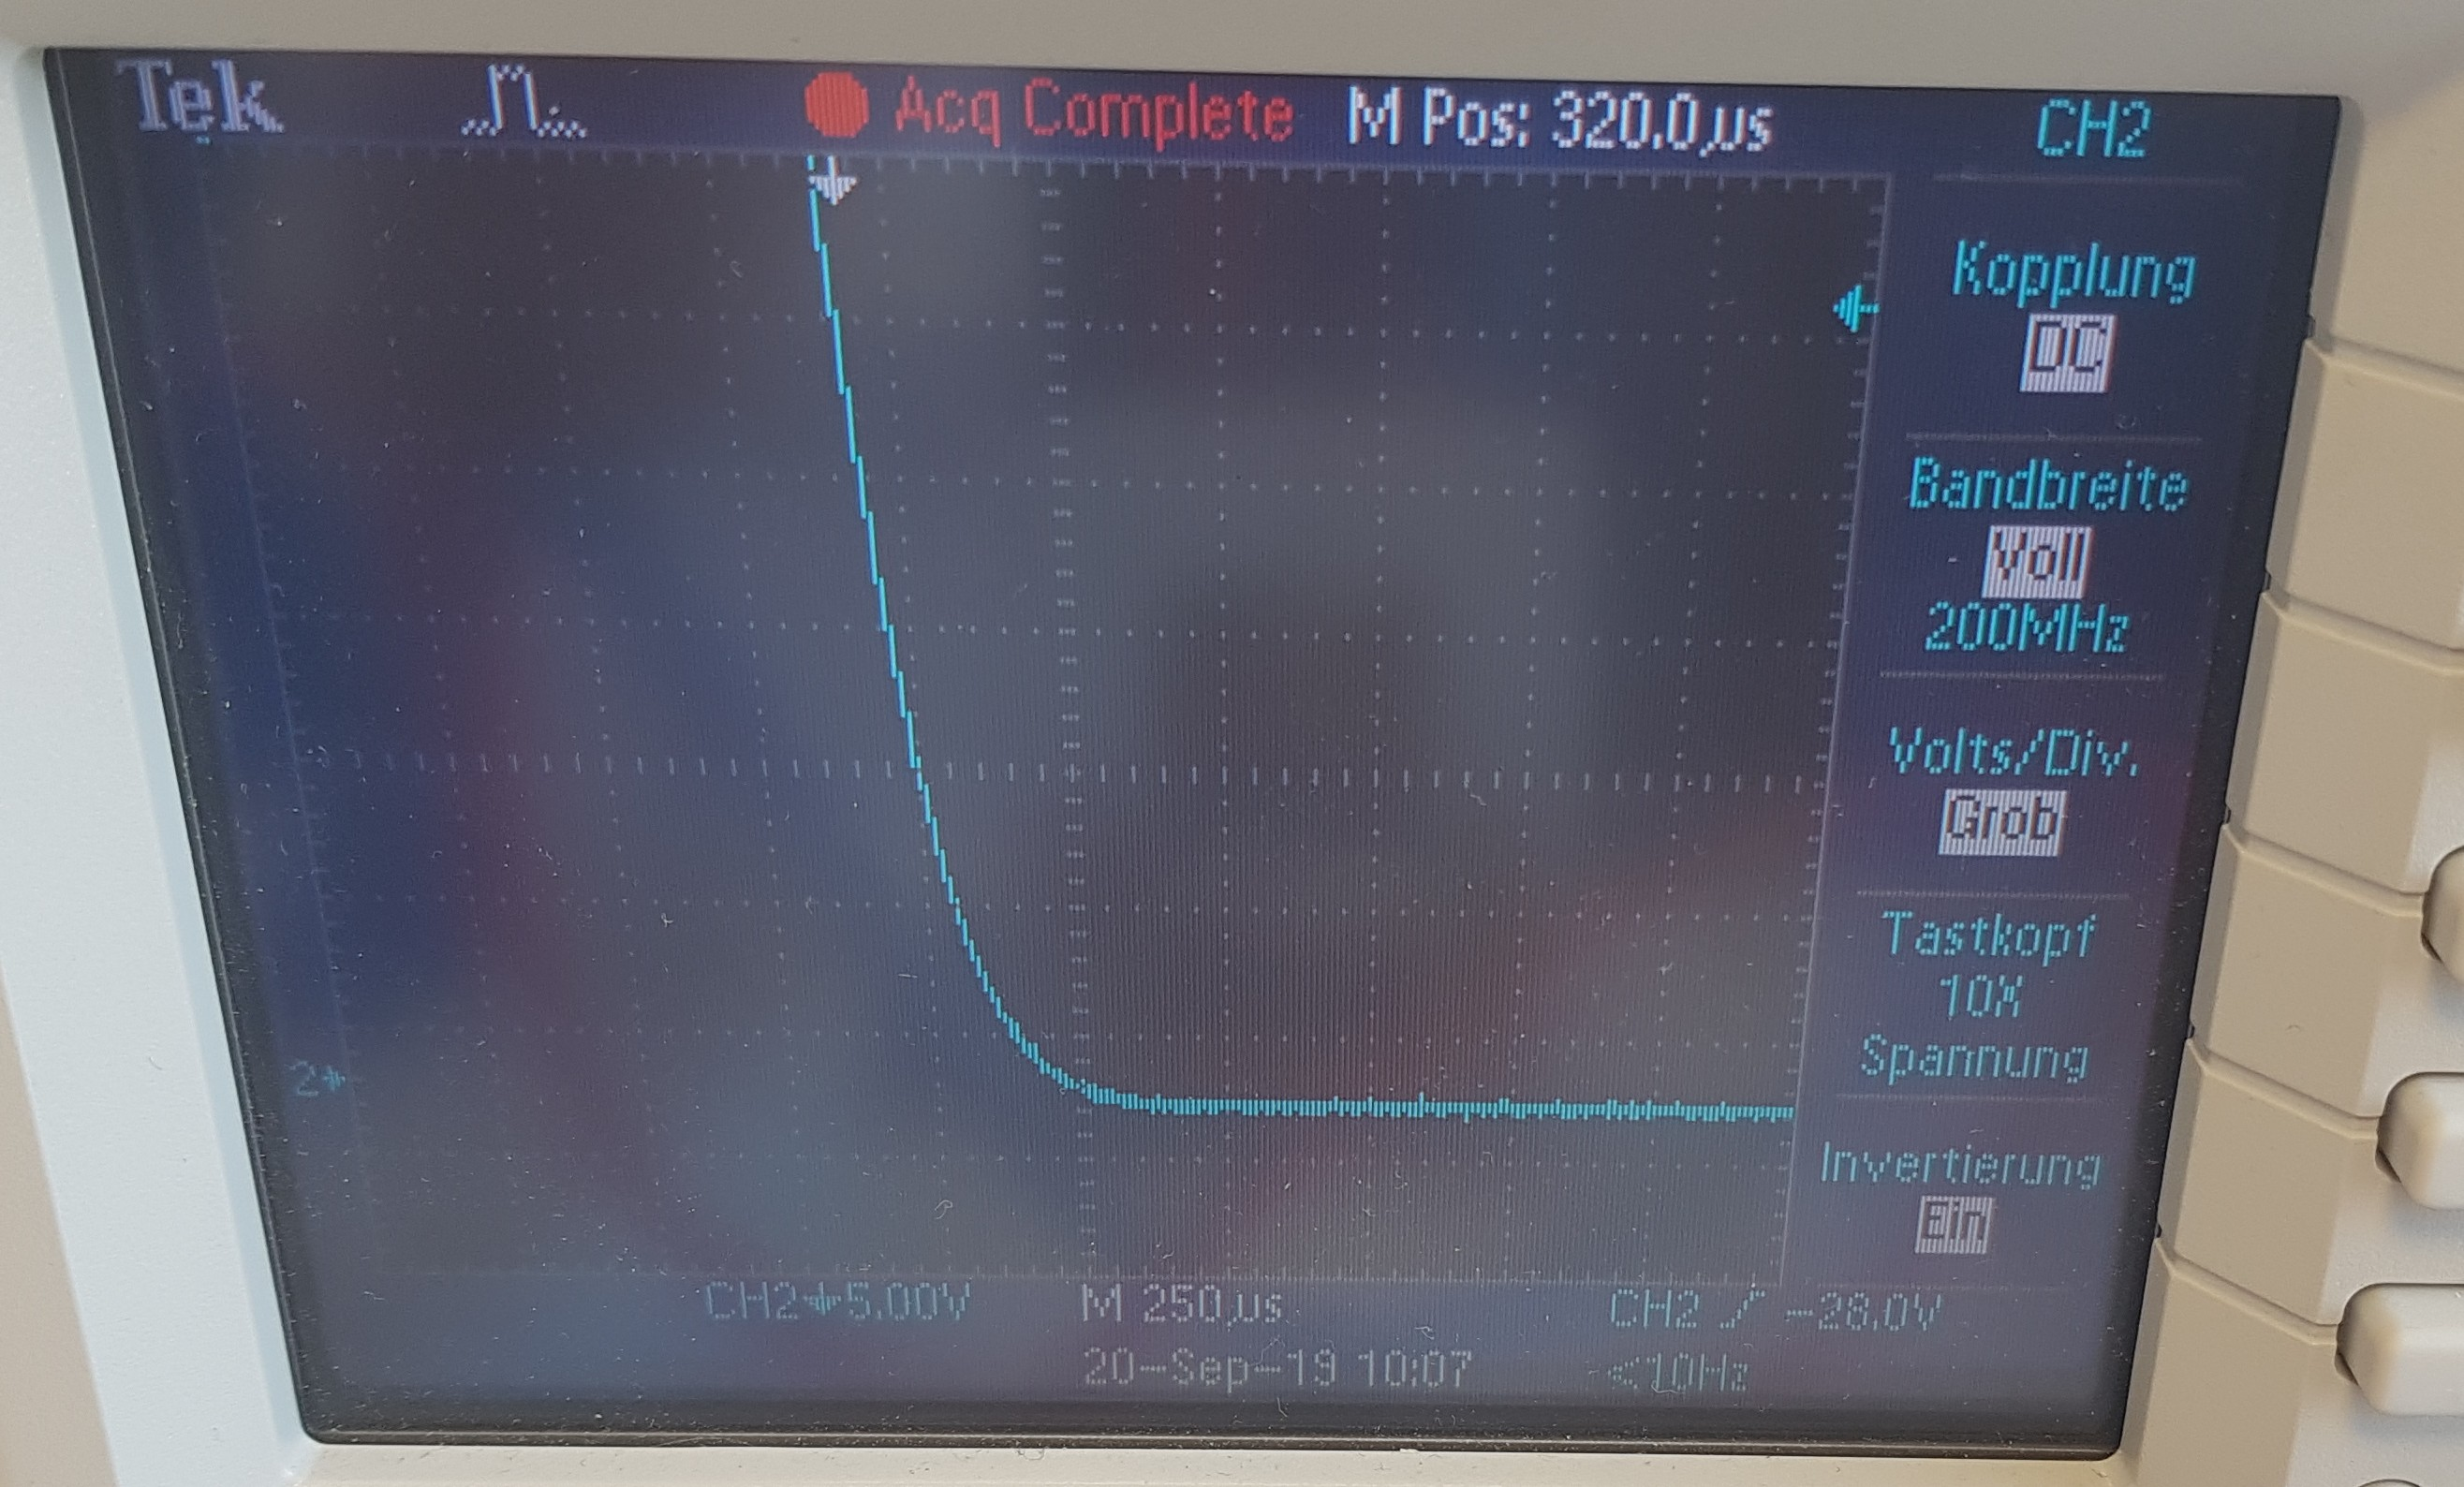
\includegraphics[width=.37\textwidth]{bilder/oszi3.jpg}
}
\caption{Messungen der Schwingung mit verschiedenen Einstellungen des Potentiometers. Man erkennt gut, wie durch das Erhöhen des Widerstandwertes die Schwingung abnimmt.}
\label{pic:oszi}
\end{figure}

\subsection{Versuchsauswertung}

Beispielhafte Rohdaten für alle verschiedenen Fälle sind in Abbildung \ref{abb:rohdaten_ska} zu sehen.

\begin{figure}[H]
\centering
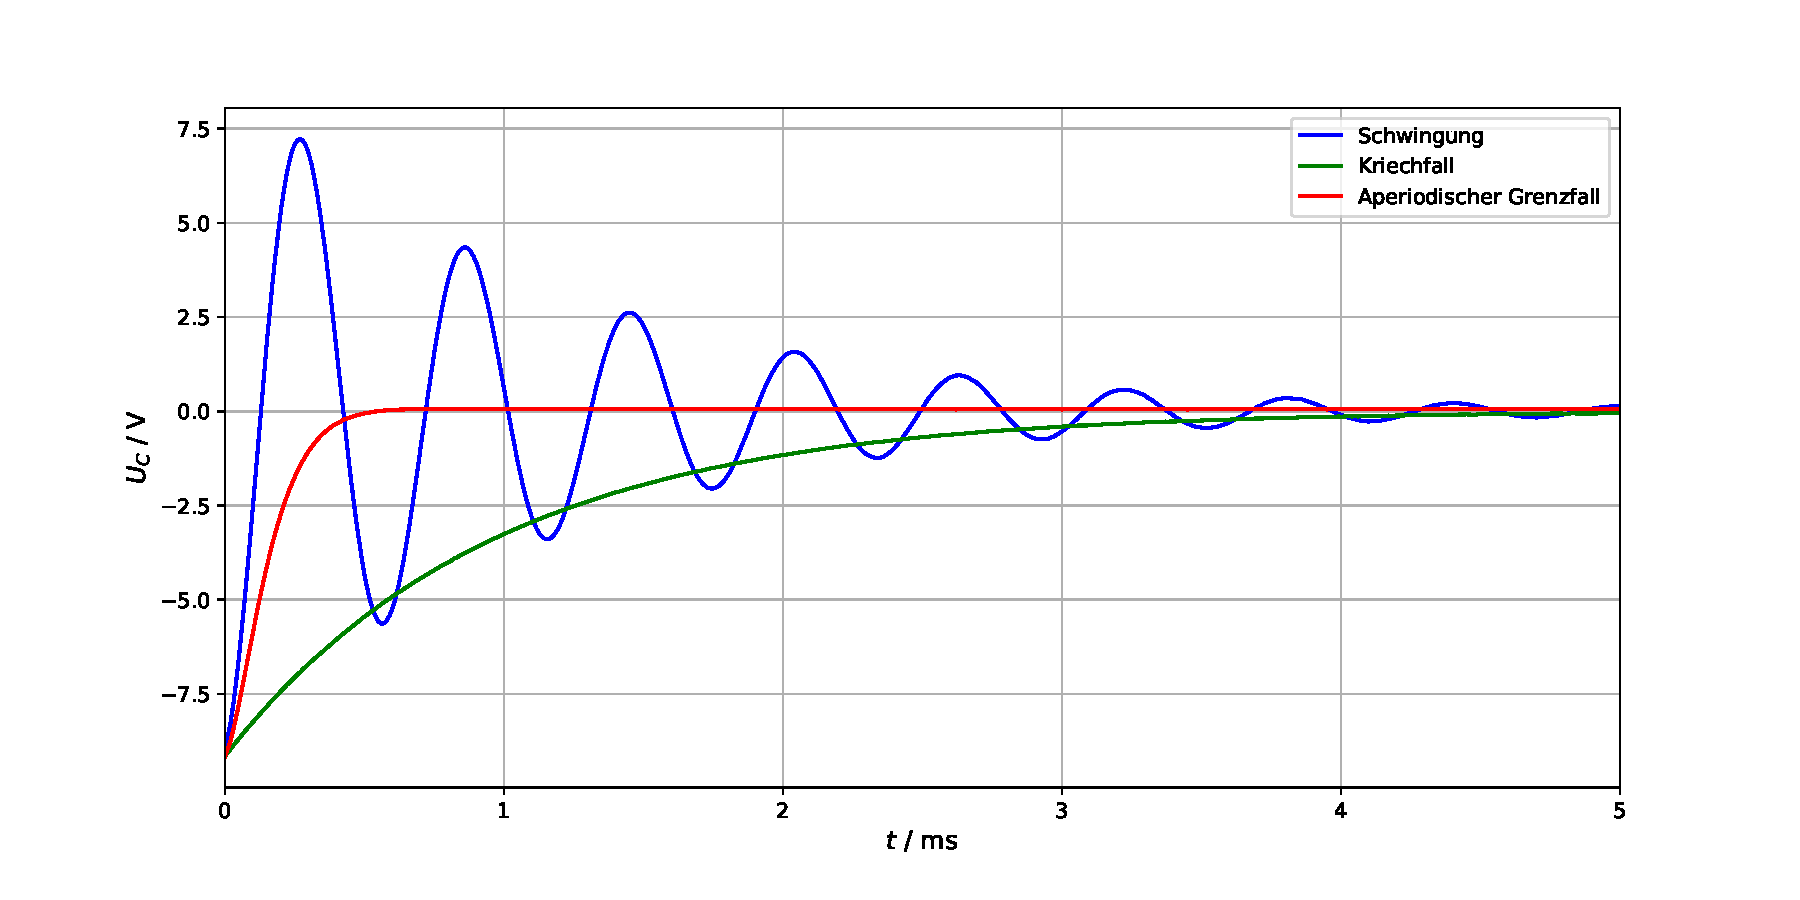
\includegraphics[width=.9\textwidth]{plots/rohdaten_ska.pdf}
\caption{Rohdaten mit Schwing-, Kriech- und Aperiodischem Grenzfall}
\label{abb:rohdaten_ska}
\end{figure}

\subsubsection{Schwingfall}
Zunächst bestimmen wir die Frequenzen und die Dämpfungen der aufgenommenen Schwingungen für die verschiedenen verwendeten Ohmschen Widerstände. Um die Frequenz bzw. die Periodendauer zu bestimmen, existieren zwei Möglichkeiten. Einerseits ist die Analyse mittels FFT möglich. Andererseits können die Extrema aus den Rohdaten abgelesen und die Periodendauer mittels Regression über die Schwingungsanzahl bestimmt werden.
Analog dazu besteht die Möglichkeit, die Dämpfung $\delta$ aus Gleichung \ref{eq:i_lsg} durch logarithmisches Auftragen der Extrema, d.h. mit Regression, zu berechnen: Es gilt
$$sin(\omega t_i) = \pm 1$$
für die Zeitpunkte $t_i$ an denen $I$ bzw. $U_C$ ein Extremum annimmt. Durch logarithmieren der Gleichung \ref{eq:i_lsg} erhält man für diese Zeiten $t_i$ dann
$$\log \lvert I(t_i)\rvert = -\delta t_i + \log\left\lvert CU_0 \left(\omega+\frac{\delta^2}{\omega}\right)\right\rvert$$
beziehungsweise eine analoge Form für $U_C$. Natürlich kann $\delta$ durch die Verwendung eines Steigungsdreiecks auch nur bei zwei ablesbaren Maxima oder Minima bestimmt werden:
$$\delta = \frac{\log\left(\frac{U_C(t_0)}{U_C(t_1)}\right)}{t_1-t_0}$$
Bei beiden Vorgehensweisen muss der Offset korrigiert werden. Als zweite Option für die Berechnung von $\delta$ kann eine Exponentialfunktion als Einhüllende gefittet werden und die Dämpfung $\delta$ aus dem Fit abgelesen werden.
Für den $100\,\Omega$ Widerstand sind Regressionen nicht praktikabel, da - aufgrund der starken Dämpfung - zu wenige Extrema genau ablesbar sind. Ein beispielhaftes Ergebnis für die Regression von abgelesenen Extrema bei der Schwingung des $10\,\Omega$ Widerstand ist in Abbildung \ref{abb:reg1} dargestellt. Die übrigen durchgeführten Regressionen sind im Anhang \ref{app:reg} abgebildet.

\begin{figure}[h]
\centering
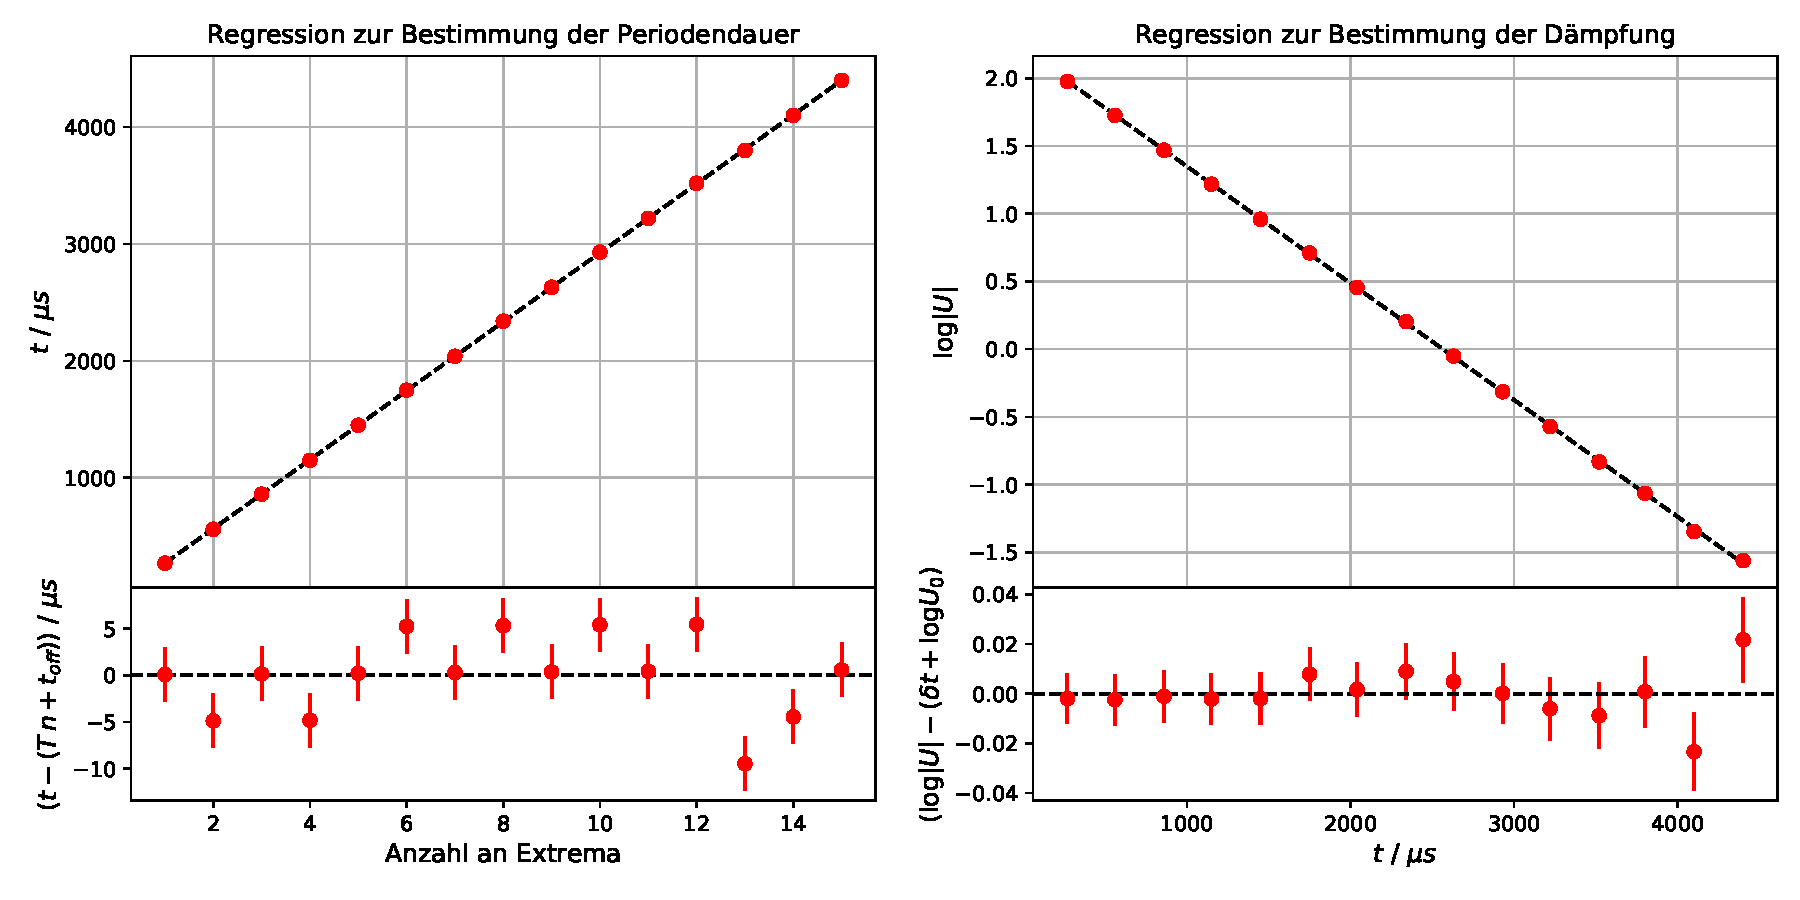
\includegraphics[width=\textwidth]{plots/reg_schwingung3.pdf}
\caption{Regressionen für den $10\,\Omega$ Widerstand zur Bestimmung von $\frac{T}{2}$ und $\delta$.}
\label{abb:reg1}
\end{figure}

\begin{figure}[h]
\centering
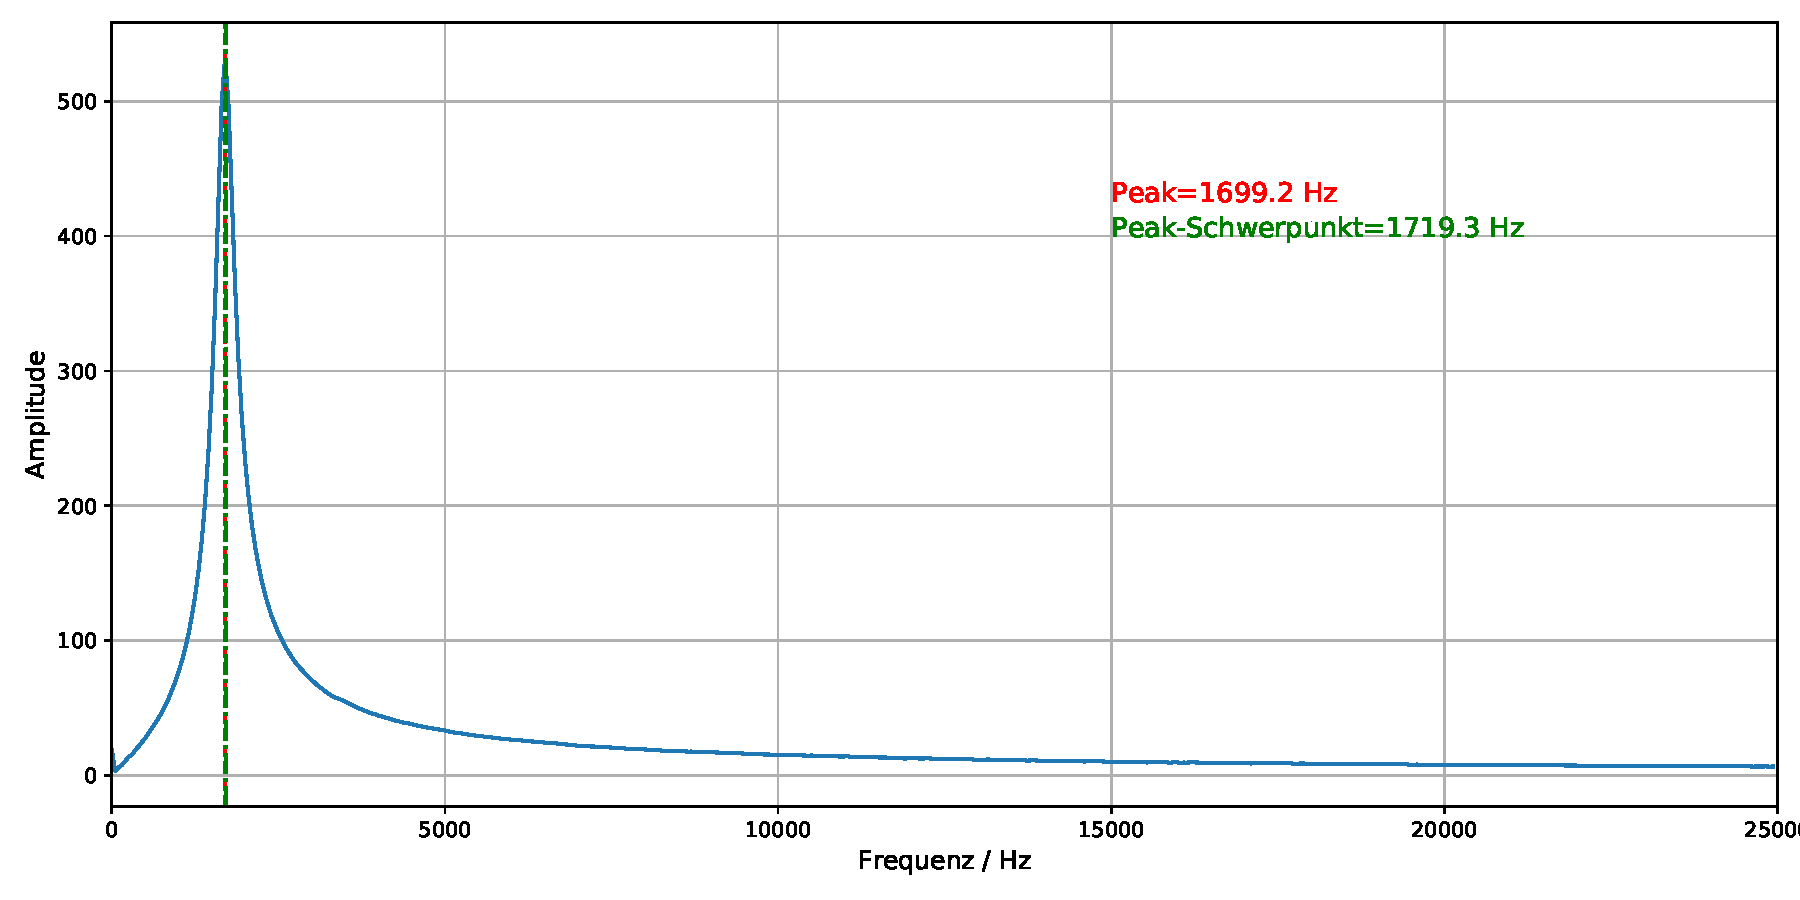
\includegraphics[width=\textwidth]{plots/fft/fft_schwingung3_1.pdf}
\caption{Mittels FFT berechnetes Spektrum für die erste Messung des $10\,\Omega$ Widerstands. Die rote Linie zeigt das Argument-Maximum an. Die grüne Linie Hingegen den Peak-Schwerpunkt.}
\label{abb:fft1}
\end{figure}

Für die Frequenzen ergeben sich die in Tabelle \ref{tab:freq} dargestellten Werte. Die FFT-Ergebnisse sind mit der Peakfinder-Methode berechnet. Dabei sollte man beachten, dass der FFT-Algorithmus die Frequenz mit einer Breite von $h\approx 49.975 \,\text{Hz}$ diskretisiert. Dies mindert die Qualität der Resultate spürbar. Als Fehler der Einzelmessungen wird die Differenz aus Argument-Maximum der Amplitude und Peak-Schwerpunkt verwendet. Der Fehler des gewichteten Mittels ist der innere Fehler der Einzelmessungen. Das Frequenzspektrum der ersten Messung des $10\,\Omega$ Widerstands ist in Abbildung \ref{abb:fft1} zu sehen. Für die übrigen Widerstände befindet sich jeweils das Spektrum der 1. Messung im Anhang \ref{app:fft}.

\begin{table}[H]
\centering
\begin{adjustbox}{width=\textwidth}
\begin{tabular}{c|c|cccc}
\multirow{2}{*}{Widerstand / $\Omega$} & \multirow{2}{*}{Regression / Hz} & \multicolumn{4}{c}{$f$ mit FFT / Hz} \\
\cline{3-6}
& & Messung 1 & Messung 2 & Messung 3 & Mittel\\
\hline
$1$ & $1696.9 \pm 0.6$ & $1715.7\pm 16.6$ & $1715.2\pm 16.1$ & $1715.3\pm 16.1$ & $1715.4\pm 9.4$\\
$5.1$ & $1696.3 \pm 0.7$ & $1718.9\pm 19.7$ & $1719.0\pm 19.8$ & $1719.0\pm 19.8$ & $1718.9\pm 11.4$\\
$10$ & $1695.1 \pm 1.0$ & $1719.3\pm 20.1$ & $1719.3\pm 20.1$ & $1719.2\pm 20.0$ & $1719.2\pm 11.6$ \\
$20$ & $1689.2 \pm 2.1$ & $1720.4\pm 21.3$ & $1720.3\pm 21.2$ & $1720.3\pm 21.2$ & $1720.4\pm 12.2$\\
$47$ & $1628.6 \pm 4.8$ & $1761.1\pm 62.0$ & $1761.3\pm 62.1$ & $1741.5\pm 42.4$ & $1751.0 \pm 30.5$\\
$100$ & - & $1294.7\pm 154.6$ & $1293.4\pm 155.8$ & $1339.0\pm 110.3$ & $1316.4 \pm 77.8$
\end{tabular}
\end{adjustbox}
\caption{Mit Regression und FFT ermittelte Frequenzwerte.}
\label{tab:freq}
\end{table}

Die Messungen des $100\,\Omega$ Widerstands werden von nun an nicht weiter ausgewertet, da die kurze Schwingzeit keine zuverlässigen Ergebnisse ermöglicht. Des Weiteren arbeitet die Peakfinder-Methode wegen der groben Diskretisierung der Frequenz durch den FFT-Algorithmus nicht korrekt, sodass die Frequenzen der Regressionsmethode als weitere Berechnungsgrundlage dienen. Ein Indiz dafür, dass die Frequenzwerte aus dem Spektrum systematisch fehlerhaft sind, ist, dass sie mit steigendem Widerstand steigen, obwohl
\begin{equation}\label{eq:korrektur}
\omega^2 = \omega_0^2 - \delta^2
\end{equation}
mit der korrigierten Frequenz $\omega_0$ und der Dämpfung $\delta$ gilt und sie daher, wie die Regressionsdaten, fallen müssten.

\begin{table}[h]
\centering
\begin{tabular}{c|c}
Widerstand / $\Omega$ & $\delta \pm \sigma_{\delta\text{, stat}} \pm \sigma_{\delta\text{, syst}}$ (mit Regression) / Hz \\
\hline
$1$ & $341.02 \pm 0.26 \pm 0.02$ \\
$5.1$ & $565.81 \pm 0.57 \pm 0.04$\\
$10$ & $860.24 \pm 1.25 \pm 0.05$ \\
$20$ & $1421.97 \pm 3.57 \pm 0.18$ \\
$47$ & $2820.46 \pm 16.19 \pm 0.92$\\
$100$ & $-$
\end{tabular}
\caption{Mittels Regression berechnete Dämpfungswerte}
\label{tab:daempfung1}
\end{table}

Die aus der Regression von $\log \lvert U_C \rvert$ über $t$ bestimmten Dämpfungswerte sind in Tabelle \ref{tab:daempfung1} einsehbar. Die Regressionen selber sind in Abbildung \ref{abb:reg1} und Anhang \ref{app:reg} geplottet. Die systematischen Fehler $\sigma_{syst}$ ergeben sich aus den systematischen Fehlern von $U_C$ mit der Verschiebemethode. Dabei wird nur der Fehler auf den momentanen Wert beachtet, da der Fehler auf den Bereichsendwert durch die Differenzbildung mit dem Offset verschwindet. Für $U_C$ wird ein statistischer Fehler von $\sigma_{U_C} = 4.89\,$mV verwendet. Dies entspricht der Diskretisierungsbreite des Sensor-CASSYs für den vorliegenden Messbereich $\pm 10\,$V.

\begin{figure}[h]
\centering
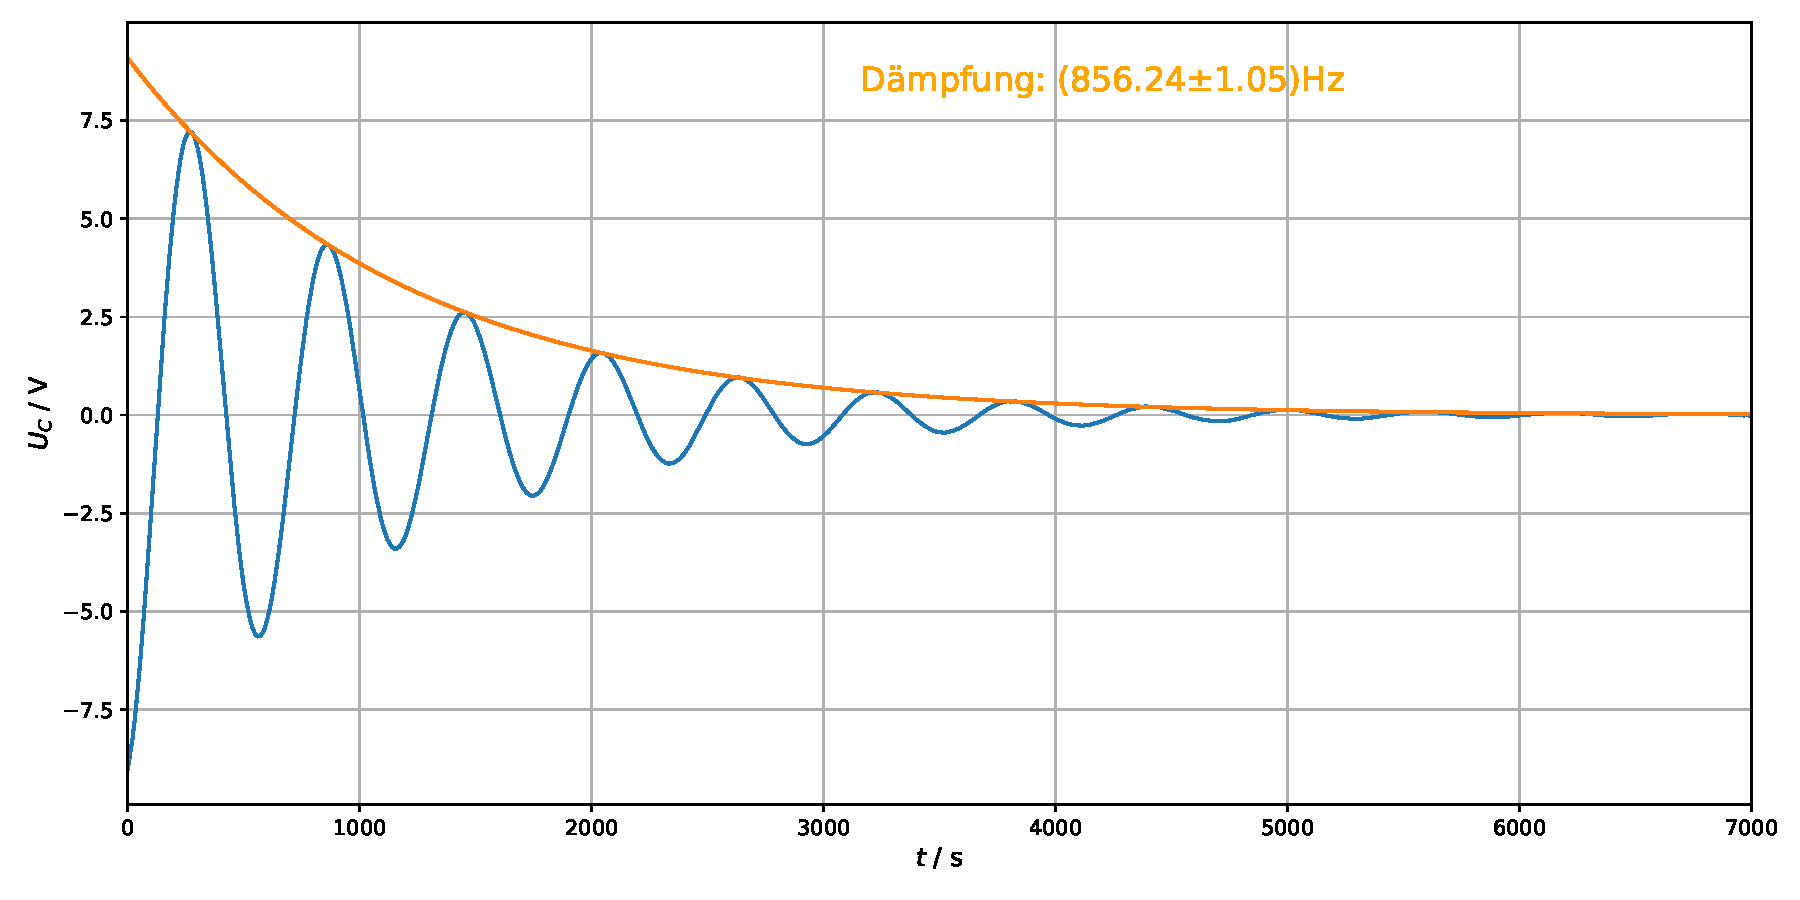
\includegraphics[width=\textwidth]{plots/einhuellend/exp_einhuellend3_2.pdf}
\caption{Mittels Python berechnete exponentiell Einhüllende für die zweite Messung des $10\,\Omega$ Widerstands.}
\label{abb:einhuellende1}
\end{figure}

Die berechneten Dämpfungen mittels Fit einer einhüllenden Exponentialfunktion um die Schwingung können aus Tabelle \ref{tab:daempfung2} abgelesen werden. Die Größe der systematischen Fehler liegt dabei unter 1\% der statistischen Fehler, so dass die systematischen Fehler vernachlässigt werden. Die Fehler der gewichteten Mittel sind die äußeren Fehler der drei Messungen. Für eine Messung mit dem $10\,\Omega$ Widerstand ist die Einhüllende in Abbildung \ref{abb:einhuellende1} geplotet. Im Anhang \ref{app:expein} befinden sich Einhüllende für jeweils eine Messung der übrigen Widerstände.


\begin{table}[H]
\centering
\begin{adjustbox}{width=\textwidth}
\begin{tabular}{c|cccc}
\multirow{2}{*}{Widerstand / $\Omega$} & \multicolumn{4}{c}{$\delta$ mit Exp-Einhüllender / Hz} \\
\cline{2-5}
& Messung 1 & Messung 2 & Messung 3 & Mittel\\
\hline
$1$ & $348.56 \pm 0.27$ & $324.45\pm 0.23$ & $325.60\pm 0.23$ & $331.32\pm 7.38$ \\
$5.1$ & $562.21 \pm 0.55$ & $574.88\pm 0.57$ & $575.29\pm 0.57$ & $570.61\pm 4.34$ \\
$10$ & $858.22 \pm 1.05$ & $856.24\pm 1.05$ & $849.17\pm 1.03$ & $854.48\pm 2.76$ \\
$20$ & $1409.89 \pm 2.51$ & $1417.40\pm 2.54$ & $1409.46\pm 2.51$ & $1412.21\pm 2.57$ \\
$47$ & $2995.46 \pm 13.28$ & $2891.72\pm 8.96$ & $2922.18\pm 12.57$ & $2923.66\pm 29.28$
\end{tabular}
\end{adjustbox}
\caption{Durch Anwendung der Pythonmethode \url{analyse.exp_einhuellende} bestimmte Dämpfungen.}
\label{tab:daempfung2}
\end{table}

Nun kann $\delta$ über $R$ aufgetragen und eine Regression durchgeführt werden. Dies ist sowohl für die Daten aus Tabelle \ref{tab:daempfung1} als auch aus Tabelle \ref{tab:daempfung2} in Abbildung \ref{abb:reg_Rdelta} dargestelt.

\begin{figure}[H]
\centering
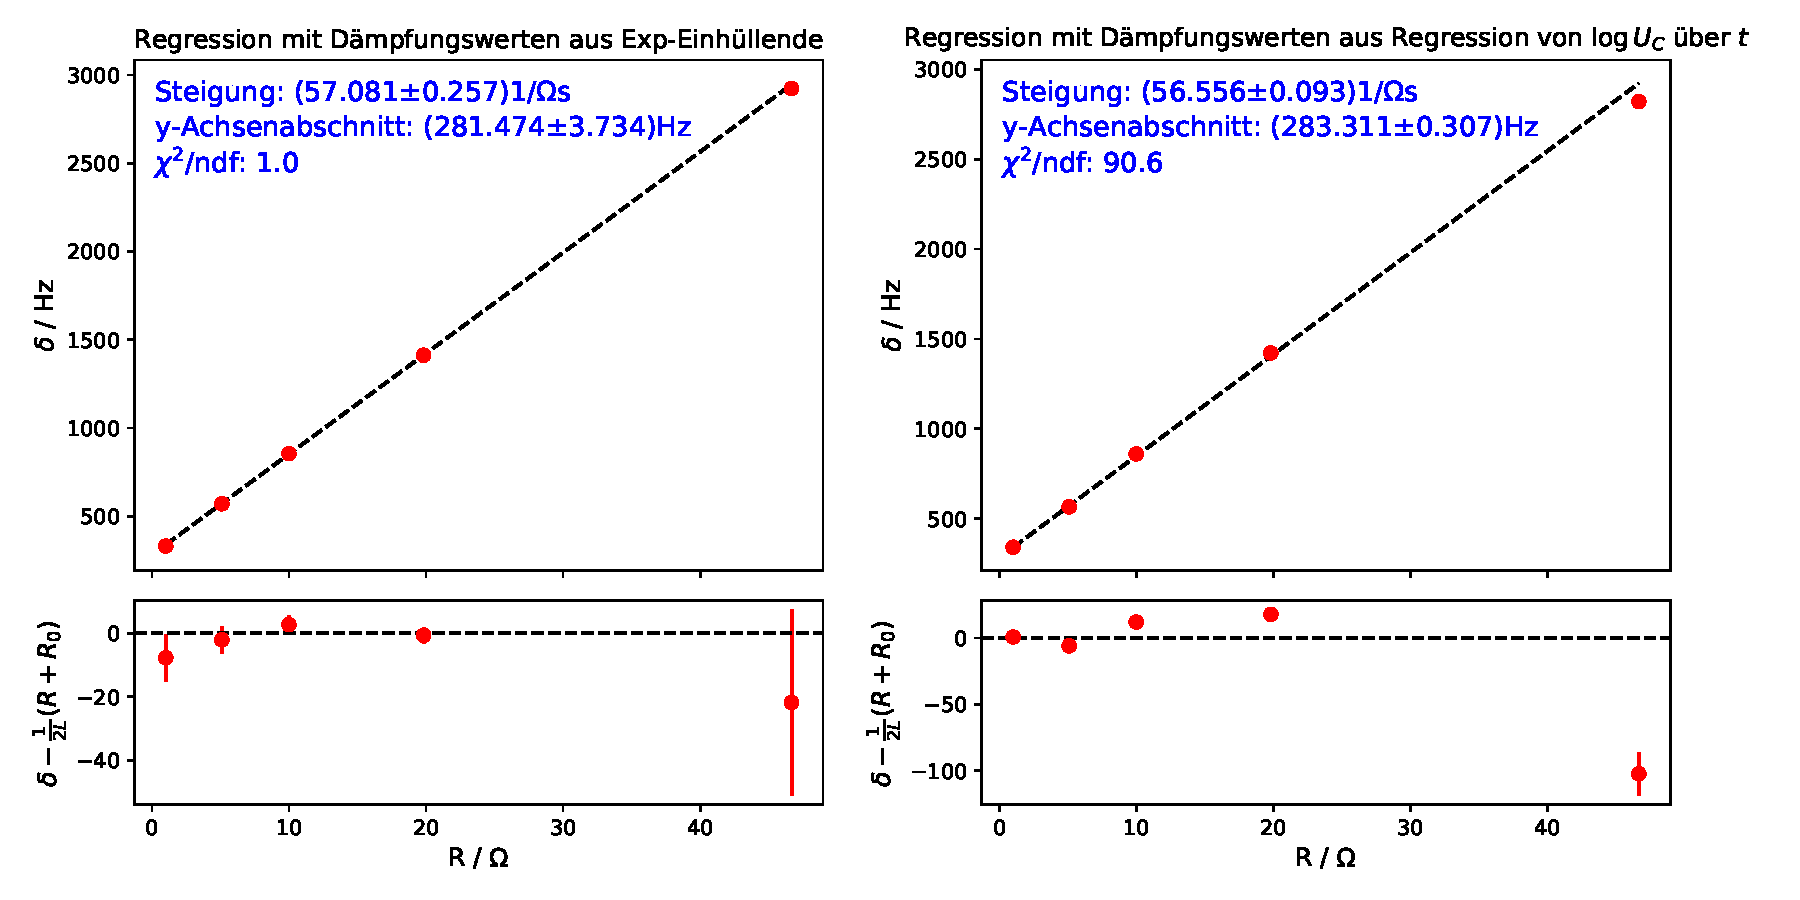
\includegraphics[width=\textwidth]{plots/reg_delR.pdf}
\caption{Regressionen von $\delta$ über R zur Bestimmung von L.}
\label{abb:reg_Rdelta}
\end{figure}

Die Daten, die mit den Einhüllenden berechnet wurden, liefern die bessere Regression und werden daher für die weitere Auswertung verwendet. Im Gegensatz zu den Frequenzen kann man hier nicht direkt an der Tabelle erkennen, welche Daten qualitativ besser sind. Ein Nachteil von den Dämpfungswerten aus der Methode \url{exp_einhuellende} sind die (verglichen mit den Regressions-Daten) großen Fehler, die aufgrund unterschiedlicher Ergebnisse in den einzelnen Messreihen entstehen. Mit der linken Regressiongerade $\text{reg}(R) = \Delta \cdot R + \alpha$ aus Abbildung \ref{abb:reg_Rdelta} folgt nun
\begin{align*}
R_0 &= \frac{\alpha}{\Delta r} = 4.93 \, \Omega 
\hspace{0.4cm} \text{ mit } \hspace{0.4cm}
\sigma_{R_0} = R_0 \sqrt{\left(\frac{\sigma_\alpha}{\alpha}\right)^2 + \left(\frac{\sigma_\Delta}{\Delta}\right)^2} = 0.07 \, \Omega 
\intertext{und} 
L &= \frac{1}{2\Delta} = 8.759 \, \mathrm{mH} 
\hspace{0.4cm} \text{ mit } \hspace{0.4cm}
\sigma_{L} = \frac{\sigma_\Delta}{\Delta^2} = 0.079 \, \mathrm{mH}.
\end{align*}

\begin{figure}[H]
\centering
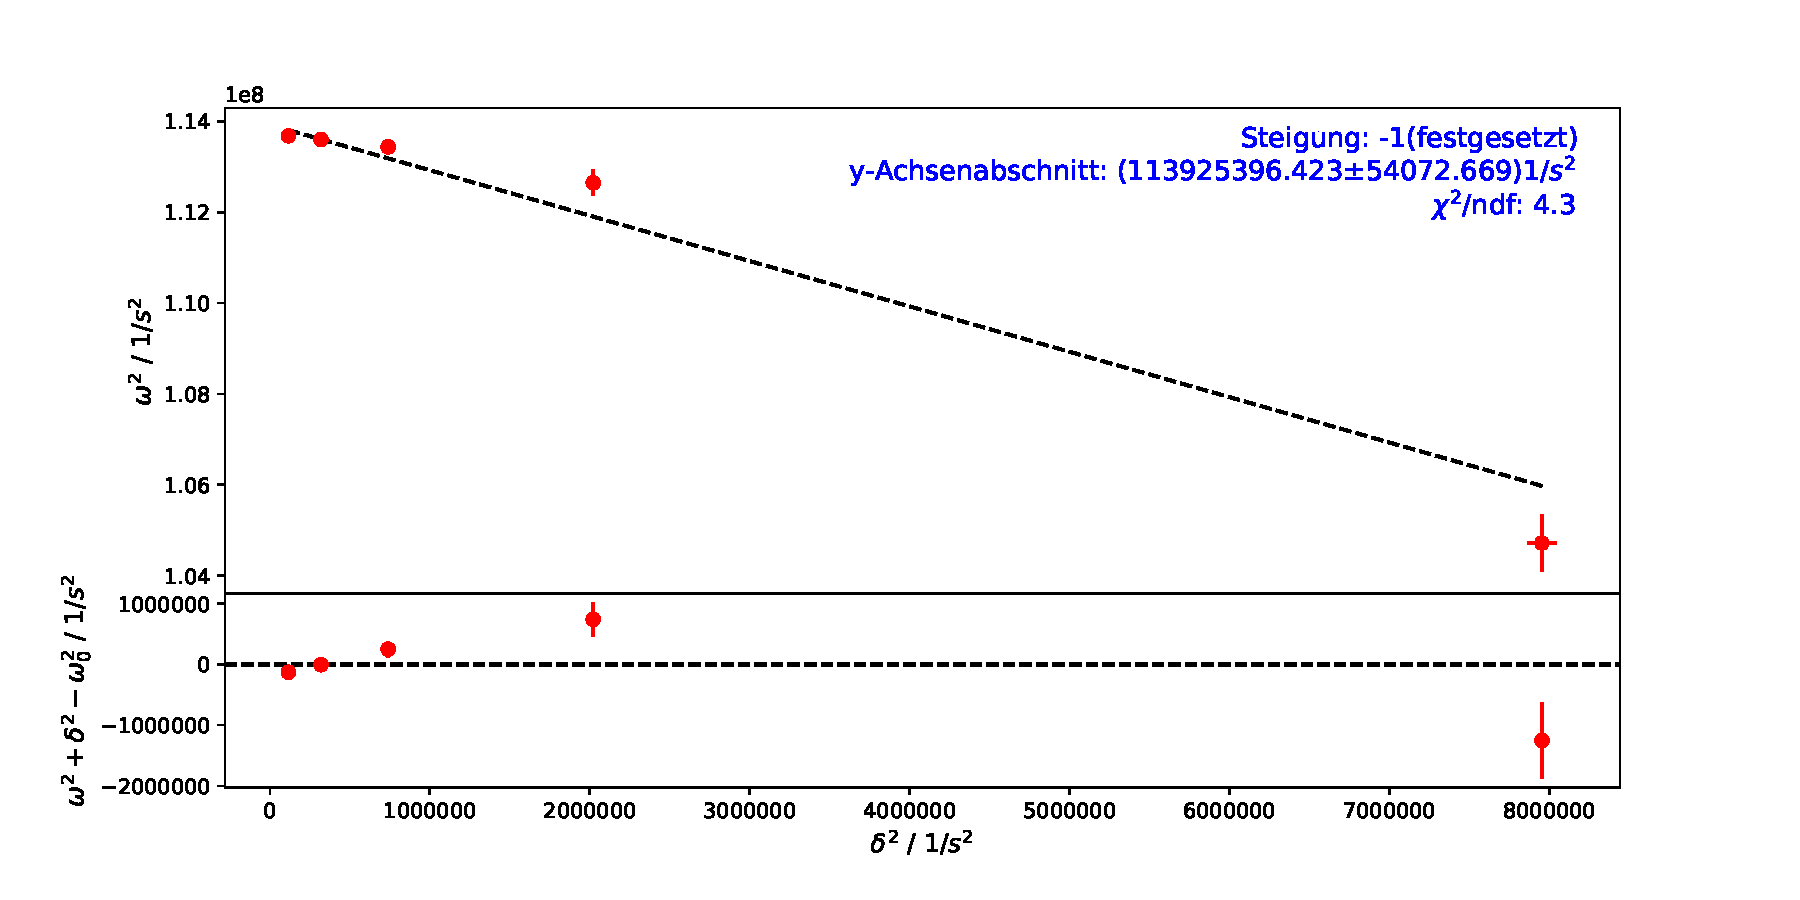
\includegraphics[width=\textwidth]{plots/reg_delomega.pdf}
\caption{Regression von $\omega^2$ über $\delta^2$ zur Bestimmung von $\omega_0$.}
\label{abb:reg_delomega}
\end{figure}


Mit diesen Ergebnissen liefert eine Regression von $\omega^2$ über $\delta^2$, die in Abbildung \ref{abb:reg_delomega} gezeigt ist, die Grundfrequenz $\omega_0 = (10673.58\pm 2.53)\,$Hz, d.h. $f_0 = (1698.75\pm 0.40)\,$Hz, und eine Kapazität von $C = \frac{1}{L\omega_0^2} = (1.002\pm 0.009)\,\mu$F. 

\begin{figure}[h]
\centering
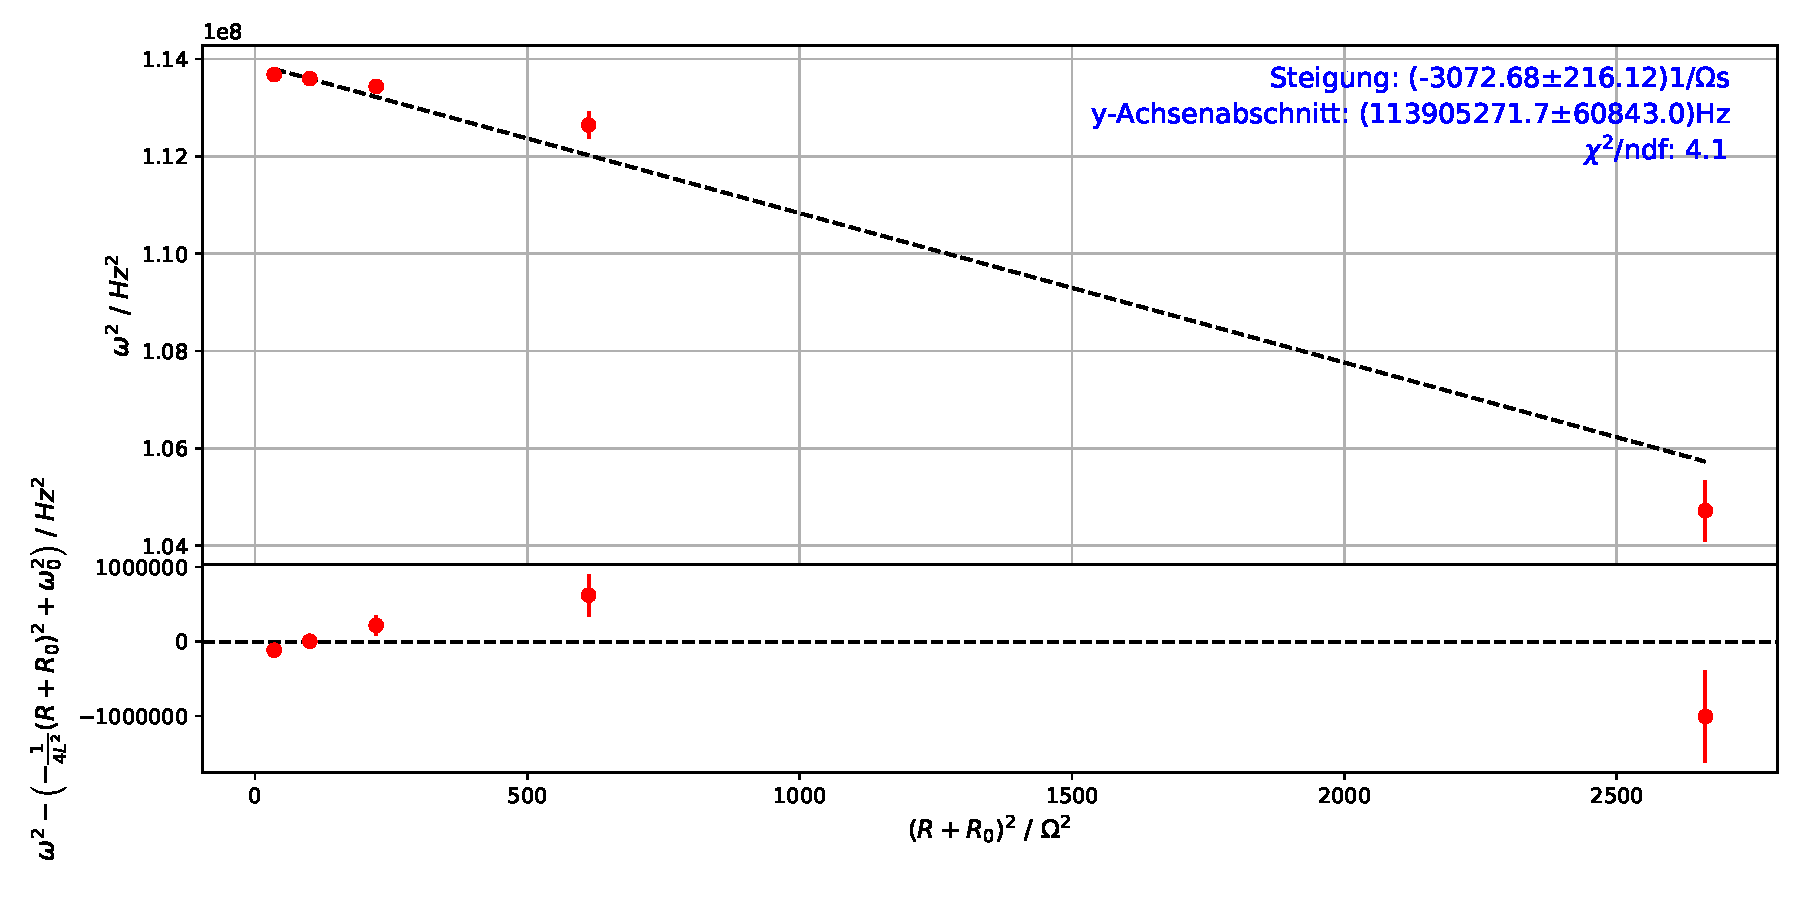
\includegraphics[width=\textwidth]{plots/reg_Rome.pdf}
\caption{Regression von $\omega^2$ über $(R+R_0)^2$ zur Bestimmung von $\omega_0$ und $L$.}
\label{abb:reg_Rome}
\end{figure}

Alternativ kann auch der Restwiderstand $R_0 = (4.93\pm 0.07)\,\Omega$ aus der Regression \ref{abb:reg_Rdelta} verwendet werden, um eine Regression von $\omega^2$ über $(R+R_0)^2$ anzufertigen. Aus \ref{eq:korrektur} folgt nämlich
$$\omega^2 = \omega_0^2 - \frac{1}{4L^2} R_{\text{Ges}}^2\text{.}$$
Somit kann $\omega_0$ als Wurzel des y-Achsenabschnitts und $L$ aus der Steigung bestimmt werden. Diese Regression ist in Abbildung \ref{reg_Rome} dargestellt und liefert $\omega_0 = (10672.64\pm 2.85)\,$Hz, d.h. $f_0 = (1698.60\pm0.45)\,$Hz und $L = (9.020\pm0.317)\,$mH. Dies wiederum ergibt eine Kapazität von $C = \frac{1}{L\omega_0^2} = (0.973\pm 0.034)\,\mu$F.



\subsubsection{Aperiodischer Grenzfall und Kriechfall}

\begin{figure}[H]
\centering
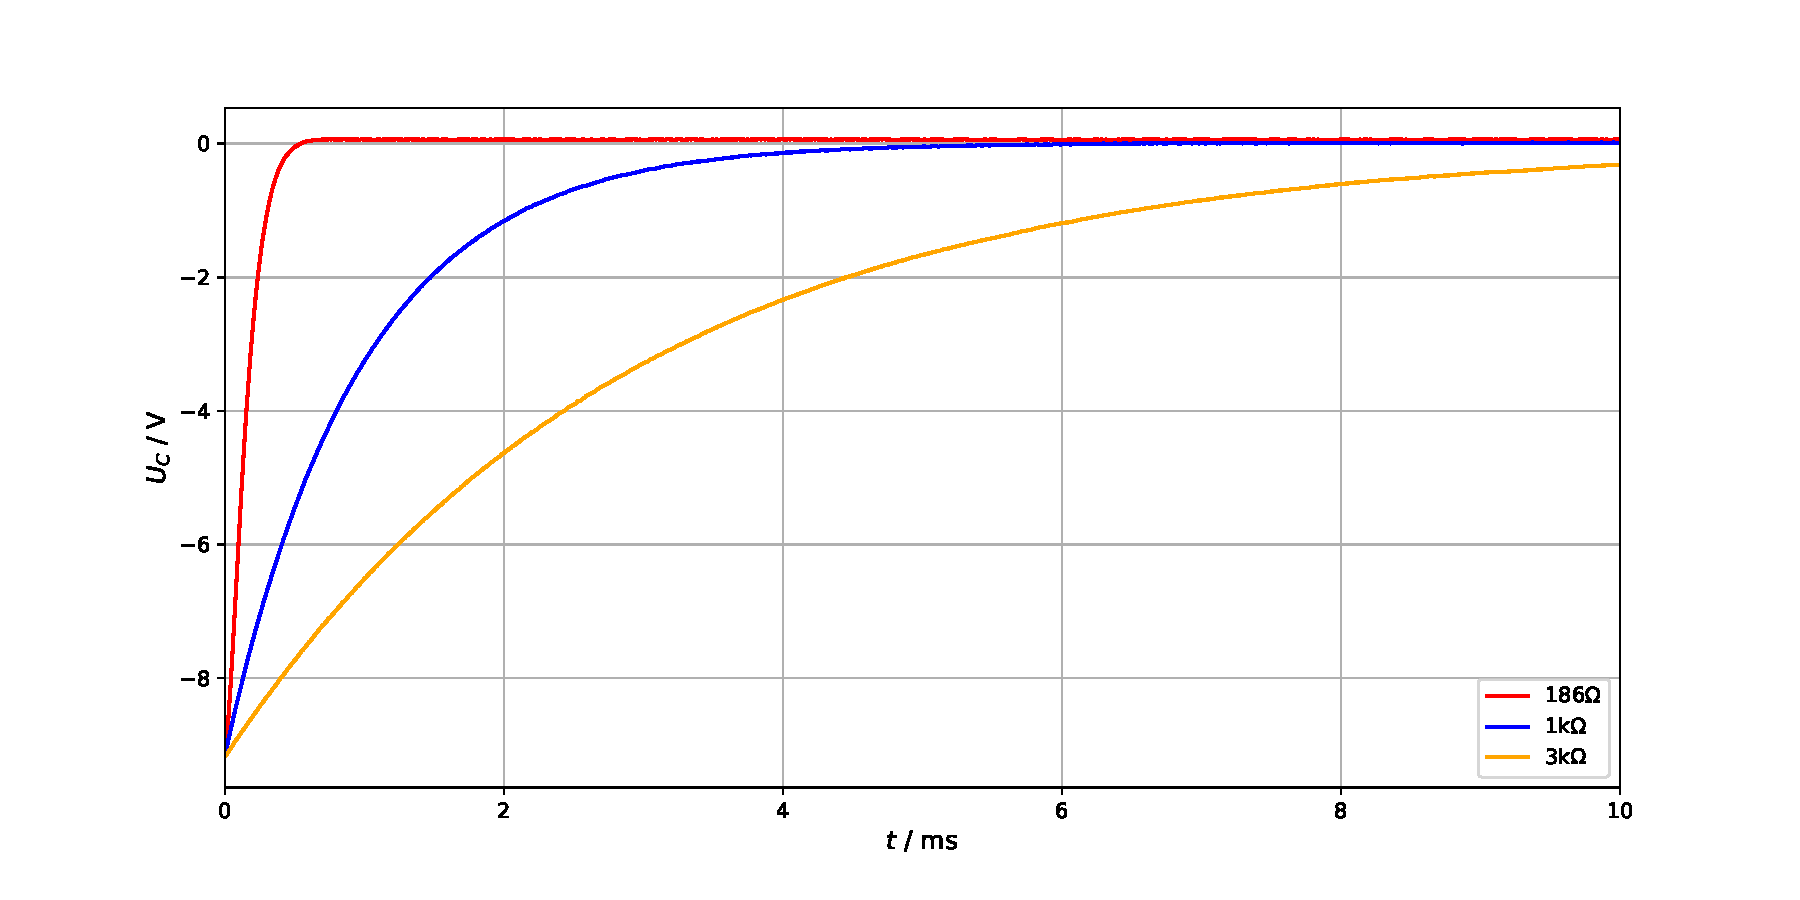
\includegraphics[width=\textwidth]{plots/rohdaten_kriech.pdf}
\caption{Visualisierung der Messreihen des aperiodischen Grenz- und Kriechfalls}
\label{abb:rohkriech}
\end{figure}

Aus der vorangegangen Analyse der Messreihen des Schwingfalls erhalten wir einen Restwiderstand von $R_0 = (4.93\pm0.07)\, \Omega$. Zusammen mit dem Widerstand des Potentiometers, der im aperiodischen Grenzfall $(186\pm 1)\, \Omega)$ beträgt, ergibt sich der Gesamtwiderstand $R_{\text{Ges}} = (190.93 \pm 1)\, \Omega$. Mit der gemessenen Kapazität und Induktivität aus der Versuchsdurchführung erhält man einen erwarteteten Widerstand $R_{ap}$ von
$$ R_{ap} = 2\sqrt{\frac{L}{C}} = (191.27 \pm 0.11) \,\Omega.$$
Dies deckt sich im Rahmen der Unsicherheiten mit dem gemessenen Widerstand $R_{Ges}$. In Abbildung \ref{abb:rohkriech} kann man zudem qualitativ gut erkennen, wie ein zunehmender Widerstand, die Entladezeit des Kondensators erhöht.


\subsection{Fazit}

Bei der Regression von $\delta$ über $R$ erhalten wir eine Induktivität von $L = (8.759 \pm 0.079) \,$mH und damit eine relative Abweichung von
$$\frac{|L-L_g|}{\sqrt{\sigma_L^2 + \sigma_{L_g}^2}} \approx 1.89$$
zum gemessenen Wert $L_g = (9.00 \pm 0.01)\,$mH. Dies ist angesichts der mäßigen Modellanpassungen akzeptabel. Entsprechend bekommt man hier natürlich eine etwas zu große Kapazität von $C = (1.002 \pm 0.009)\, \mu$F im Vergleich zum gemessenen Wert $C_g = (0.9842 \pm 0.0002)\,\mu$F mit einer relativen Abweichung von etwa 1.98. Bei der alternativen Regression von $\omega^2$ über $(R+R_0)^2$ ergeben sich hingegen passendere Werte von $L = (9.020 \pm 0.317) \,$mH und $(0.973 \pm 0.034)\,\mu$F, wobei die Fehler hier deutlich größer sind. Außerdem konnte man qualitativ sehen, welchen Einfluss die zunehmende Dämpfung auf den Einschwingvorgang hat und Schwing-, Kriech- und den aperiodischen Grenzfall beobachten. Bei dem aperiodischen Grenzfall stimmt gemessener und erwarteter Widerstand gut überein. Nebenbei konnten wir den Restwiderstand der Schaltung $R_0 = (4.93 \pm 0.07) \,\Omega$ auf etwa 1.5 \% genau bestimmen. 



\newpage
\section{Gekoppelte LC-Schwingkreise}


\subsection{Versuchsbeschreibung}

In diesem Versuch werden zwei Schwingkreise induktiv miteinander gekoppelt. Speziell werden hier die beiden Fundamentalschwingungen bei gleichsinniger und gegensinniger Anregung und eine Schwebung aufgezeichnet.

\begin{figure}[H]
\centering
\begin{tikzpicture}
% Linke Schwingkreise
\draw (0,0.2) -- (-1,0.2) to [rmeterwa, t=$U_1$] (-1,1.8) -- (0,1.8);
\draw (0.8,0) node[ocirc]{} -- (0,0) to [C, a=$C$] (0,2) -- (2,2) to [cute inductor, a=$L$] (2,0) -- (1.2,0) node[ocirc]{};
\draw (3.55,0) node[ocirc]{} -- (2.75,0) to [cute inductor, a=$L$] (2.75,2) -- (4.75,2) to[C, a=$C$] (4.75,0) -- (3.95,0) node[ocirc]{};
\draw (4.75,0.2) -- (5.75,0.2) to [rmeterwa, t=$U_2$] (5.75,1.8) -- (4.75,1.8);
\draw (2,0) to [normal open switch] (2,-1) -- (0,-1) -- (0,0);
\draw (2.75,0) to [normal open switch] (2.75,-1) -- (4.75,-1) -- (4.75,0);
\draw[dashed, thin] (2.15,-0.5) -- (2.85,-0.5); 


% Rechte Schwingkreise
\draw (8,0.2) -- (7,0.2) to [rmeterwa, t=$U_1$] (7,1.8) -- (8,1.8);
\draw (8.8,0) node[ocirc]{} -- (8,0) to [C, a=$C$] (8,2) -- (10,2) to [cute inductor, a=$L$] (10,0) -- (9.2,0) node[ocirc]{};
\draw (11.55,0) node[ocirc]{} -- (10.75,0) to [cute inductor, a=$L$] (10.75,2) -- (12.75,2) to[C, a=$C$] (12.75,0) -- (11.95,0) node[ocirc]{};
\draw (12.75,0.2) -- (13.75,0.2) to [rmeterwa, t=$U_2$] (13.75,1.8) -- (12.75,1.8);
\draw (10,0) to [normal open switch] (10,-1) -- (8,-1) -- (8,0);
\draw (10.75,0) to [normal open switch] (10.75,-1) -- (12.75,-1) -- (12.75,0);
\draw[dashed, thin] (10.15,-0.5) -- (10.85,-0.5); 

\end{tikzpicture}
\caption{Fundamentalschwingungen der gekoppelten Schwingkreise bei gleichsinniger (links) und gegensinniger Anregung (rechts)}
\end{figure}

Bei überbrückter Spannungsquelle gelten für den gekoppelten Schwingkreis die folgenden Differentialgleichungen 
\begin{align*}
\ddot I_1 + k \ddot I_2 + \frac{1}{LC}I_1 &= 0 \\
\ddot I_2 + k \ddot I_1 + \frac{1}{LC}I_2 &= 0
\end{align*}
Dabei bezeichnet $k \in (0,1)$ die Kopplung der beiden Schwingkreise. 
Mit den sogenannten \textit{Fundamentalströmen} $I_+ = I_1 + I_2$ und $I_- = I_1 - I_2$ erhält man durch Addition bzw. Subtraktion der obigen Gleichungen und anschließendem Umformen
\begin{align*}
\ddot I_+ + \frac{1}{LC(1+k)} I_+ = 0 \\
\ddot I_- + \frac{1}{LC(1-k)} I_- = 0
\end{align*}
Daraus ergeben sich harmonische Schwingungen mit den Kreisfrequenzen 
$$\omega_+ = \frac{\omega_0}{\sqrt{1+k}} \hspace{0.2cm} \text{ und } \hspace{0.2cm} \omega_- = \frac{\omega_0}{\sqrt{1+k}}.$$
Dabei ist $\omega_0 = \frac{1}{\sqrt{LC}}$ die Kreisfrequenz der ungekoppelten Schwingung. Mithilfe der Fundamentalschwingungen lässt sich dann der Kopplungsgrad bestimmen
$$k = \frac{f_-^2 - f_+^2}{f_-^2 + f_+^2}.$$
Bei Messung einer Schwebung mit Schwebungsfrequenz $f_s$ und Frequenz der gekoppelten Schwingung $f_k$ kann man die Fundamentalschwingungen gemäß
$$f_k = \frac{f_- + f_+}{2} \hspace{0.2cm} \text{ und } \hspace{0.2cm} f_s = \frac{f_- - f_+}{2}$$
bestimmen. Aufgrund der unvermeidbaren Dämpfung der beiden Schwingkreise sind die Extrema des einen Schwingkreises gegen die Nulldurchgänge des anderen verschoben. Für Kopplungen $k < 0.2$ gilt näherungsweise für die zeitliche Verschiebung

\begin{equation}\label{eq:delta_t}
\Delta t \approx \frac{1}{\omega_s} \left( \frac{\pi}{2} - \arctan\left(  \frac kR \sqrt{\frac LC}\right) \right)
\end{equation}



\subsection{Schwebung}


\subsubsection{Versuchsaufbau}

\begin{figure}[H]
\centering
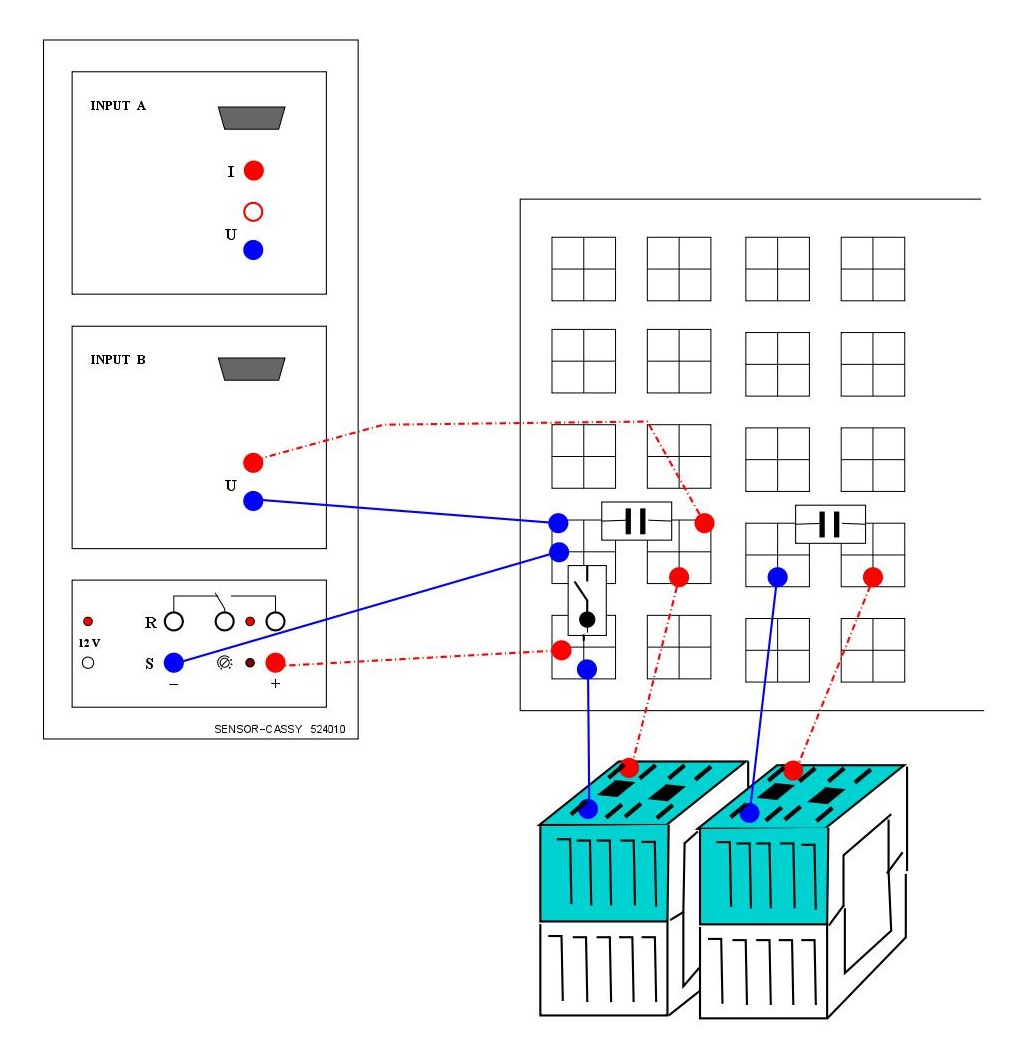
\includegraphics[width=0.6\textwidth]{bilder/aufbau_schwebung.jpg}
\caption{Aufbau zur Erzeugung einer Schwebung}
\label{abb:aufbau_schweb}
\end{figure}

Zur Erzeugung einer Schwebung wird nur einer der beiden Schwingkreise angeregt. Die Schwingkreise werden gemäß Abbildung \ref{abb:aufbau_schweb} auf der Rastersteckplatte aufgebaut. Als Schalter dient dabei ein Taster. Im ersten Schwingkreis werden Kondensator und Spule aus dem ersten Versuch verwendet. Für den zweiten Schwingkreis werden baugleiche Teile benutzt.


\subsubsection{Versuchsdurchführung}

Kondensator 1 wird mit $U_0 = 9.5 \, \mathrm V$ aufgeladen. Die Spannung am ersten Kondensator $U_1$ wird im Eingang A des ersten Sensor-CASSYs und die Spannung am zweiten Kondensator $U_2$ wird im Eingang A des zweiten Sensor-CASSYs gemessen. Für die Messungen werden folgende Messparameter verwendet:

\begin{enumerate}[-]
\setlength{\itemsep}{-5pt} 
\item Messart: automatische Aufnahme
\item Messbereich: $\pm$10 V
\item Messintervall: $10\,\mu$s 
\item Messungen: $8000$
\item Messzeit: $80\,$ms
\end{enumerate}

Die Messung wird dabei durch einen Trigger auf die fallende Flanke von $U_1$ bei 6.7 V gestartet. Es werden Schwebungen in drei verschiedenen Konfigurationen aufgezeichnet. Bei Schwebung 1 befinden sich die Spulen direkt aneinander. Bei Schwebung 2 haben die Spulen einen Abstand von etwa 5 cm und bei Schwebung 3 werden die Spulen direkt aneinander auf einen Eiskern gepackt. Bei einer Messung mit einer LCR-Messbrücke von Telemeter Electronic ergaben sich für die Bauteile die folgenden Werte:

\begin{table}[H]
\centering
\begin{tabular}{c|c|c}
Schwingkreis & Kapazität / nF & Induktivität / mH\\
\hline
1 & $984.2 \pm 0.2$ & $9.03 \pm 0.01$ \\
2 & $980.1 \pm 0.1$ & $9.00 \pm 0.01$
\end{tabular}
\end{table} 

Die Fehler wurden dabei anhand der Fluktuation des angezeigten Wertes geschätzt.

\subsubsection{Versuchsauswertung}

Die Rohdaten zu Schwebung 1 sind in Abbildung \ref{abb:schwebung_roh} beispielhaft zu sehen.

\begin{figure}[H]
\centering
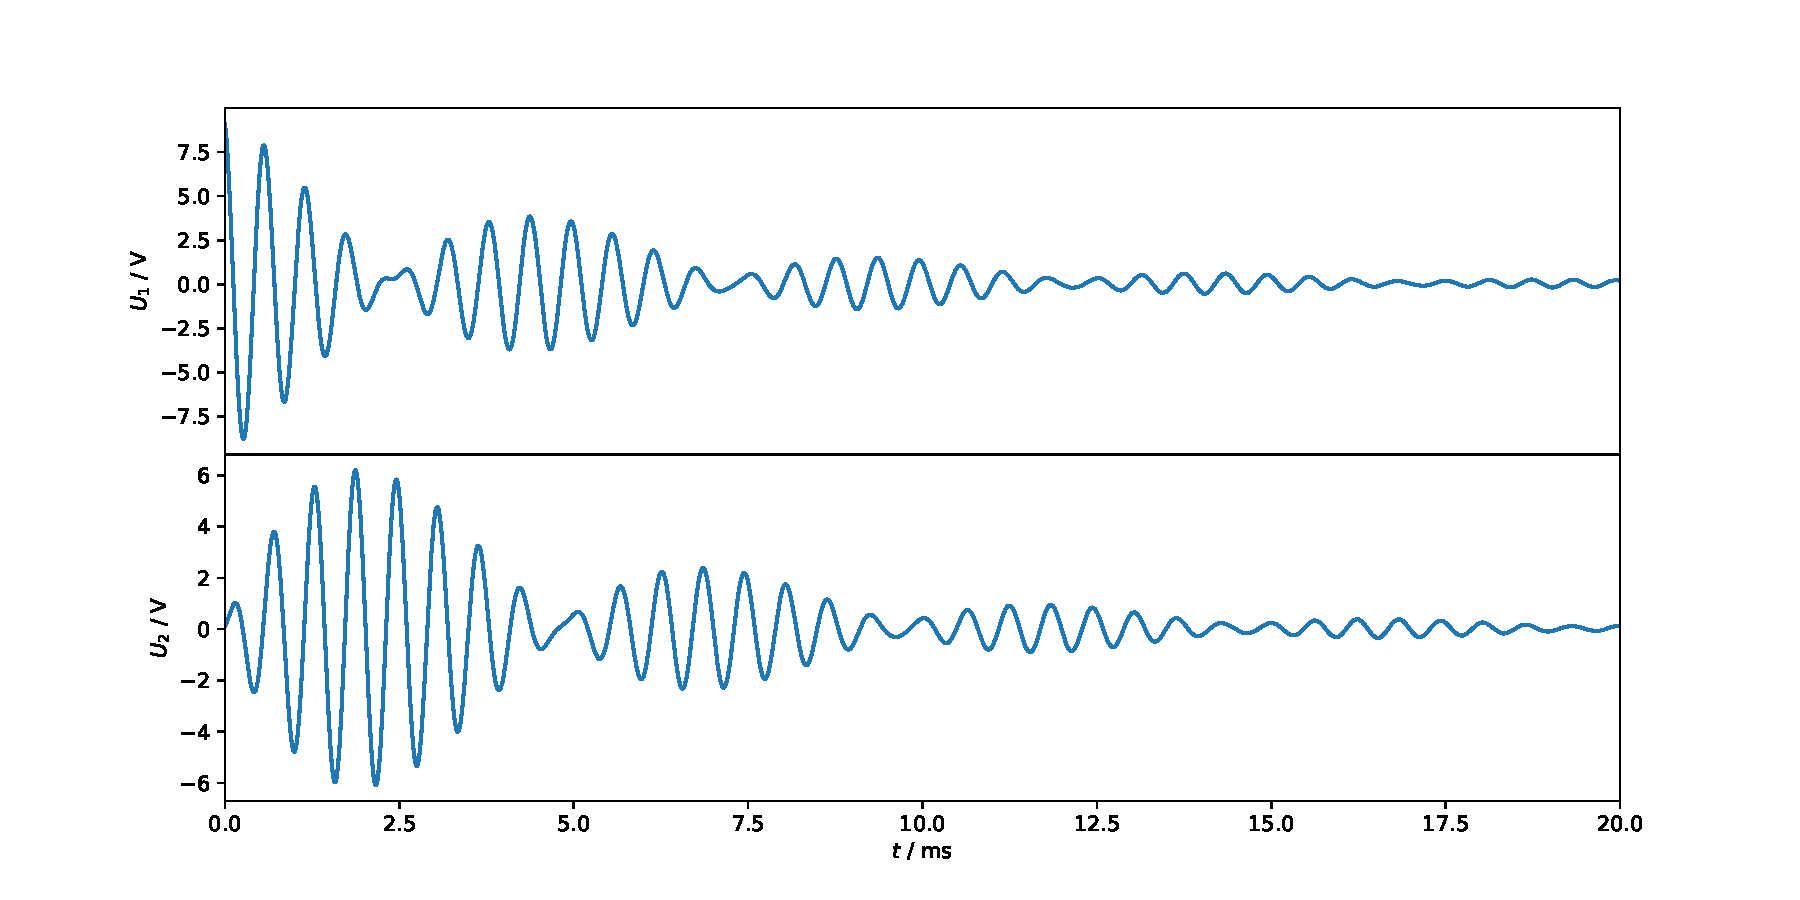
\includegraphics[width=\textwidth]{plots/schwebung_roh.pdf}
\caption{Rohdaten der Schwebung}
\label{abb:schwebung_roh}
\end{figure}

Da sich die Periodendauer der Schwebung bei den beiden anderen Schwebungen garnicht anhand der Schwebungsmaxima bestimmen lässt, wird ausschließlich eine Auswertung mittels FFT vorgenommen. Die Frequenzspektren für alle drei Konfigurationen sind in Abbildung \ref{abb:FFT_schwebung} zu sehen. Diese wurden aus der Spannung am ersten Kondensator berechnet.

\begin{figure}
\centering
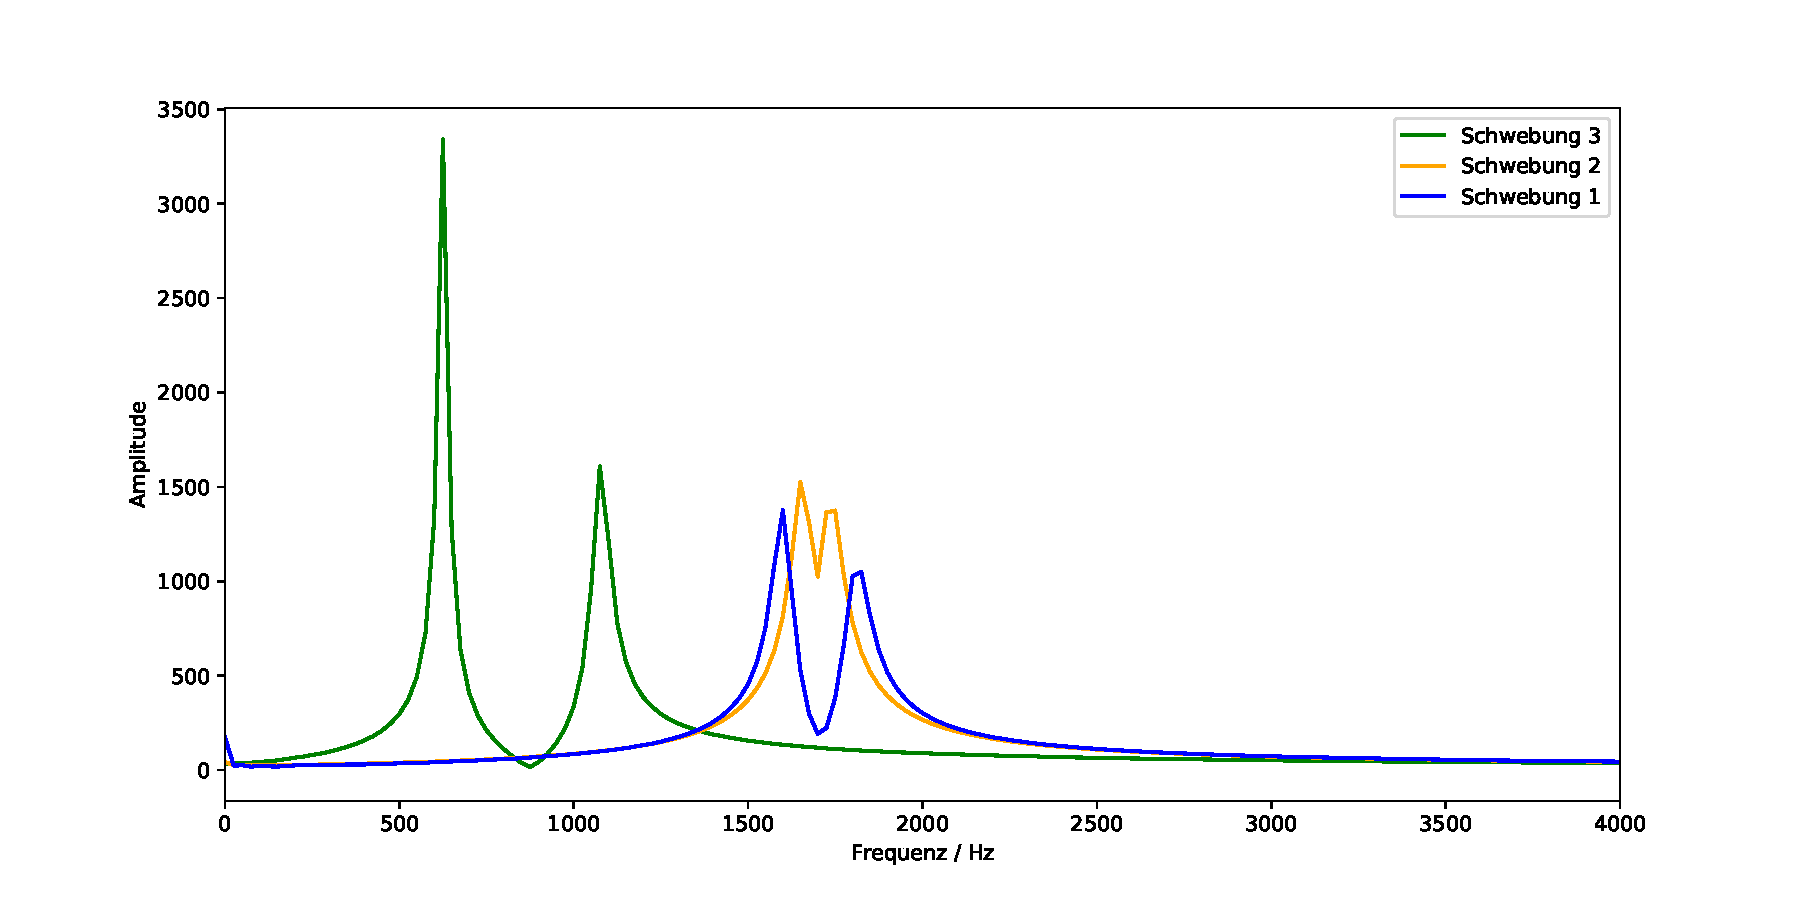
\includegraphics[width=\textwidth]{plots/FFT_schwebungen.pdf}
\caption{Frequenzspektren der drei Schwebungen}
\label{abb:FFT_schwebung}
\end{figure}

Man erkennt gut, dass mit zunehmender Dämpfung die Peaks weiter auseinander liegen und der Mittelwert der Peaks sich zu kleineren Frequenzen verschiebt. Mit der Peak-Schwerpunktmethode ergeben sich die Frequenzen in Tabelle \ref{tab:freq_schweb}. Als Fehler wird dabei die Frequenzdifferenz zwischen Argument-Maximum und Peakschwerpunkt verwendet.

\begin{table}[H]
\centering
\begin{tabular}{c|c|c}
Schwebung & $f_+$ / Hz & $f_-$ / Hz \\
\hline
1 & $1598.65 \pm 0.95$ & $1832.1 \pm 7.5$ \\
2 & $1639 \pm 11$ & $1727 \pm 23$ \\
3 & $631.8 \pm 6.9$ & $1094 \pm 19$
\end{tabular}
\caption{Frequenzen aus FFT}
\label{tab:freq_schweb}
\end{table}

Die Spannung am zweiten Kondensator liefert hier identische Werte. Mithilfe der Frequenzen lassen sich nun die Kopplungsgrade der drei Konfigurationen berechnen. Es gilt
$$k = \frac{f_-^2 - f_+^2}{f_-^2 + f_+^2}.$$
Mittels Gaußscher Fehlerfortpflanzung lässt sich der Fehler auf $k$ zu
$$\sigma_k = \frac{4f_-f_+}{(f_-^2+f_+^2)^2} \sqrt{f_+^2 \sigma_{f_-}^2 + f_-^2 \sigma_{f_+}^2}$$
bestimmen. Es ergeben sich die Werte in Tabelle \ref{tab:kopplung}.

\begin{table}[H]
\centering
\begin{tabular}{c|c}
Schwebung & $k$ \\
\hline
1 & $0.1355 \pm 0.0041$ \\
2 & $0.0522 \pm 0.0146$ \\
3 & $0.4999 \pm 0.0155$
\end{tabular}
\caption{Berechnete Kopplungsgrade}
\label{tab:kopplung}
\end{table}

Wir wollen nun noch überprüfen, ob die erwartete Zeitverschiebung aus Gleichung \ref{eq:delta_t} zutrifft. Die Beziehung gilt dabei nur für die Schwebungen 1 und 2. Da sich bei Schwebung 2 die Verschiebung nicht ablesen lässt, werten wir ausschließlich Schwebung 1 aus. Es lassen sich hier zwei Maxima/Nulldurchgänge auswerten. Abbildung \ref{abb:delta_t_bsp} veranschaulicht das Ablesen der Zeitpunkte und den Ablesefehler. 

\begin{figure}[H]
\centering
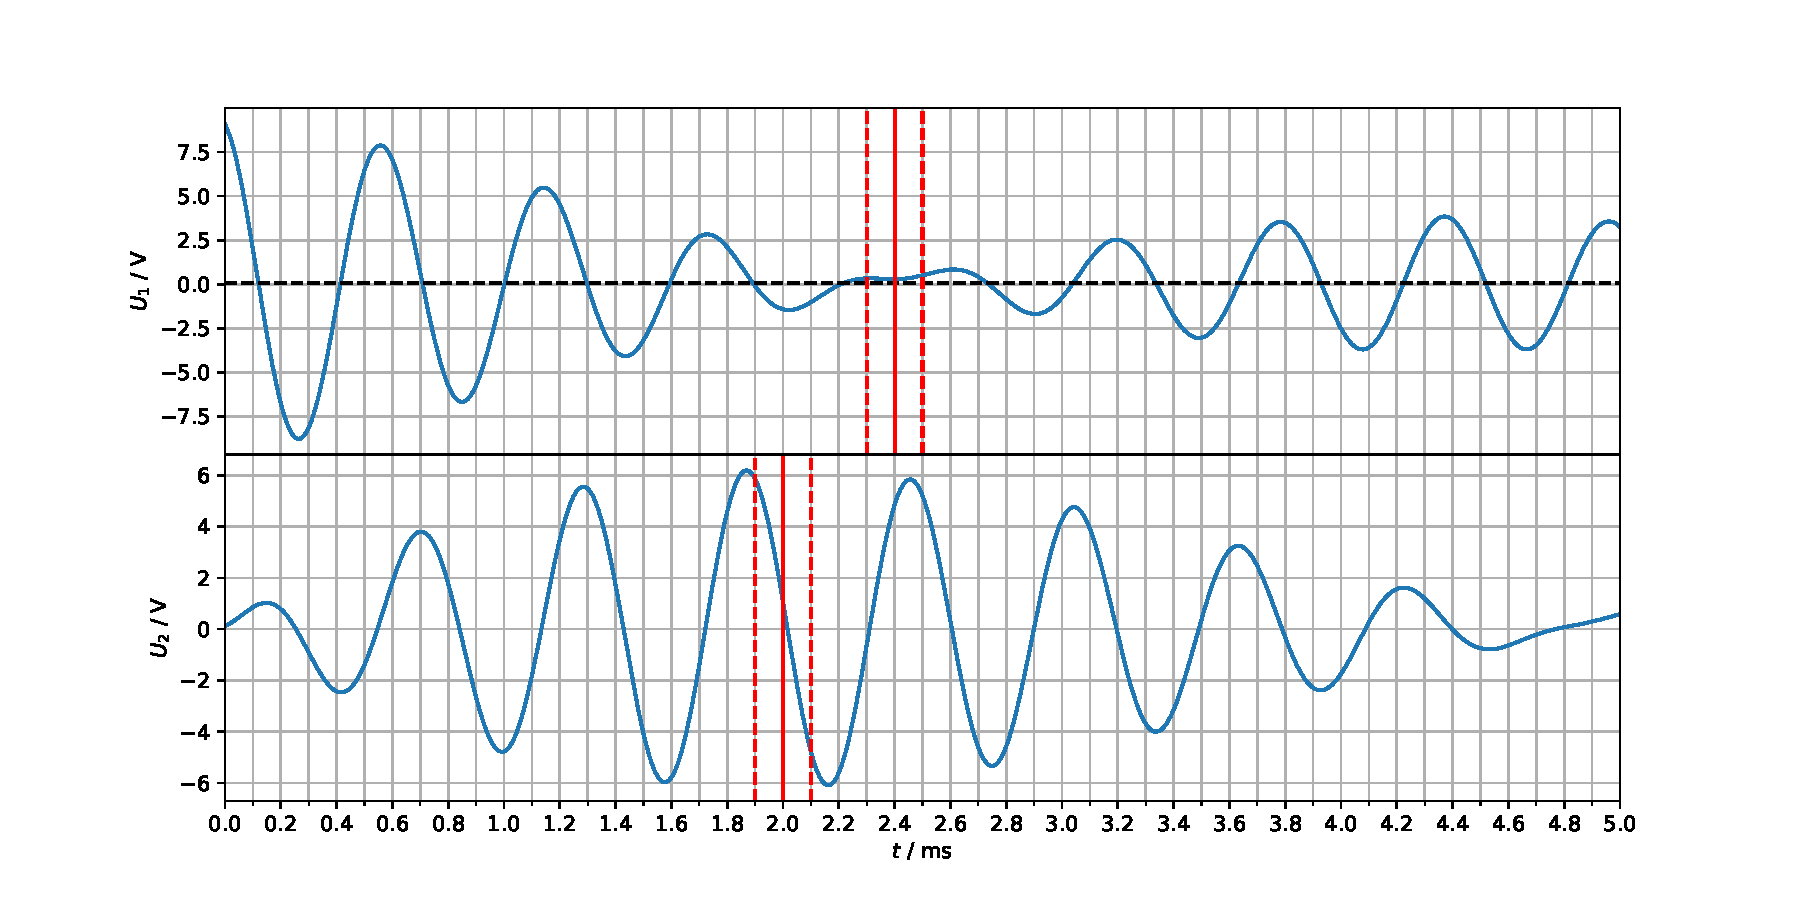
\includegraphics[width=\textwidth]{plots/delta_t_bsp.pdf}
\caption{Bestimmung der Nulldurchgänge/Maxima}
\label{abb:delta_t_bsp}
\end{figure}

Die abgelesenen Zeitpunkte sind in Tabelle \ref{tab:delta_t_zeiten} aufgeführt.

\begin{table}[H]
\centering
\begin{tabular}{c|c|c}
& $t_1$ / ms & $t_2$ / ms \\
\hline
Nulldurchgang $U_1$ & $2.4 \pm 0.1$ & $7.3 \pm 0.1$ \\
Maximum $U_2$ & $2.0 \pm 0.1$ & $6.9 \pm 0.1$
\end{tabular}
\caption{Abgelesene Zeitpunkte der Nulldurchgänge/Maxima}
\label{tab:delta_t_zeiten}
\end{table}

Nach Differenzbildung und gewichteter Mittelung ergibt sich mit dem inneren Fehler $\Delta t = (0.4 \pm 0.1) \, \mathrm{ms}$. Zum Vergleich berechnen wir die erwartete Zeitverschiebung
$$\Delta t_e \approx 0.495 \, \mathrm{ms}.$$
Dabei wurde für den Widerstand der Wert des Restwiderstandes aus dem ersten Versuch verwendet. Die abgelesene Verschiebung stimmt also innerhalb der Unsicherheiten mit der Erwartung überein.

\subsubsection{Fazit}

In diesem Versuch konnten einige qualitative Aussagen bestätigt werden. Zum einen konnte man sehen, dass die Peaks im Frequenzspektrum mit zunehmender Dämpfung zu kleineren Frequenzen verschoben sind und weiter auseinander liegen. Zudem konnte auch die erwartete Zeitverschiebung zwischen den Nulldurchgängen des einen und den Extrema des anderen Schwingkreises bestätigt werden. Nebenbei wurden die Kopplungsgrade $k$ für die erste und dritte Schwebung auf etwa 3 \% genau bestimmt.



\subsection{Fundamentalschwingungen}


\subsubsection{Versuchsaufbau}

\begin{figure}[H]
\centering
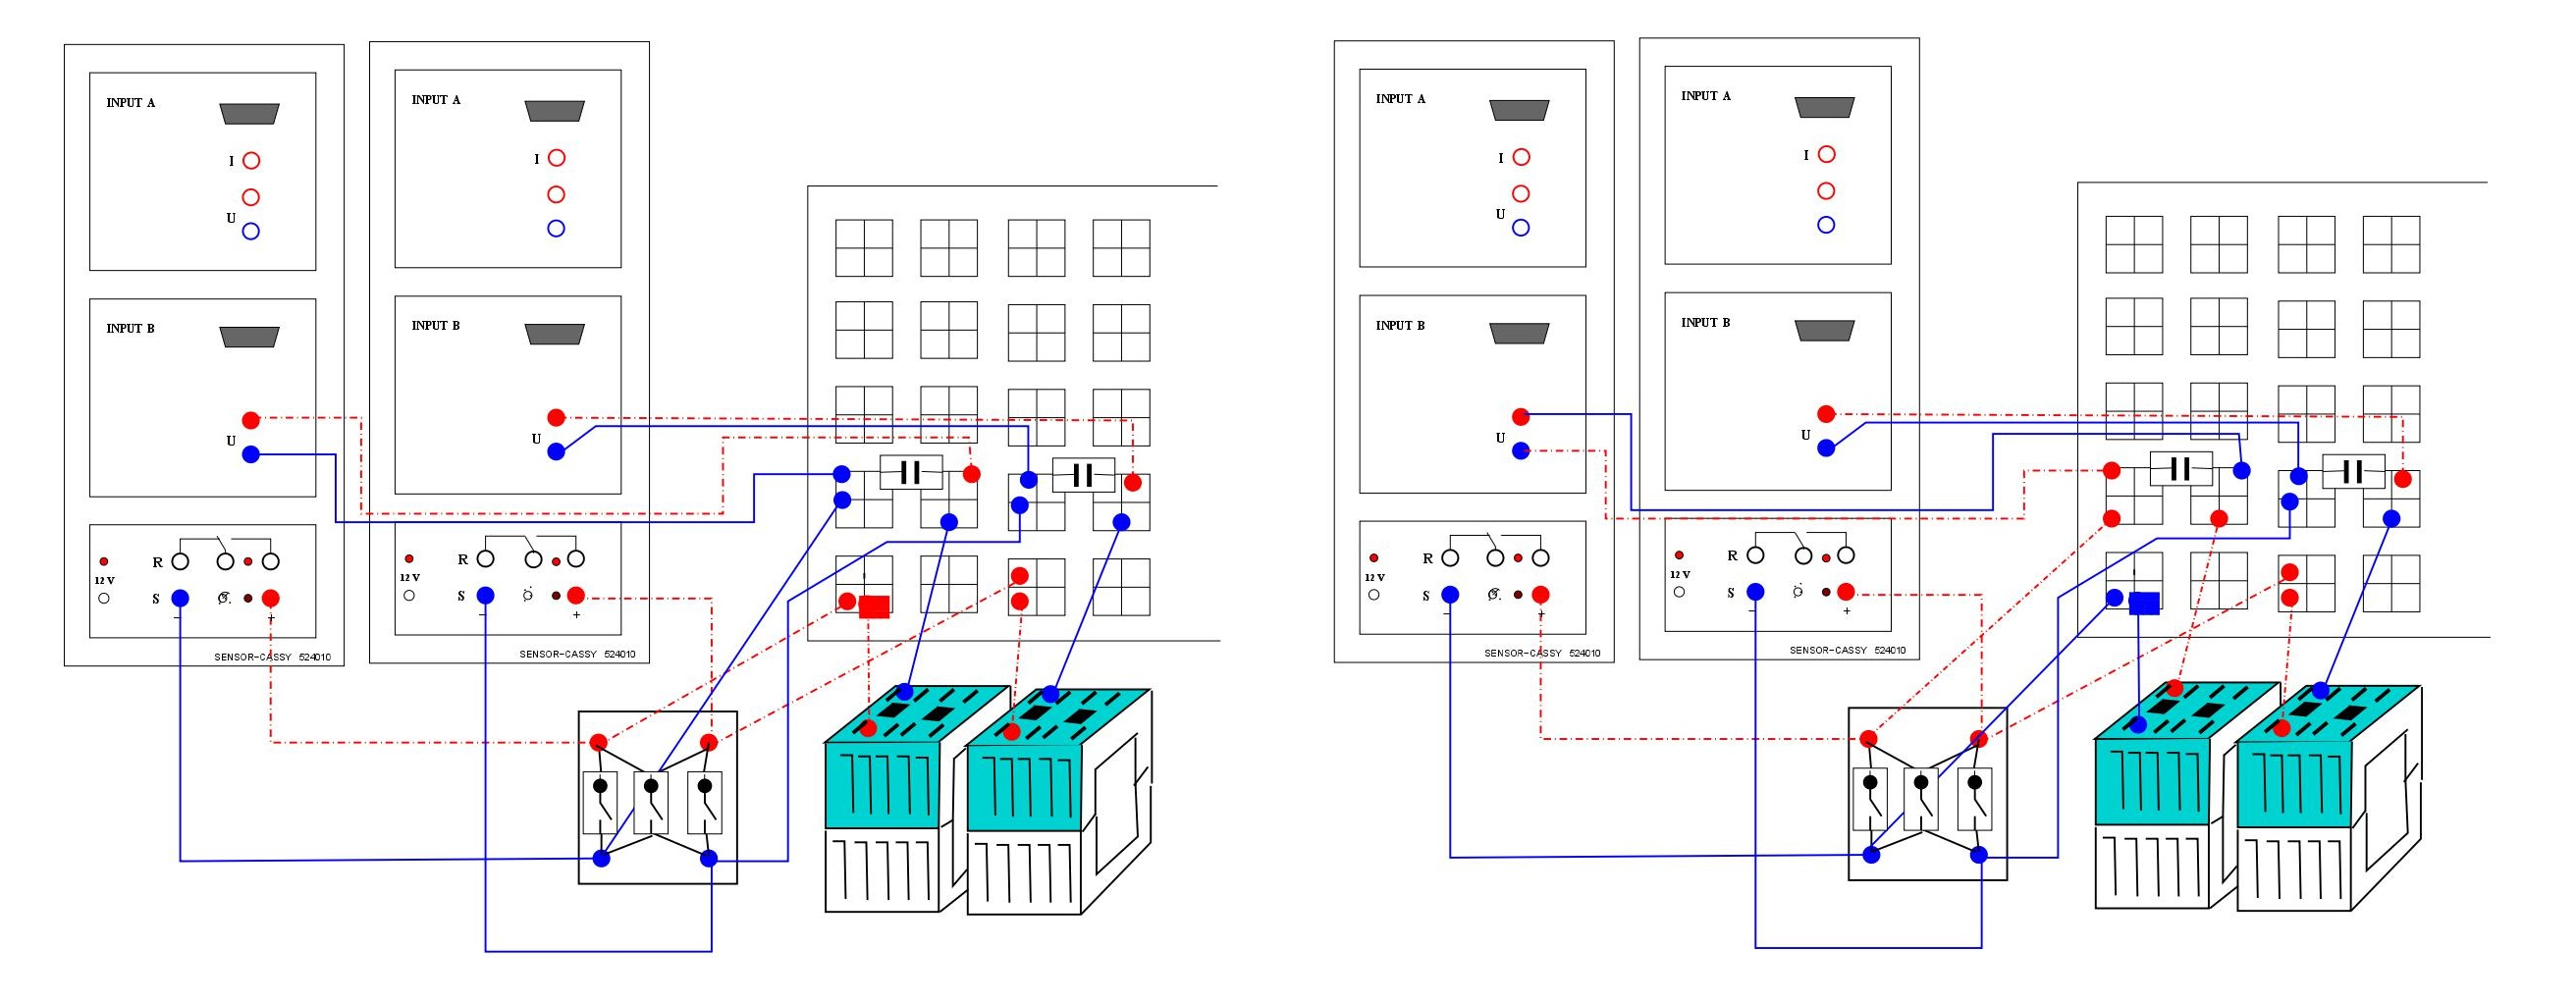
\includegraphics[width=\textwidth]{bilder/aufbau_fundamental.jpg}
\caption{Aufbau zur Anregung der Fundamentalschwingungen}
\label{abb:aufbau_fundamental}
\end{figure}

Zur Anregung der Fundamentalschwingungen werden die Aufbauten aus Abbildung \ref{abb:aufbau_fundamental} verwendet. Dabei ist links die gleichsinnige und rechts die gegensinnige Anregung zu sehen. Abweichend zur Zeichnung werden die Spannungen jeweils am Eingang A gemessen. Die Kondensatoren und Spulen sind dabei die gleichen wie bei der Aufzeichnung der Schwebung.

\subsubsection{Versuchsdurchführung}

Es werden die gleichen Messparameter wie bei der Aufzeichnung der Schwebung verwendet. Einzig die Anzahl an Messpunkten wird auf 16000 erhöht, entsprechend einer Messzeit von 160 ms. Dies dient der besseren Auflösung der Peaks im Frequenzspektrum. Die Messung wird wieder durch Betätigung des Schalters, welcher hier beide Schaltkreise gleichzeitig schaltet, gestartet. Die Spulen befinden sich ohne Eisenkern direkt aneinander.


\subsubsection{Versuchsauswertung}

Die Rohdaten zur gleichsinnigen Anregung sind in Abbildung \ref{abb:fundamental_roh} geplottet.  

\begin{figure}[H]
\centering
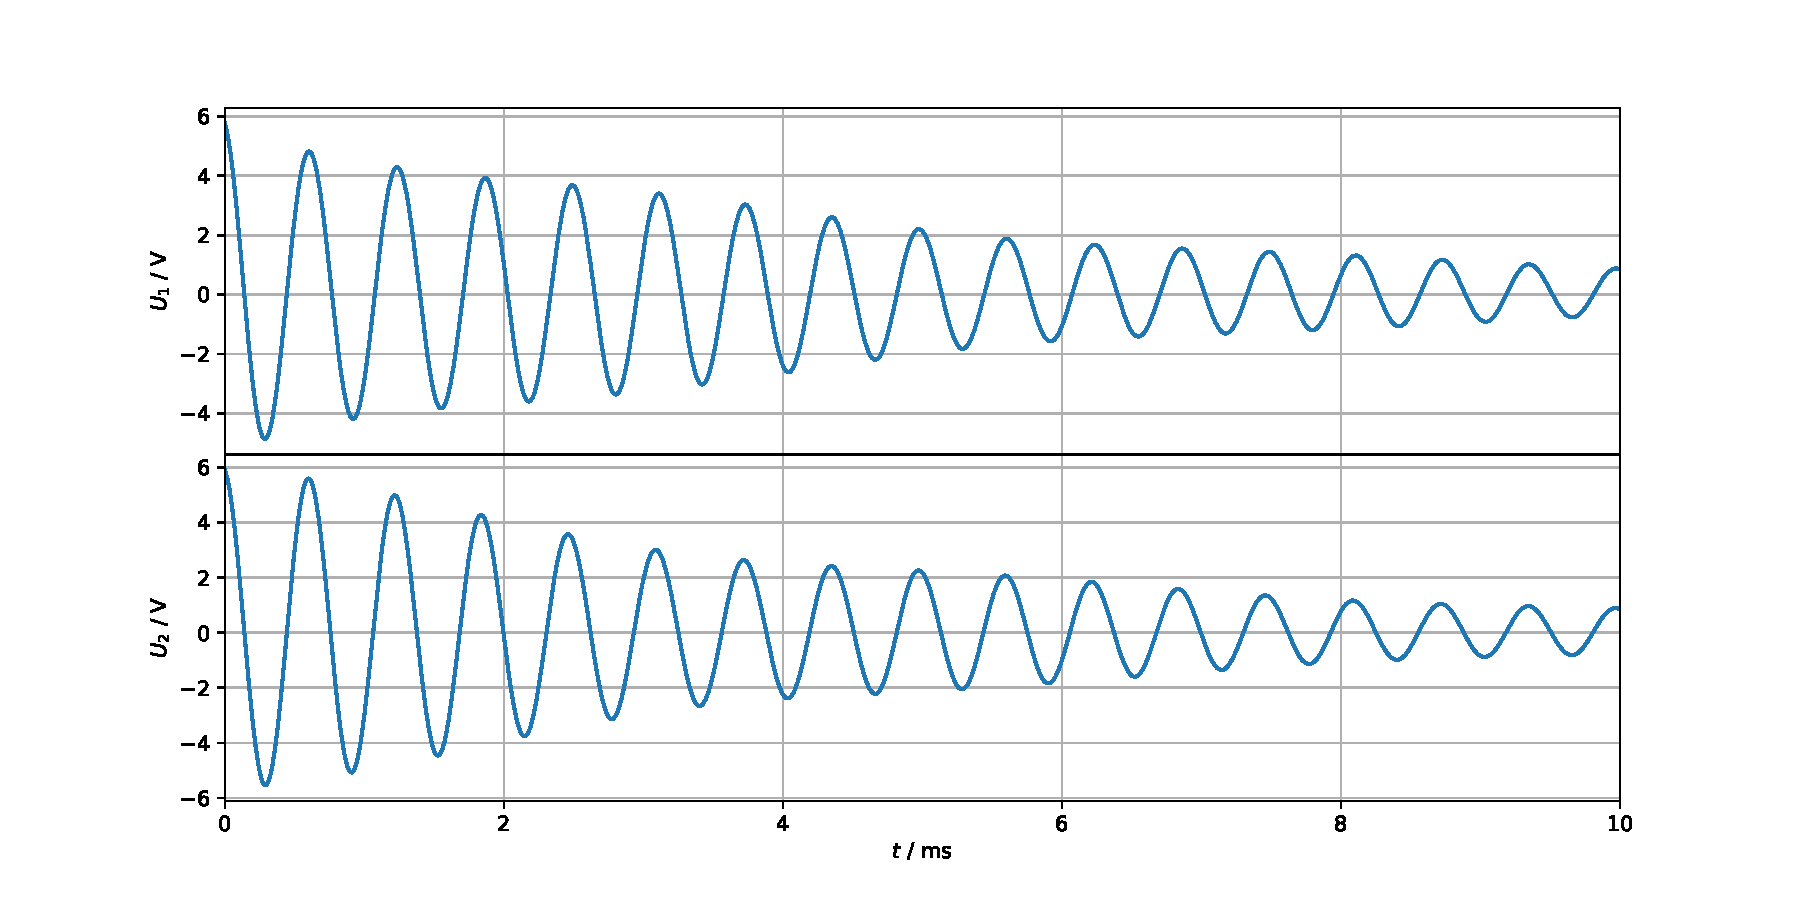
\includegraphics[width=\textwidth]{plots/fundamental_roh.pdf}
\caption{Rohdaten zur Anregung der gleichsinnigen Fundamentalschwingung}
\label{abb:fundamental_roh}
\end{figure}

Interessanter sind jedoch die Frequenzspektren der beiden Anregungen. Diese befinden sich in Abbildung \ref{abb:FFT_fundamental}.

\begin{figure}[H]
\centering
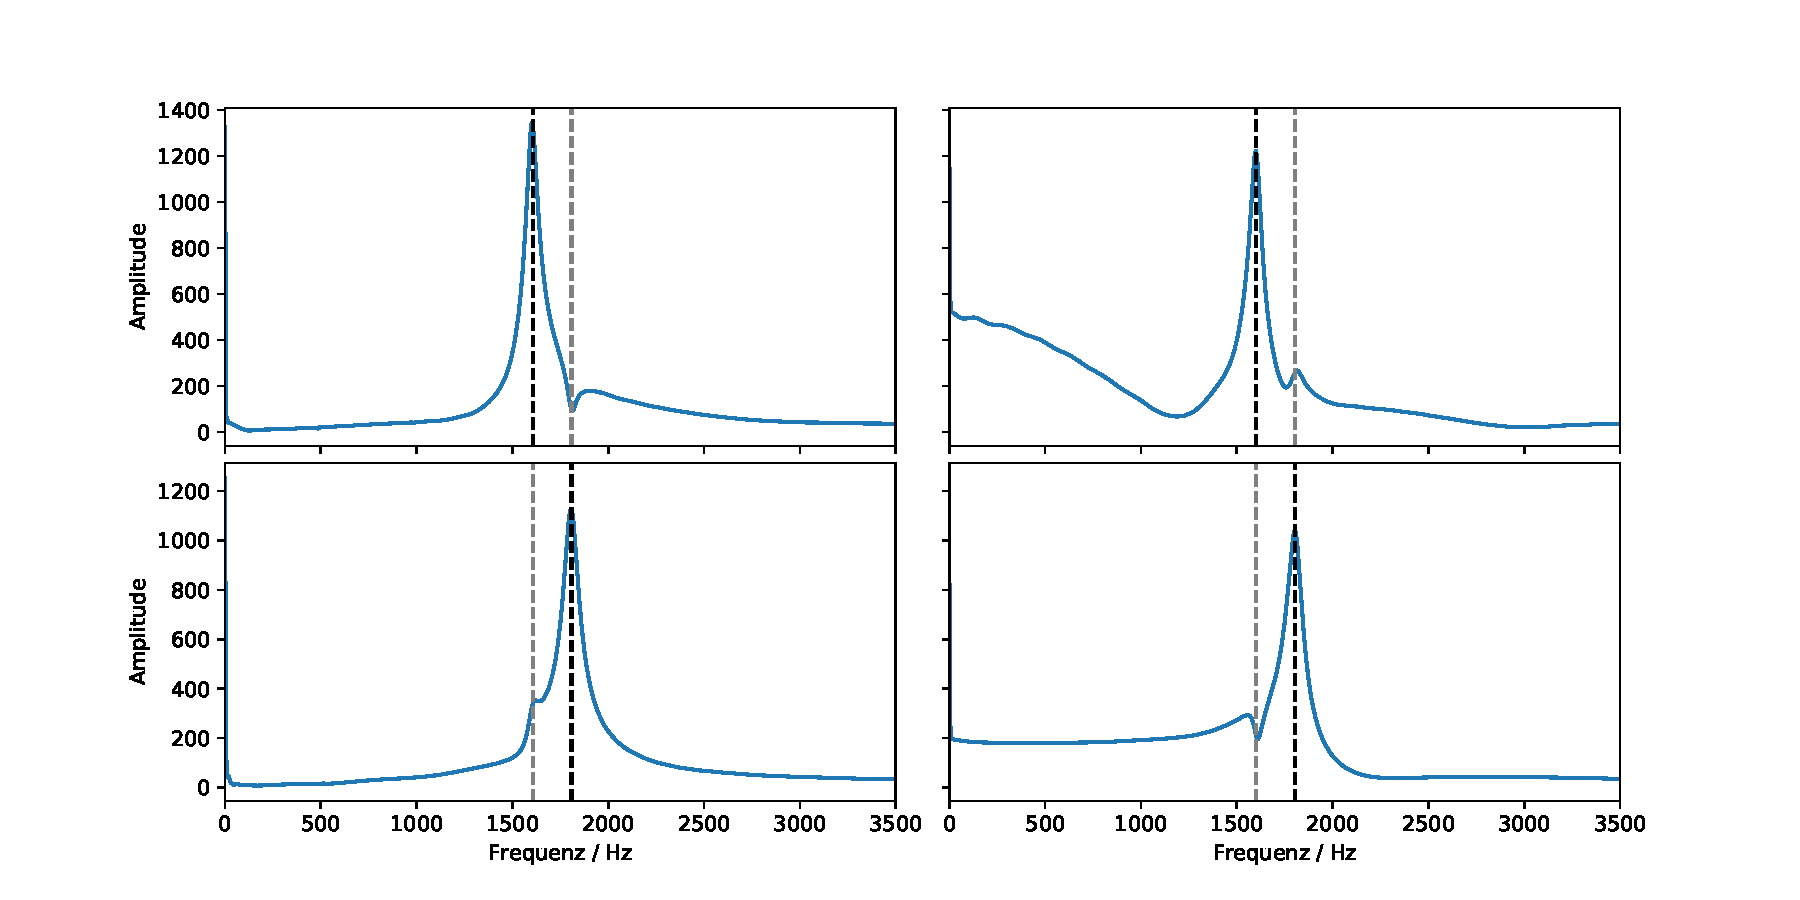
\includegraphics[width=\textwidth]{plots/fundamental_fft.pdf}
\caption{Frequenzspektren der Fundamentalschwingungen}
\label{abb:FFT_fundamental}
\end{figure}

Dabei sind oben die gleichsinnigen und unten die gegensinnigen Anregungen zu sehen. Zudem ist jeweils links der erste und rechts der zweite Schwingkreis. Die Frequenzen stimmen in etwa mit den Frequenzen aus Schwebung 1 überein. Die Abweichungen können vor allem durch der veränderten Aufbau bedingt sein.

\subsubsection{Fazit}

Es war äußerst schwierig die Fundamentalschwingungen zu treffen. Durch leicht unterschiedliche Bauteile und die schwierige gleichzeitige Schaltung der beiden Schwingkreise sind die erhaltenen Schwingungen eher Zufallsprodukte gewesen. Man sieht im Frequenzspektrum zudem, dass die zweite Fundamentalschwingung auch leicht angeregt wird.



\newpage
\appendix
\section{LCR-Schwingfall: Regressionen der übrigen Widerstände}\label{app:reg}
\begin{figure}[H]
\centering
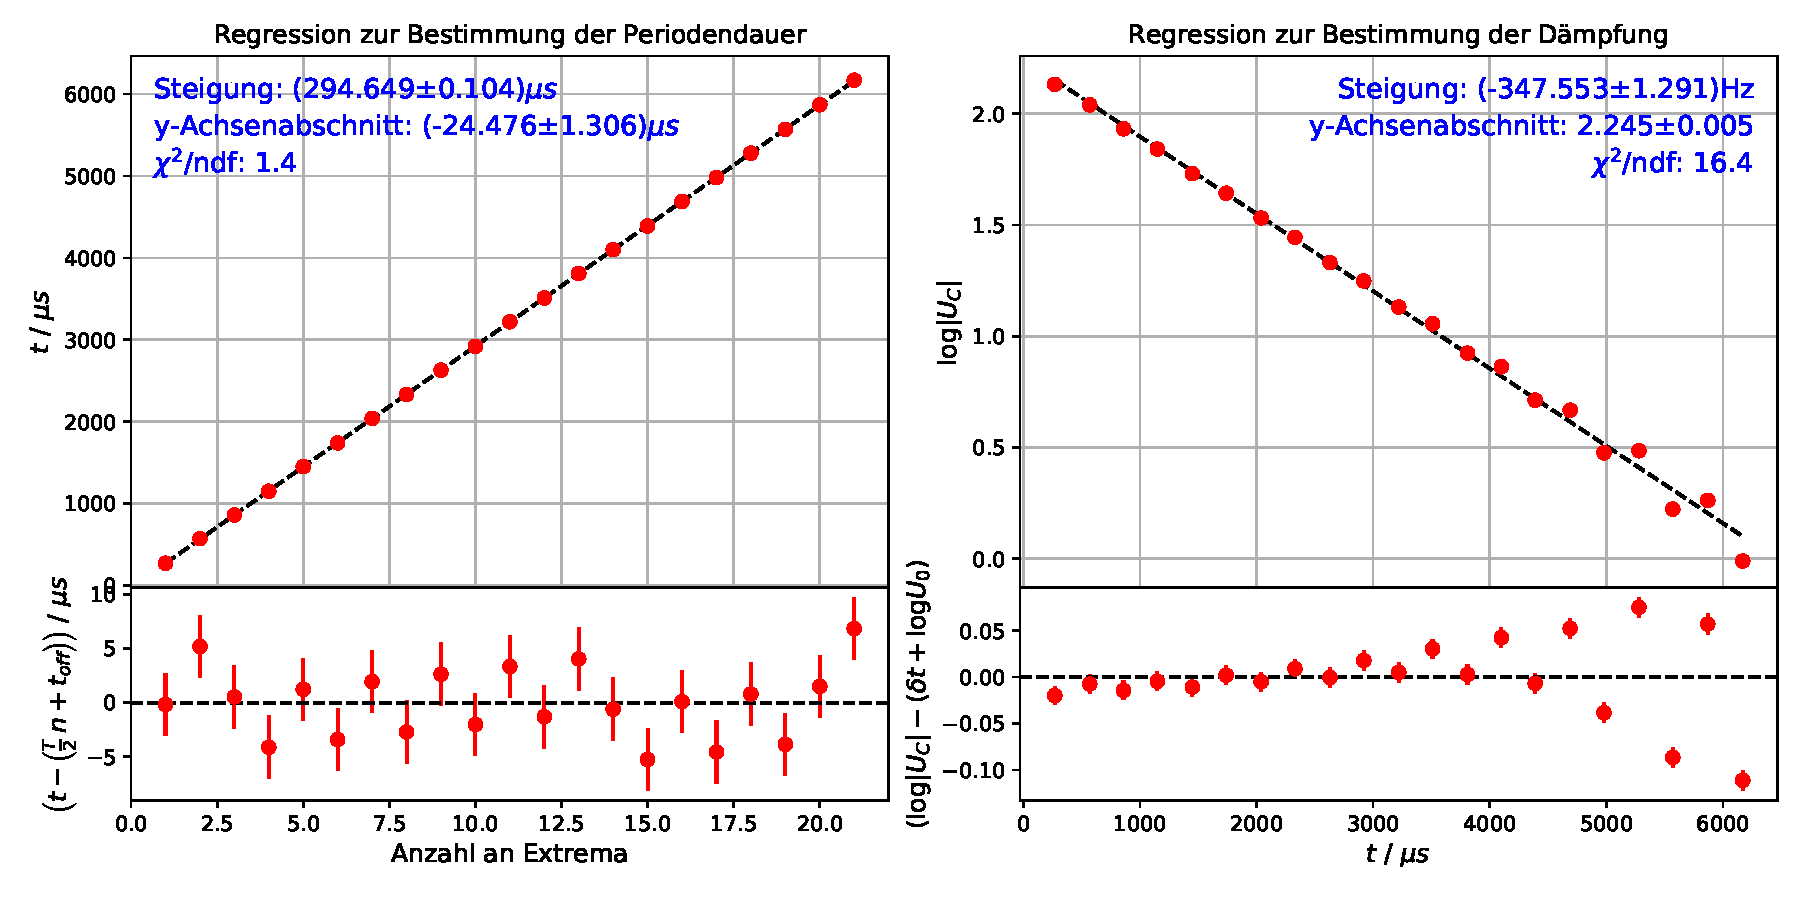
\includegraphics[width=\textwidth]{plots/reg_schwingung1.pdf}
\caption{Regressionen für den $1\Omega$ Widerstand zur Bestimmung von $\frac{T}{2}$ und $\delta$}
\end{figure}
\begin{figure}[H]
\centering
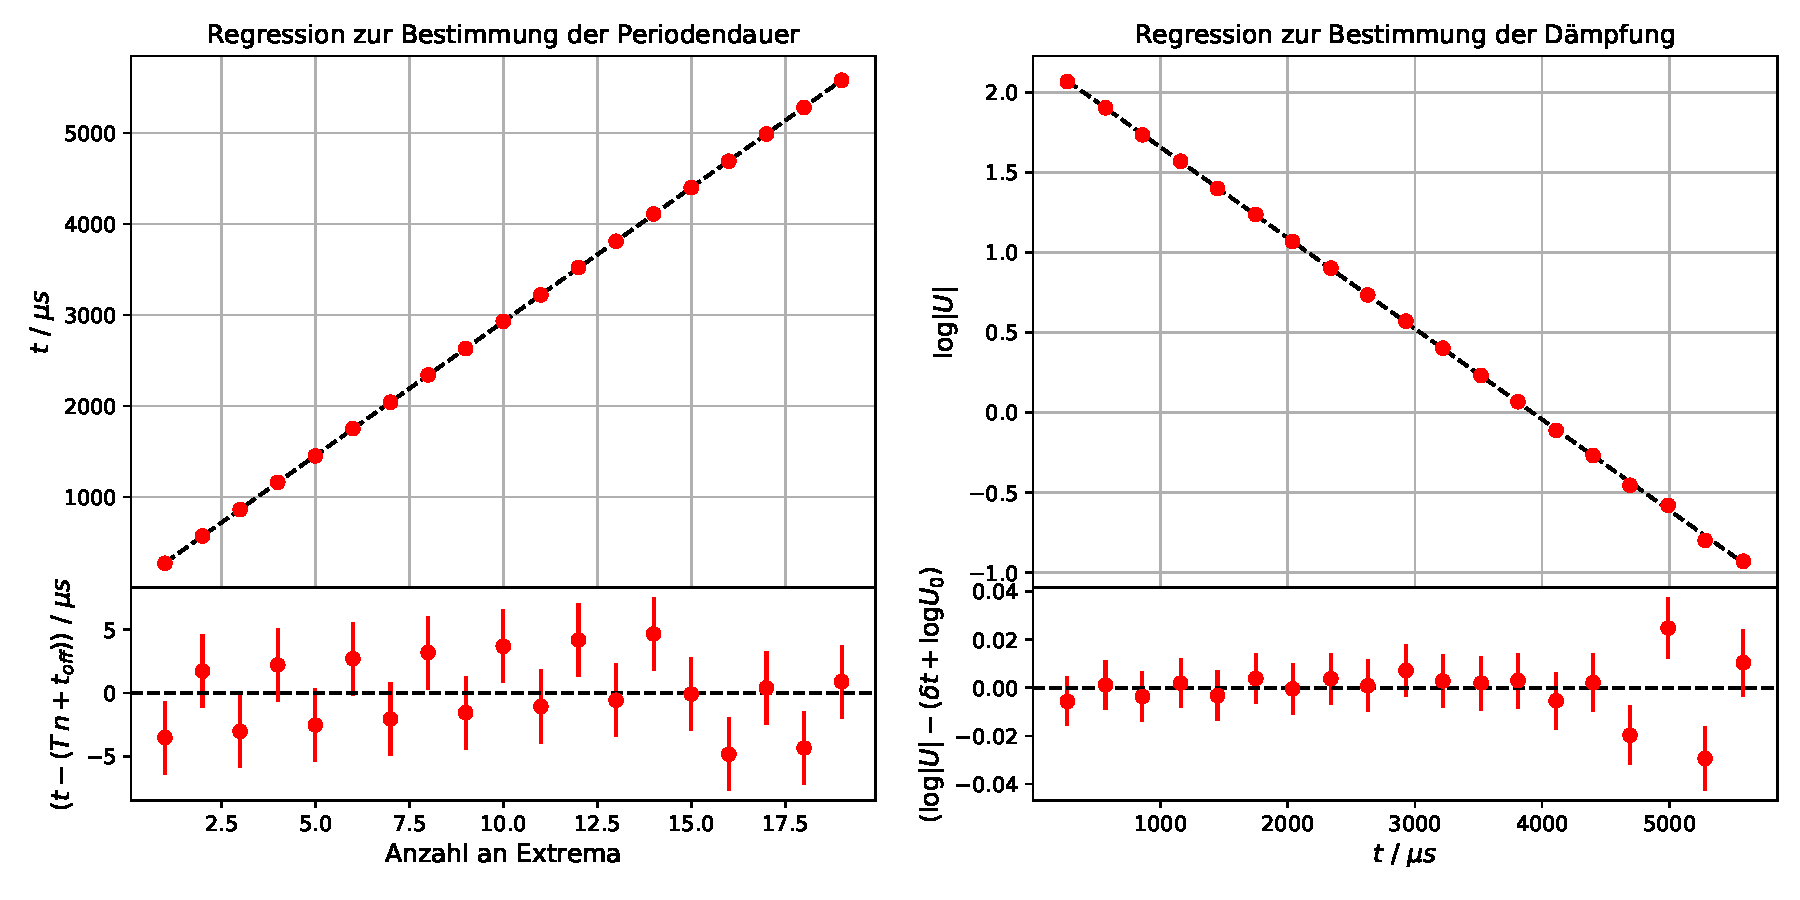
\includegraphics[width=\textwidth]{plots/reg_schwingung2.pdf}
\caption{Regressionen für den $5.1\Omega$ Widerstand zur Bestimmung von $\frac{T}{2}$ und $\delta$}
\end{figure}
\begin{figure}[H]
\centering
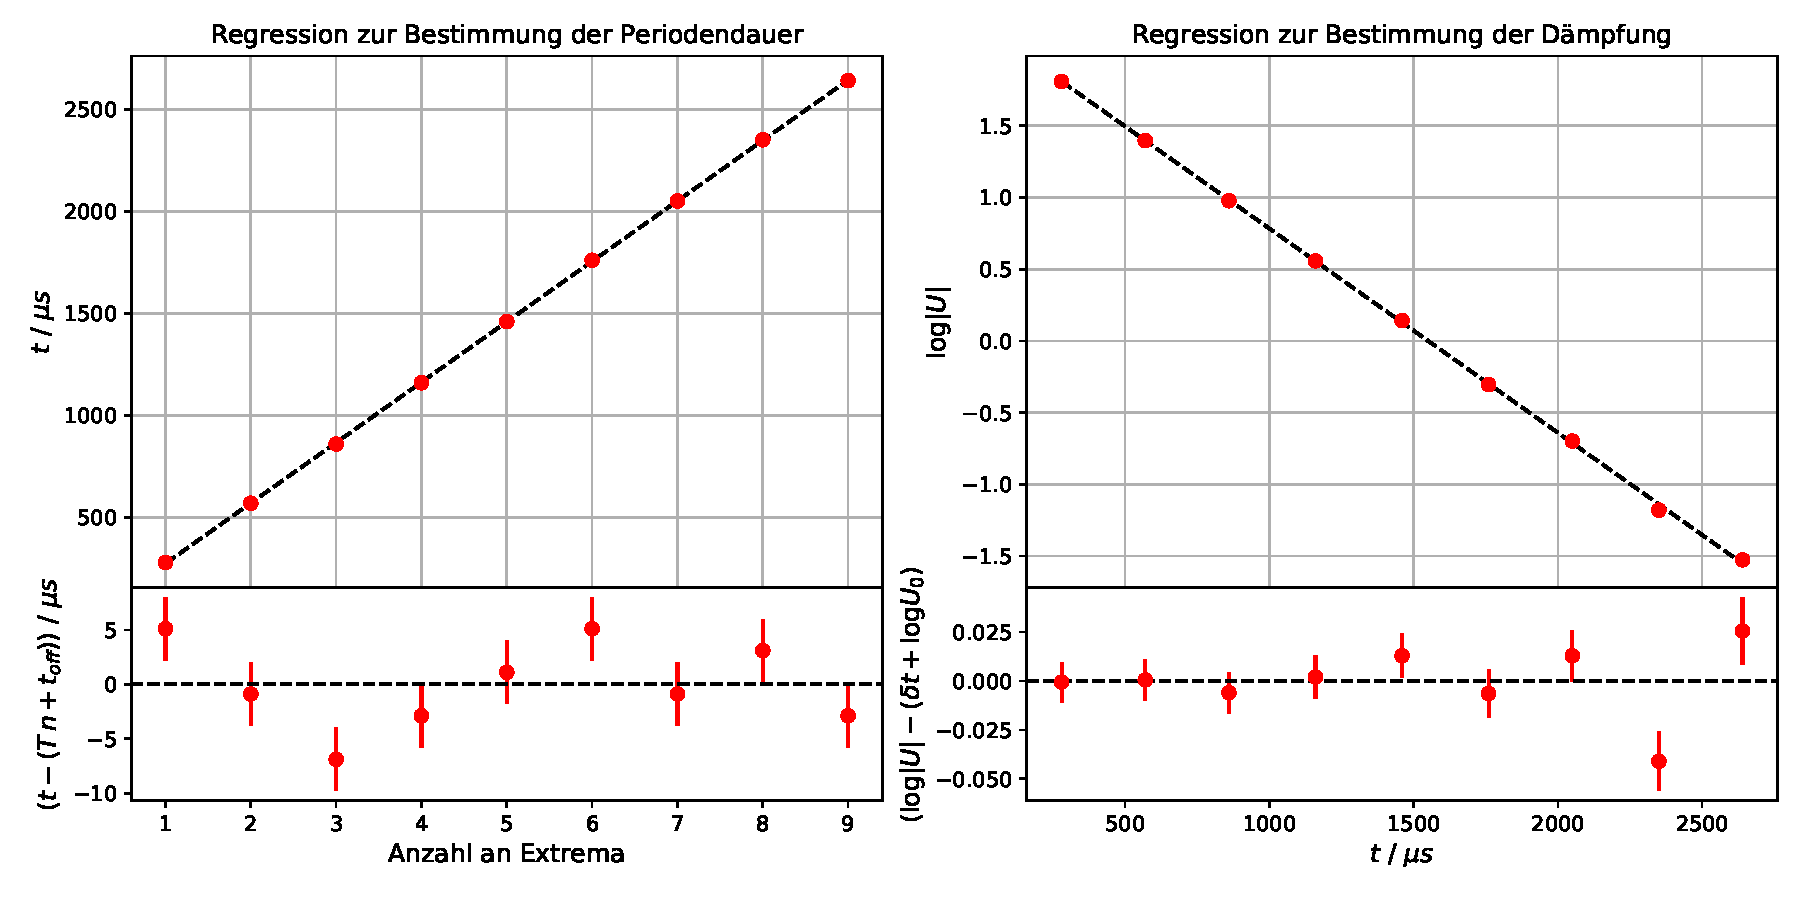
\includegraphics[width=\textwidth]{plots/reg_schwingung4.pdf}
\caption{Regressionen für den $20\Omega$ Widerstand zur Bestimmung von $\frac{T}{2}$ und $\delta$}
\end{figure}
\begin{figure}[H]
\centering
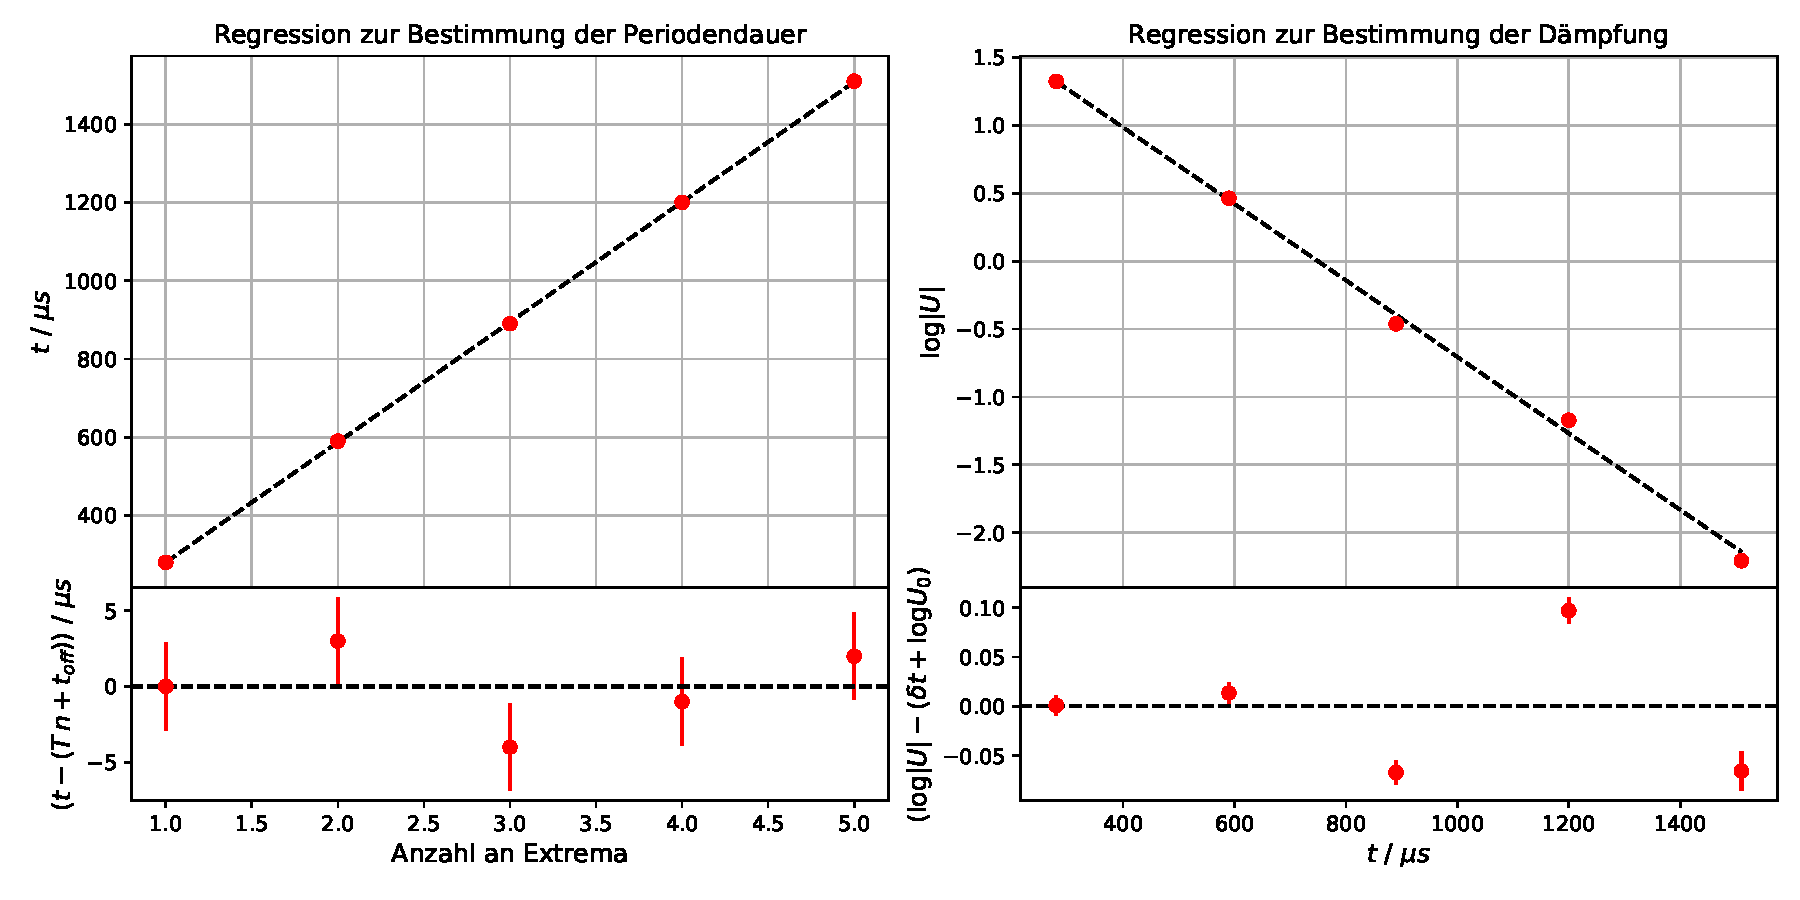
\includegraphics[width=\textwidth]{plots/reg_schwingung5.pdf}
\caption{Regressionen für den $47\Omega$ Widerstand zur Bestimmung von $\frac{T}{2}$ und $\delta$}
\end{figure}

\section{LCR-Schwingfall: FFT der übrigen Widerstände}\label{app:fft}
\begin{figure}[H]
\centering
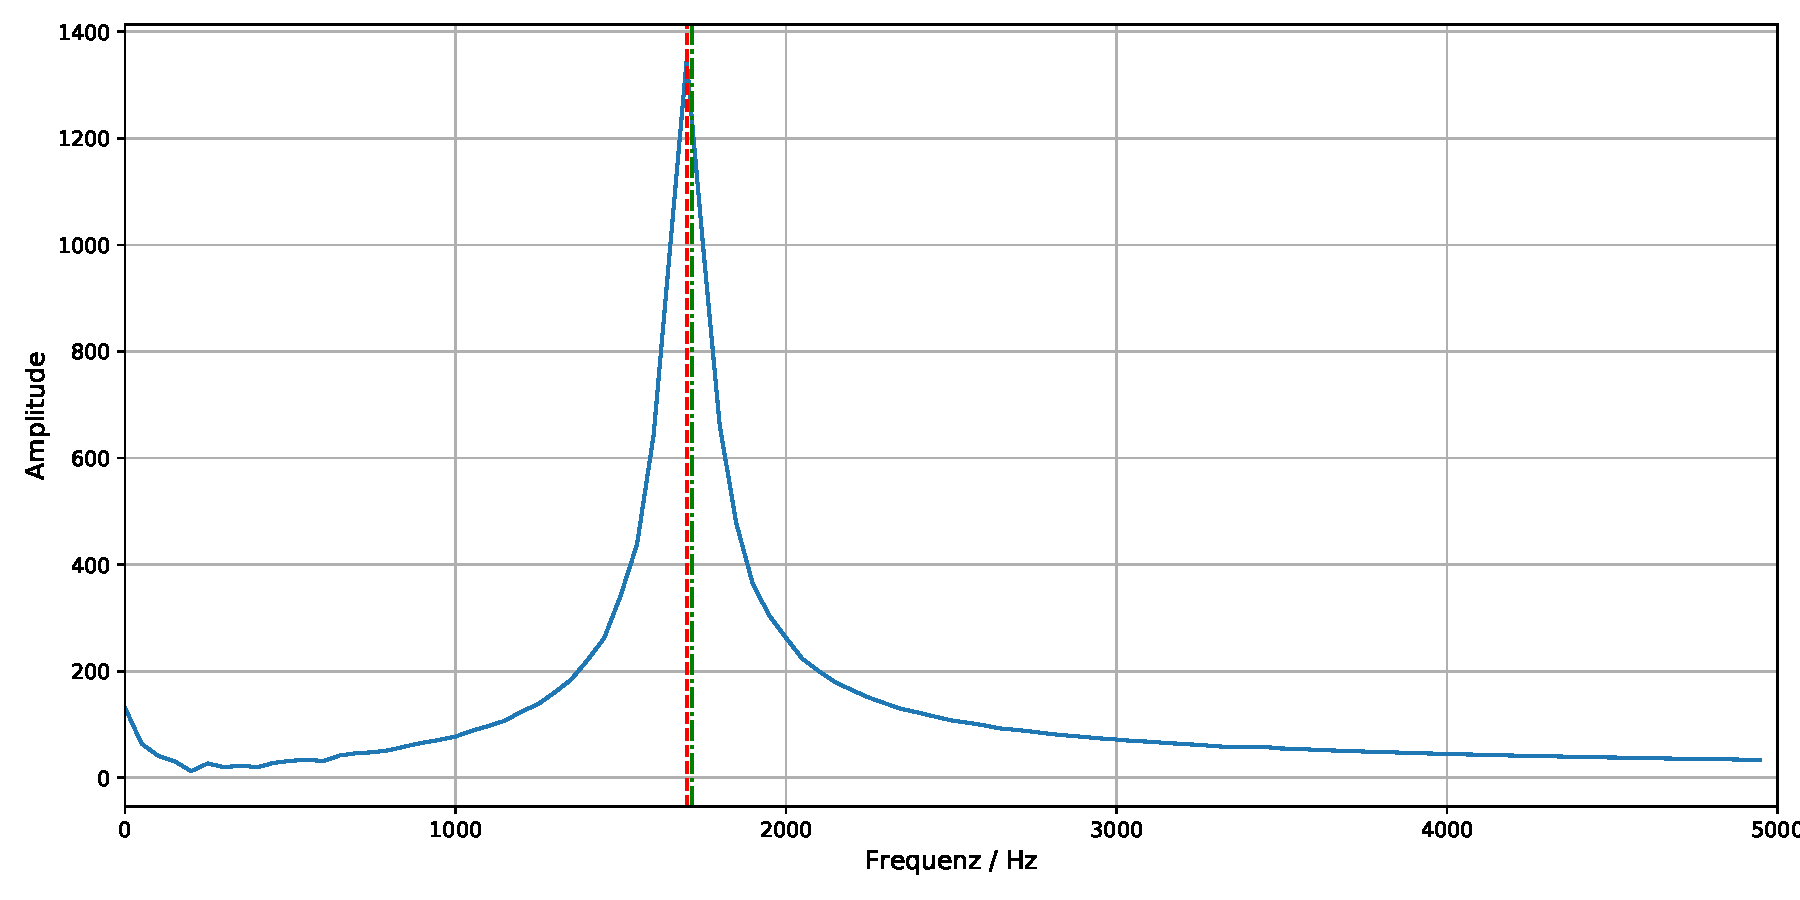
\includegraphics[width=\textwidth]{plots/fft/fft_schwingung1_1.pdf}
\caption{Mittels FFT berechnetes Spektrum für die erste Messung des $1\Omega$ Widerstands. Die rote Linie zeigt das Argument-Maximum an. Die grüne Linie Hingegen den Peak-Schwerpunkt.}
\end{figure}
\begin{figure}[H]
\centering
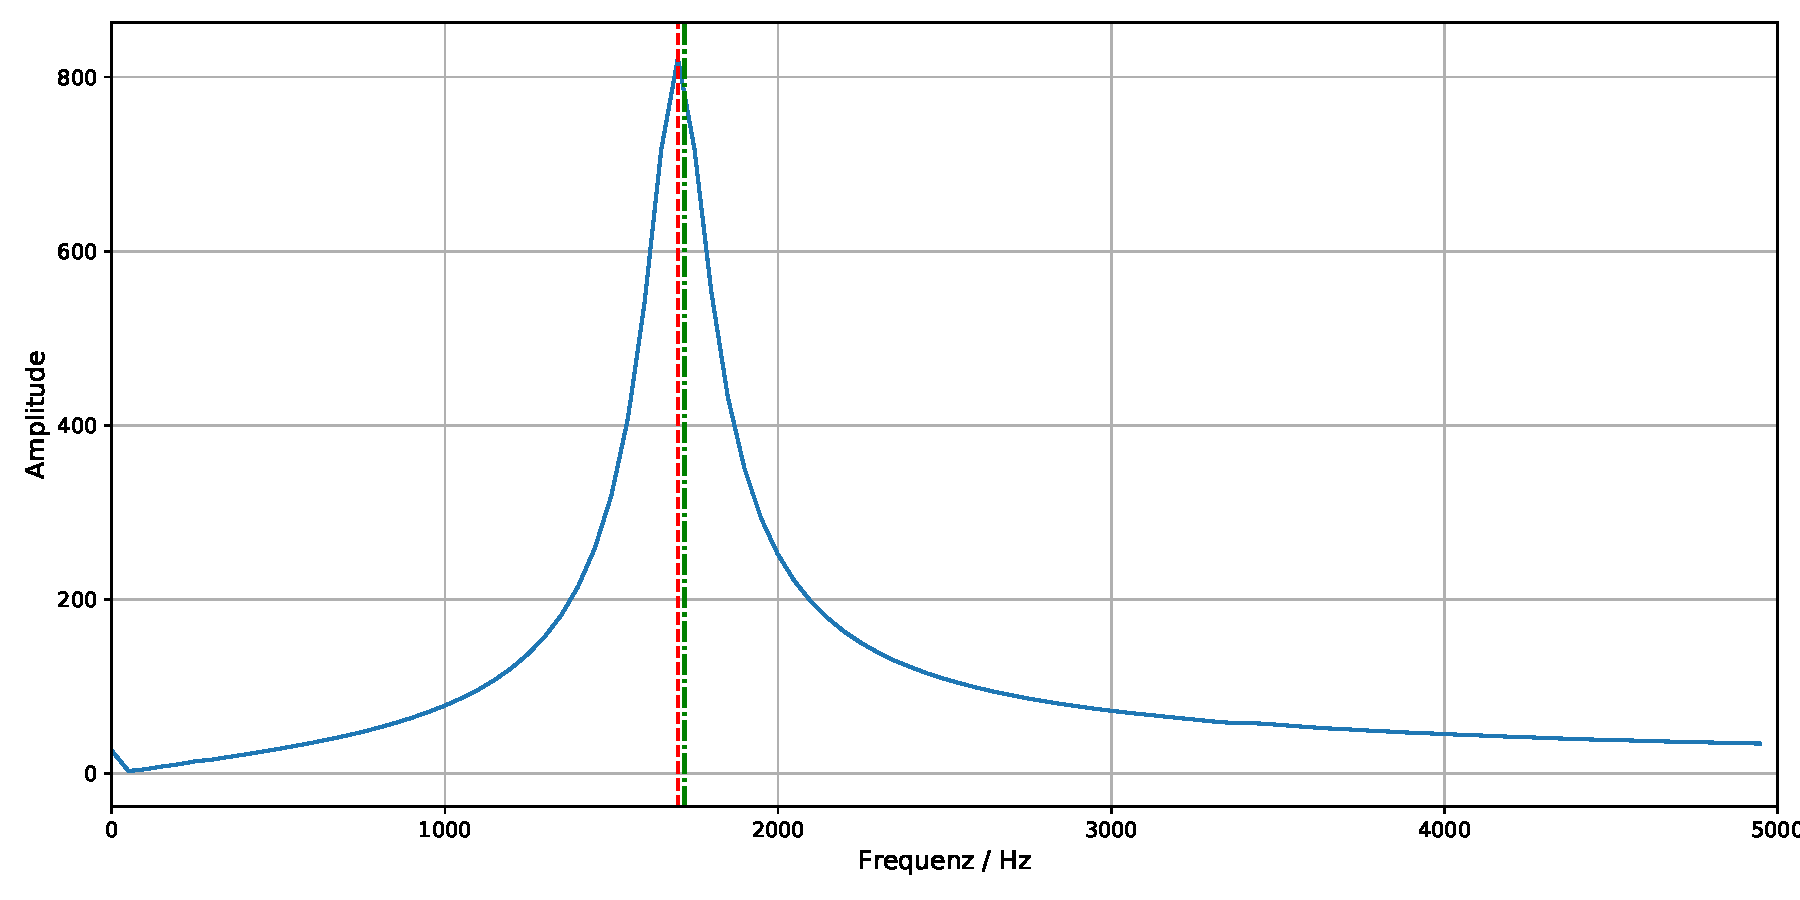
\includegraphics[width=\textwidth]{plots/fft/fft_schwingung2_1.pdf}
\caption{Mittels FFT berechnetes Spektrum für die erste Messung des $5.1\Omega$ Widerstands. Die rote Linie zeigt das Argument-Maximum an. Die grüne Linie Hingegen den Peak-Schwerpunkt.}
\end{figure}
\begin{figure}[H]
\centering
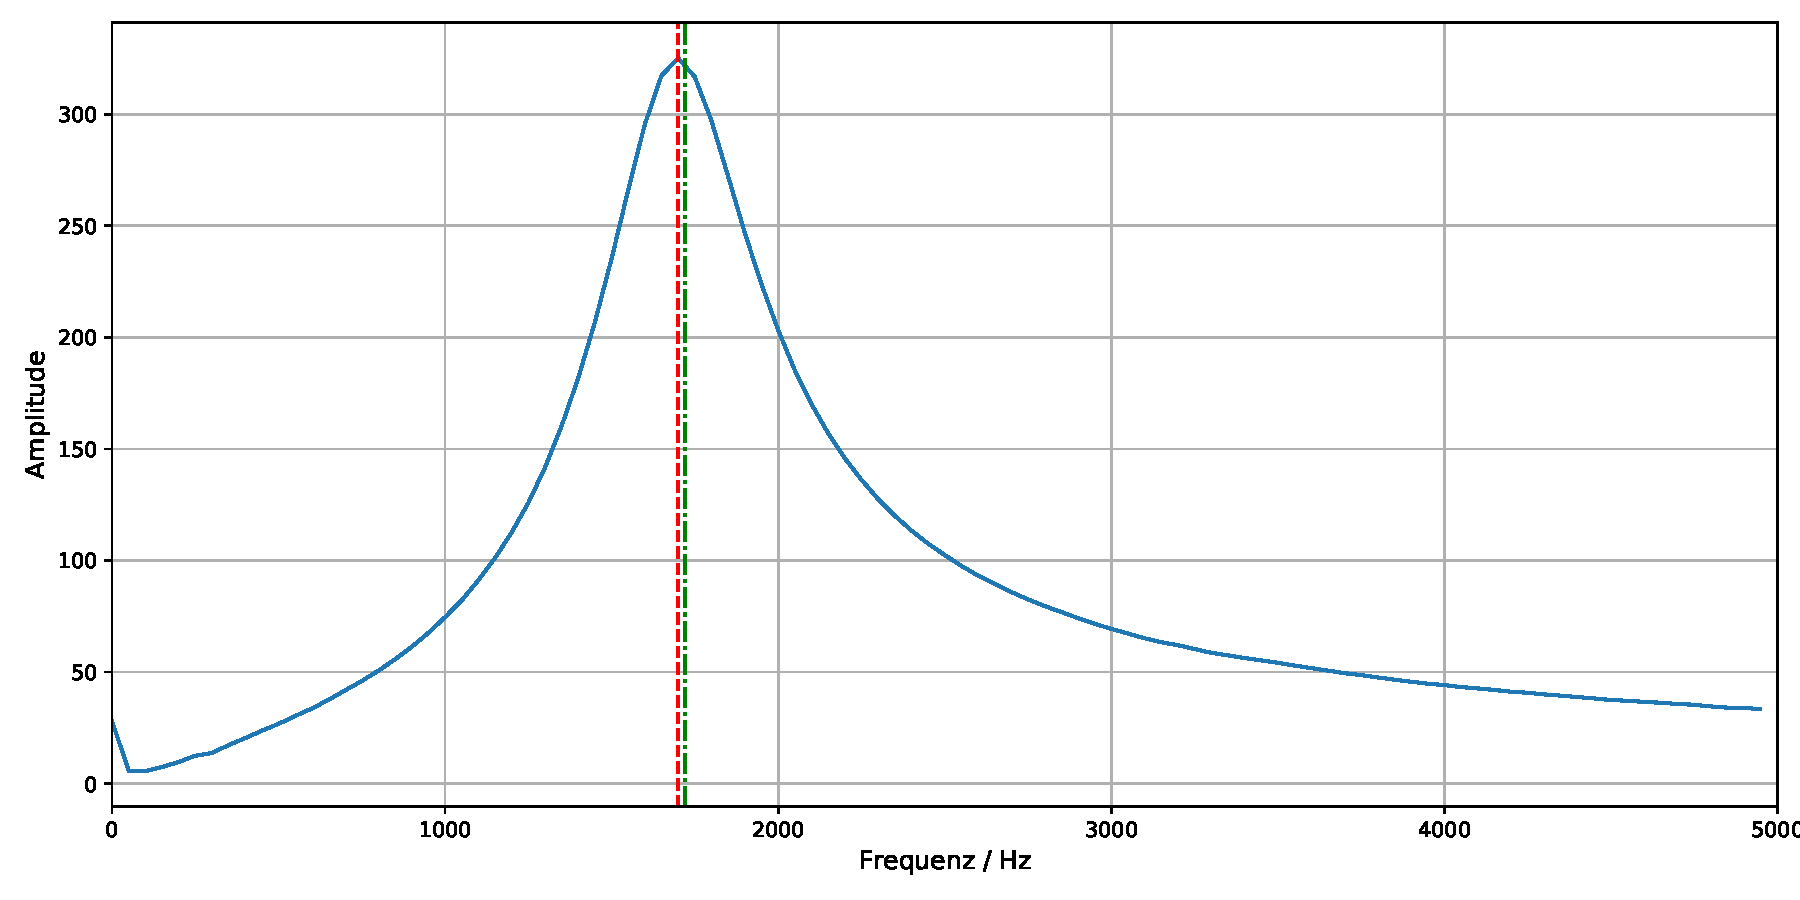
\includegraphics[width=\textwidth]{plots/fft/fft_schwingung4_1.pdf}
\caption{Mittels FFT berechnetes Spektrum für die erste Messung des $20\Omega$ Widerstands. Die rote Linie zeigt das Argument-Maximum an. Die grüne Linie Hingegen den Peak-Schwerpunkt.}
\end{figure}
\begin{figure}[H]
\centering
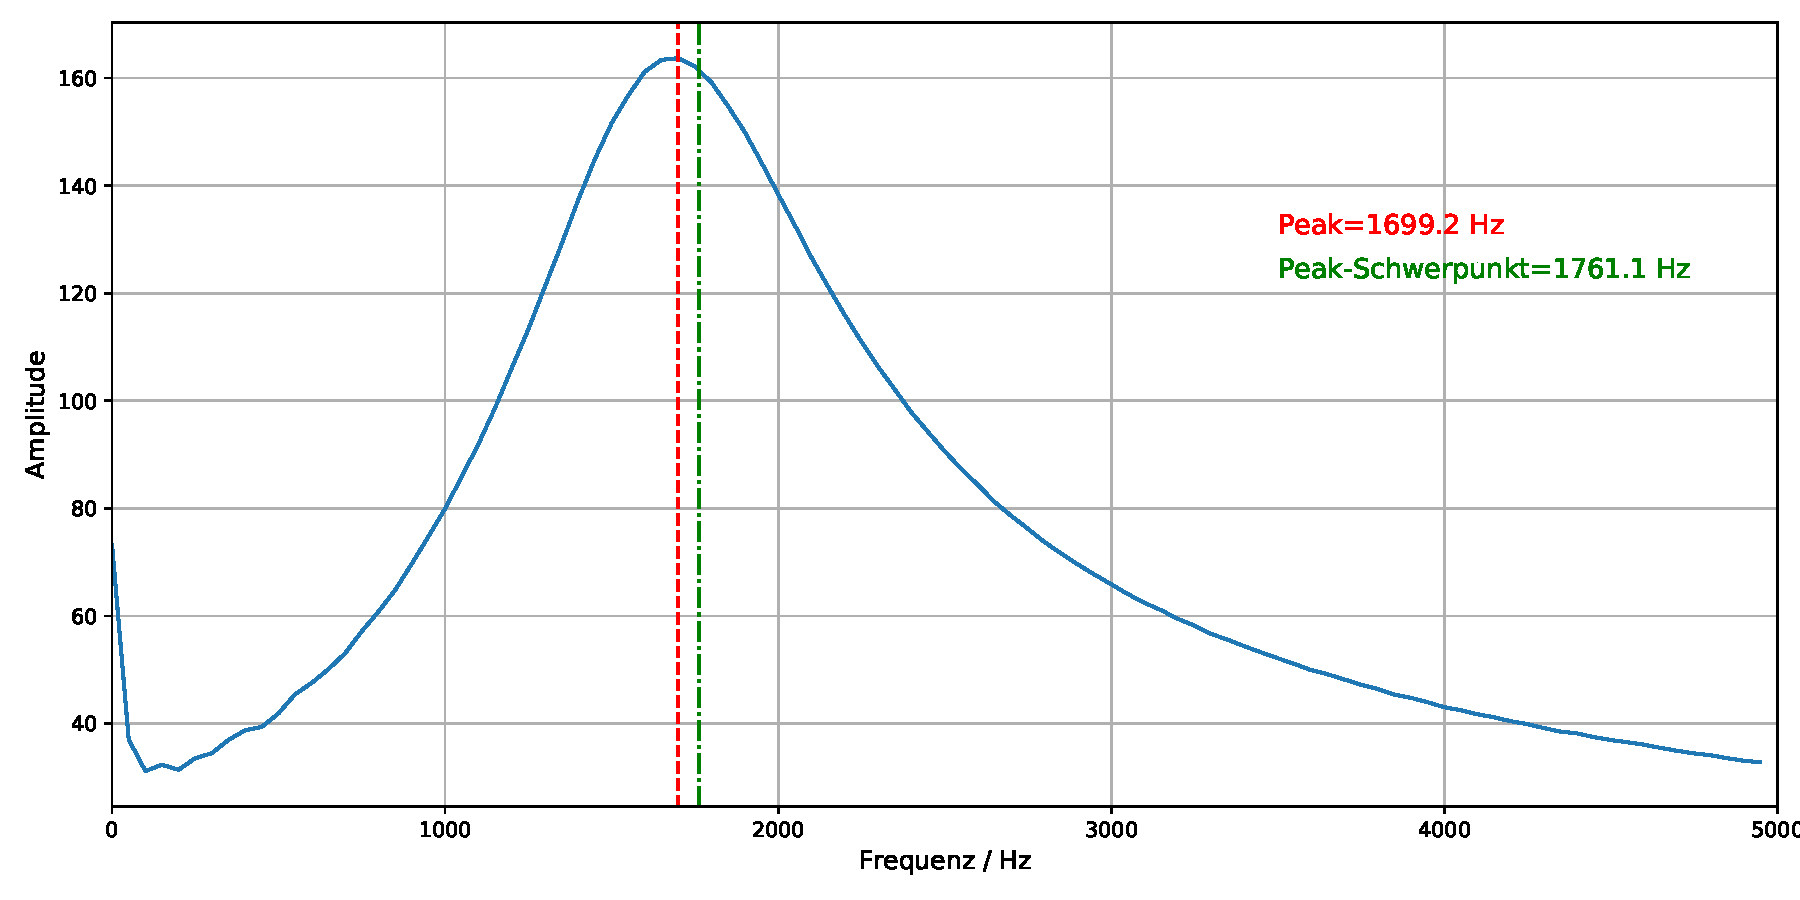
\includegraphics[width=\textwidth]{plots/fft/fft_schwingung5_1.pdf}
\caption{Mittels FFT berechnetes Spektrum für die erste Messung des $47\Omega$ Widerstands. Die rote Linie zeigt das Argument-Maximum an. Die grüne Linie Hingegen den Peak-Schwerpunkt.}
\end{figure}
\begin{figure}[H]
\centering
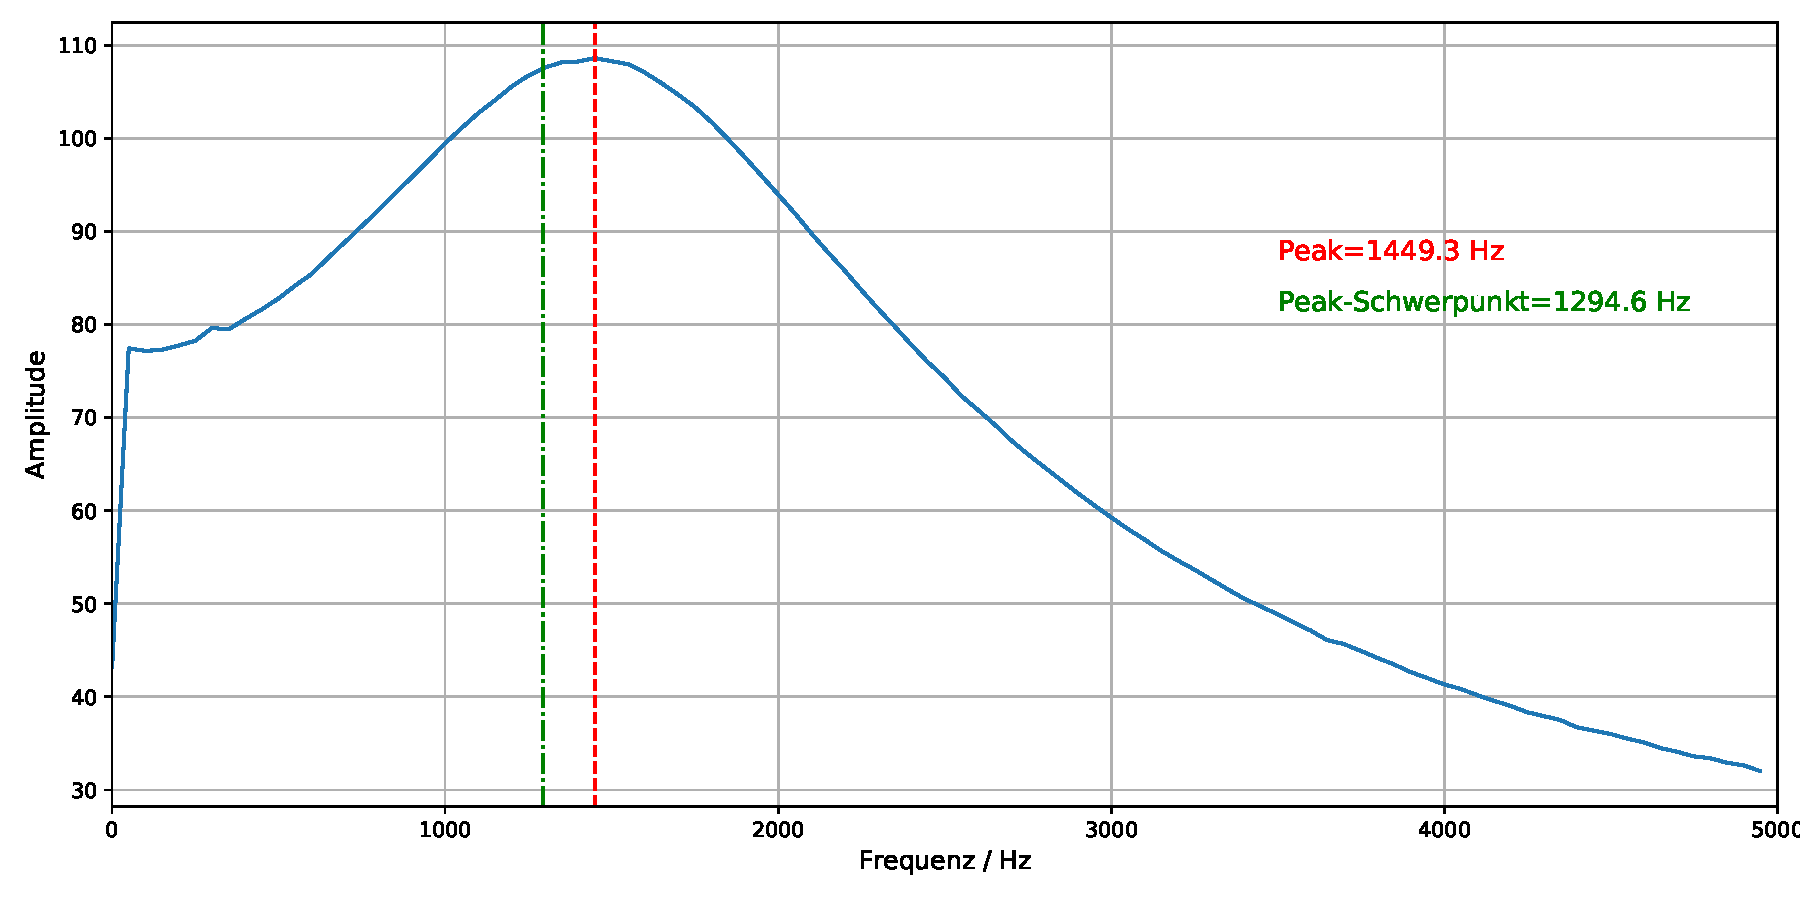
\includegraphics[width=\textwidth]{plots/fft/fft_schwingung6_1.pdf}
\caption{Mittels FFT berechnetes Spektrum für die erste Messung des $100\Omega$ Widerstands. Die rote Linie zeigt das Argument-Maximum an. Die grüne Linie Hingegen den Peak-Schwerpunkt.}
\end{figure}

\section{LCR-Schwingfall: Exp-Einhüllende der übrigen Widerstände}\label{app:expein}
\begin{figure}[h]
\centering
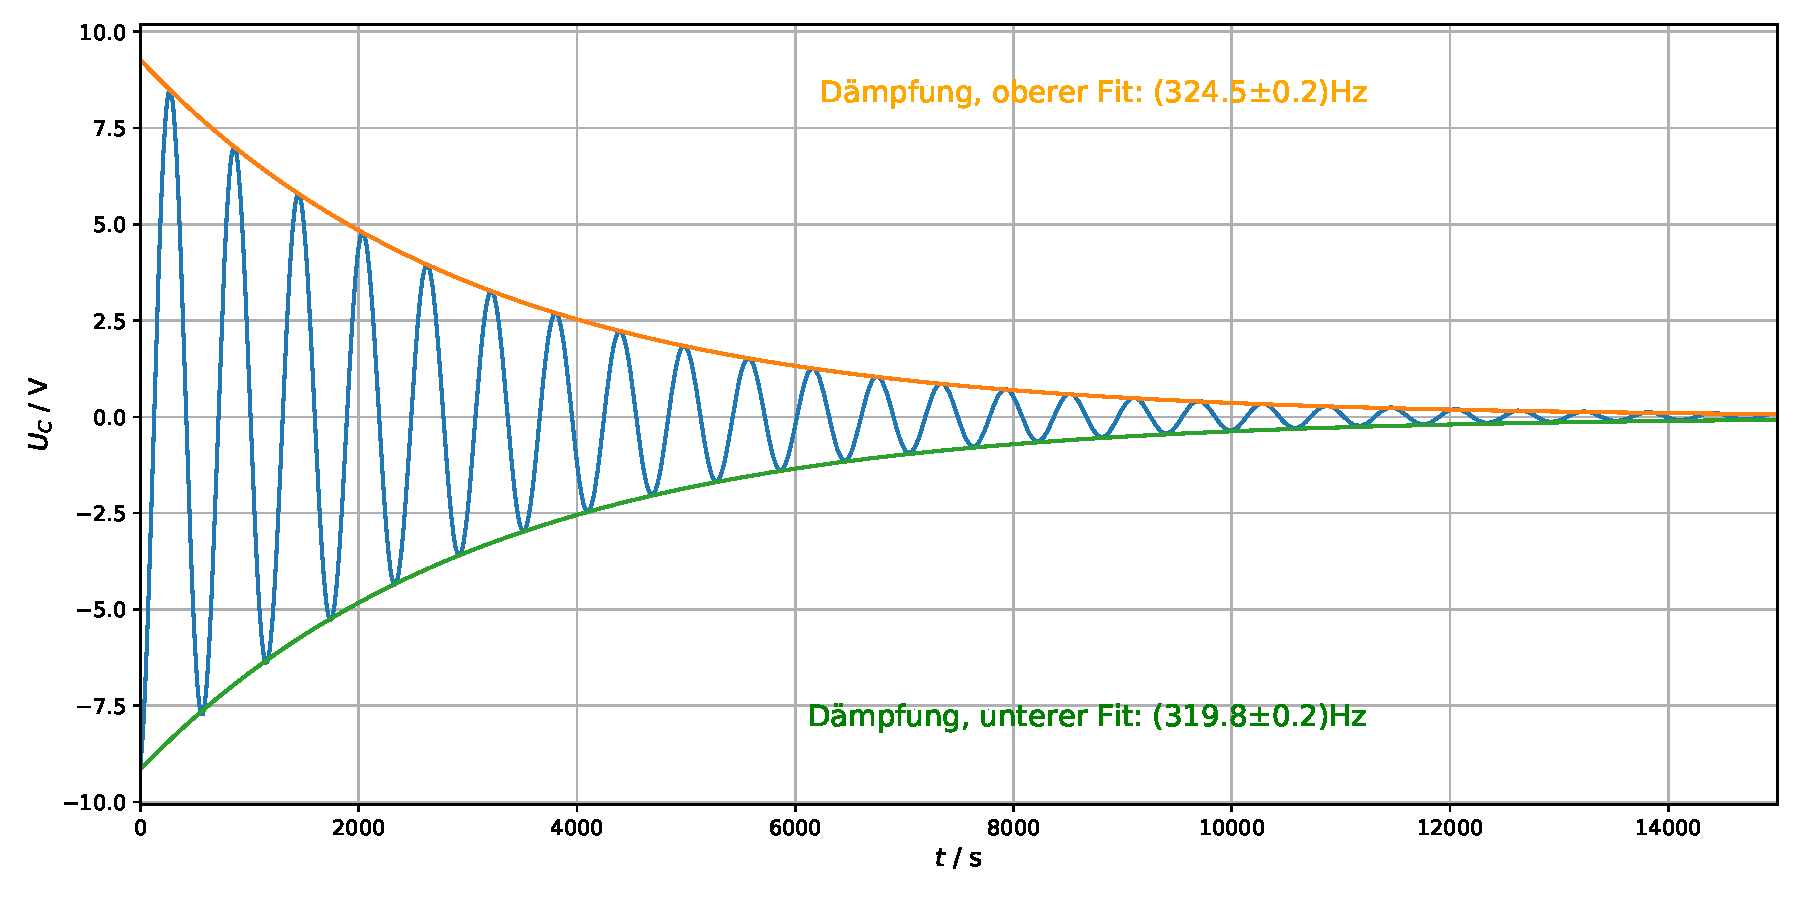
\includegraphics[width=\textwidth]{plots/einhuellend/exp_einhuellend1_2.pdf}
\caption{Mittels Python berechnete exponentiell Einhüllende für die zweite Messung des $1\Omega$ Widerstands.}
\end{figure}
\begin{figure}[h]
\centering
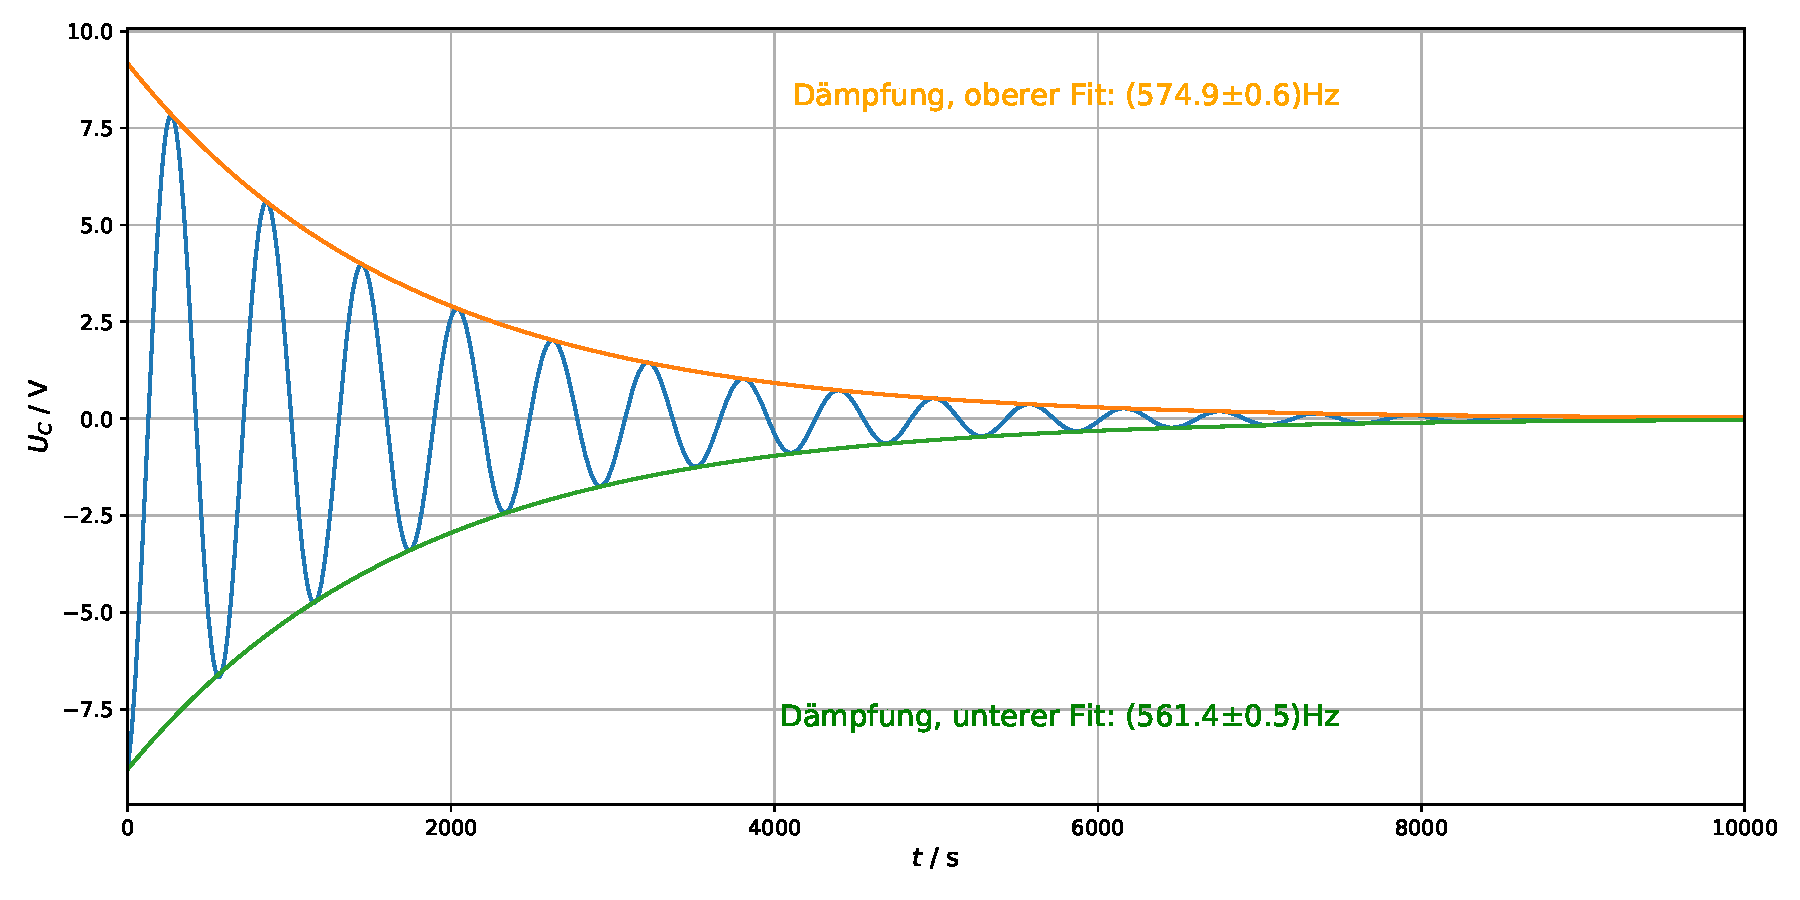
\includegraphics[width=\textwidth]{plots/einhuellend/exp_einhuellend2_2.pdf}
\caption{Mittels Python berechnete exponentiell Einhüllende für die zweite Messung des $5.1\Omega$ Widerstands.}
\end{figure}
\begin{figure}[h]
\centering
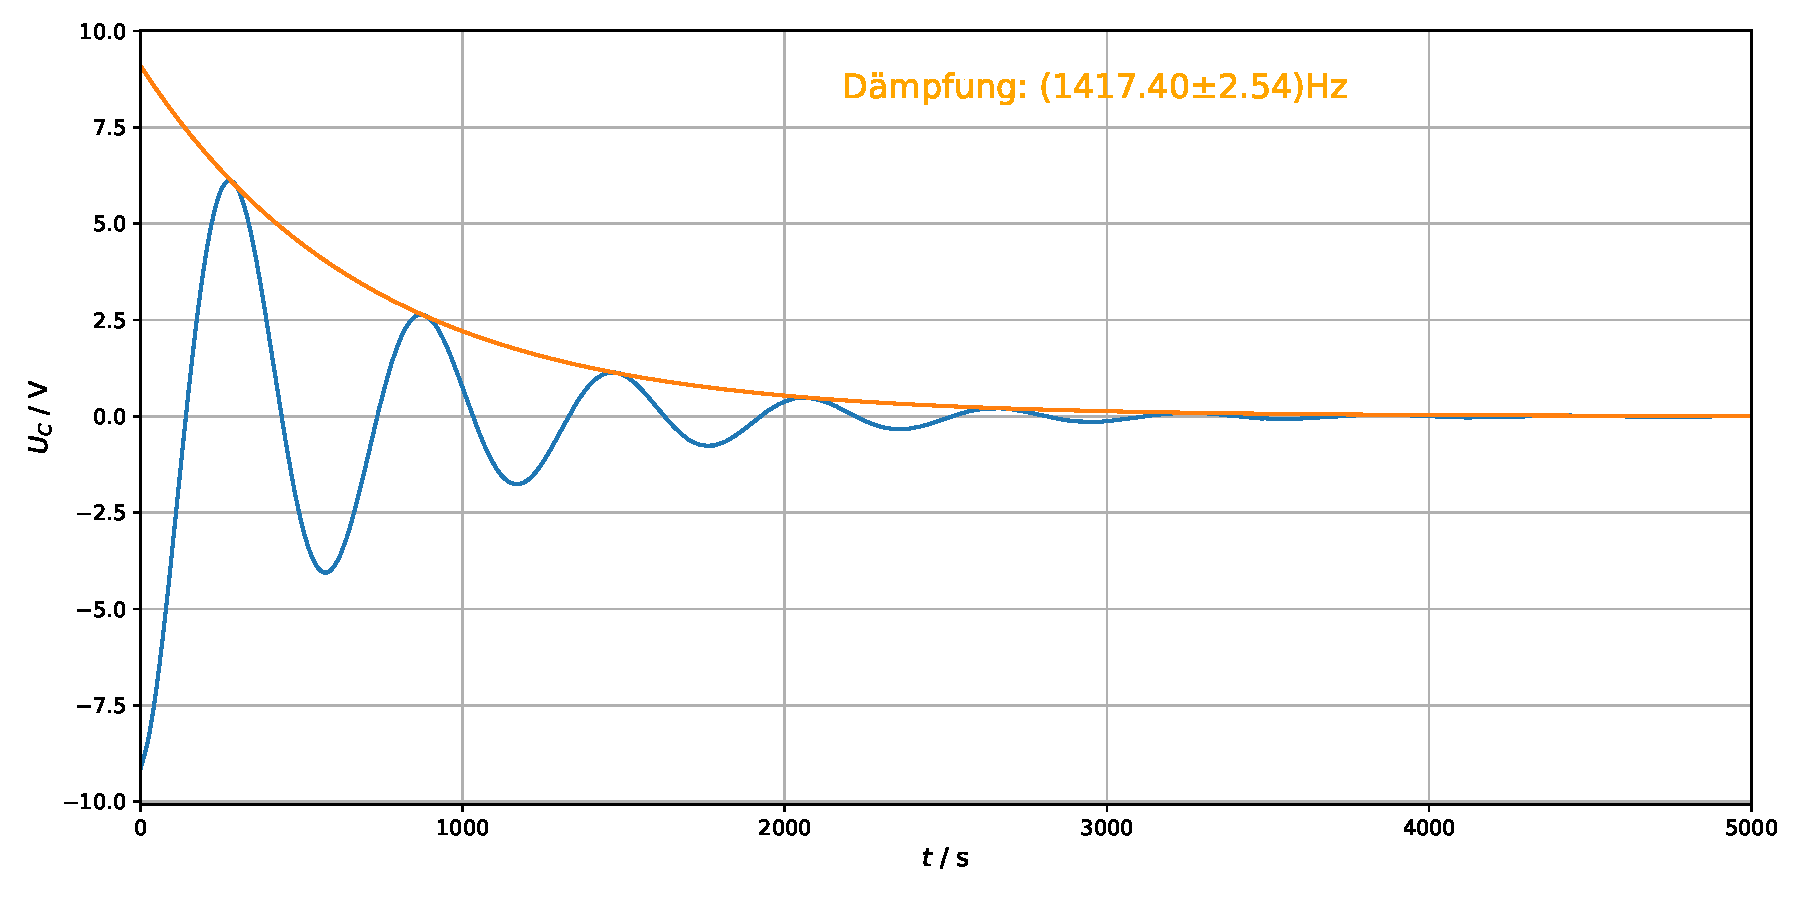
\includegraphics[width=\textwidth]{plots/einhuellend/exp_einhuellend4_2.pdf}
\caption{Mittels Python berechnete exponentiell Einhüllende für die zweite Messung des $20\Omega$ Widerstands.}
\end{figure}
\begin{figure}[h]
\centering
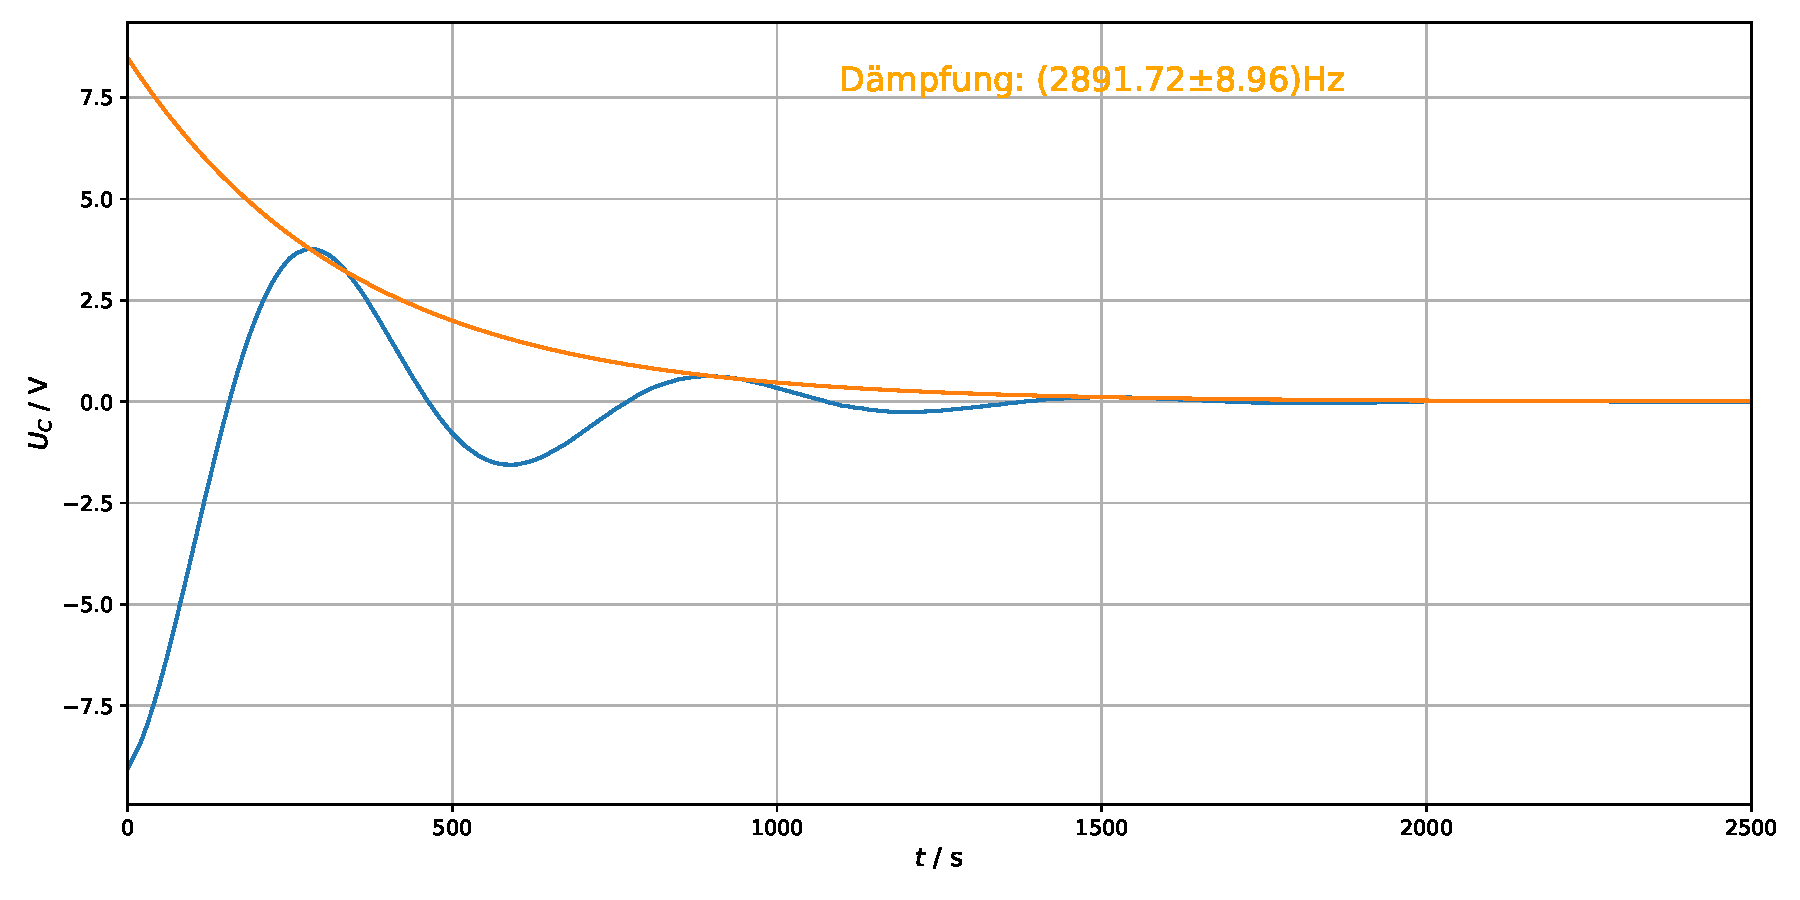
\includegraphics[width=\textwidth]{plots/einhuellend/exp_einhuellend5_2.pdf}
\caption{Mittels Python berechnete exponentiell Einhüllende für die zweite Messung des $47\Omega$ Widerstands.}
\end{figure}

\end{document}